% ------------------------------------------------------------------------
% ------------------------------------------------------------------------
% Modelo de trabalho acadêmico (Dissertações e Teses) do Programa de Pós-
% graduação em Física da Universidade Federal de Minas Gerais.
% Esse modelo é baseado na classe abntex2 (http://www.abntex.net.br)
% 
% ------------------------------------------------------------------------
% ------------------------------------------------------------------------

\documentclass[
    % -- opções da classe memoir --
    12pt,       % tamanho da fonte
    openright,  % capítulos começam em pág ímpar (insere página vazia caso preciso)
    twoside,    % para impressão em frente e verso. Oposto a oneside ---- Este comando ajusta automaticamente as margens
    a4paper,    % tamanho do papel. 
%   brazil,     % idioma adicional para hifenização
    english     % o último idioma é o principal do documento
    ]{abntex2}

% ---
% Pacotes básicos
% ---
\usepackage{lmodern}            % Usa a fonte Latin Modern
\usepackage[T1]{fontenc}        % Selecao de codigos de fonte.
\usepackage[utf8]{inputenc}     % Codificacao do documento (conversão automática dos acentos)
\usepackage{indentfirst}        % Indenta o primeiro parágrafo de cada seção.
\usepackage{color}              % Controle das cores
\usepackage{graphicx}           % Inclusão de gráficos
\usepackage{microtype}          % para melhorias de justificação
\usepackage{relsize}            % usado para definir tamanho de fontes no sumário
% ---

% ---
% Pacotes úteis 
% ---
\usepackage[final]{pdfpages}        % Para incluir arquivos pdf externos
\usepackage{amsmath,amssymb,amsthm,mathtools} % Pacote para melhorar apresentação de fórmulas matemáticas, símbolos e teoremas, respectivamente
\usepackage{bm}                     % Símbolos matemáticos em negrito
\usepackage{pdflscape}              % Pacote para adicionar páginas em formato paisagem
\usepackage{multirow}               % Permite criar céluas com várias colunas ou linhas em tabelas
\usepackage{adjustbox}              % Pacote para ajustar a largura e altura de objetos como tabelas
\usepackage[makeroom]{cancel}
%\usepackage{imakeidx}              % Gera o índice

% ---
\usepackage{chngcntr}
\counterwithout{equation}{section} % undo numbering system provided by phstyle.cls
\counterwithin{equation}{chapter}  % implement desired numbering system
% ---

\usepackage{lipsum}  % pacote usado para gerar os textos dos apêndices e anexos

% ---
% Pacotes de citações
% ---
%\usepackage[brazilian,hyperpageref]{backref}  % Inclui um link nas referências para a página onde o documento foi citado.
\usepackage[hyperpageref]{backref}
\usepackage{cite}
\usepackage[fixlanguage]{babelbib}
%\selectbiblanguage{english}


% --- 
% CONFIGURAÇÕES DE PACOTES
% --- 

% ---
% Configurações do pacote backref
% Usado sem a opção hyperpageref de backref
\renewcommand{\backrefpagesname}{Cited on page(s):~}
% Texto padrão antes do número das páginas
\renewcommand{\backref}{}
% Define os textos da citação
\renewcommand*{\backrefalt}[4]{
    \ifcase #1 %
        No citation in text.%
    \or
        Cited in page #2.%
    \else
    Cited #1 time(s) in pages #2.%
    \fi}%
% ---

% ---
% Informações de dados para CAPA e FOLHA DE ROSTO
% ---
\titulo{Synchronization of Phase Oscilators}
\autor{Kevin Liu Rodrigues}
\local{Belo Horizonte}
\data{2020}
\orientador{Ronald Dickman}
\coorientador{Kevin Wood}
\tipotrabalho{Tese (Doutorado)}
\preambulo{Tese apresentada ao Programa de Pós-Graduação em Física do Instituto de Ciências Exatas da Universidade Federal de Minas
Gerais como requisito parcial para obtenção do título de Doutor em Ciências.}


% ---
% Configurações de aparência do PDF final
% ---
% alterando o aspecto da cor azul
\definecolor{blue}{RGB}{41,5,195}

% informações do PDF
\makeatletter
\hypersetup{
    %pagebackref=true,
    pdftitle={Synchronization of Phase Oscillators}, 
    pdfauthor={Kevin Liu Rodrigues},
    pdfsubject={\imprimirpreambulo},
    pdfcreator={LaTeX with abnTeX2},
    pdfkeywords={oscilador}{oscillator}{fisica}{physics}{tese}{thesis}{abnt}{latex}{abntex}{abntex2}{trabalho acadêmico}, 
    colorlinks=true,                   % false: boxed links; true: colored links
    linkcolor=blue,                    % color of internal links
    citecolor=blue,                    % color of links to bibliography
    filecolor=magenta,                 % color of file links
    urlcolor=blue,
    bookmarksdepth=4
}
\makeatother
% --- 

% --- 
% Espaçamentos entre linhas e parágrafos 
% --- 

% O tamanho do parágrafo é dado por:
\setlength{\parindent}{1.3cm}

% Controle do espaçamento entre um parágrafo e outro:
\setlength{\parskip}{0.2cm}  % tente também \onelineskip

% ---
% compila o indice, caso haja.
% ---
%\makeindex
% ---

% ---
% Comandos
% ---
\newcommand{\myint}{\int}                 % integral style
\newcommand{\ddt}[1]{\dot{#1}}            % time derivative style
\newcommand{\phase}{\theta}               % oscillator phase notation
\newcommand{\phaserot}{\varphi}           % oscillator phase notation in rotating frame
\newcommand{\nfreq}{\omega}               % oscillator natural frequency notation
\renewcommand{\vec}[1]{\bm{#1}}           % vector style
\newcommand{\kc}{K}                       % Kuramoto coupling notation
\newcommand*{\chirdef}{N\left[ \left< \left< |v| \right>_t^2 \right>_s - \left< \left< |v| \right>_t \right>_s^2 \right]}
\newcommand*{\chipsidef}{N\left[ \left< \left< |\psi| \right>_t^2 \right>_s - \left< \left< |\psi| \right>_t \right>_s^2 \right]}
\DeclarePairedDelimiter\ceil{\lceil}{\rceil}
\DeclarePairedDelimiter\floor{\lfloor}{\rfloor}

% ----
% Início do documento
% ----
\begin{document}

% Seleciona o idioma do documento (conforme pacotes do babel)
\selectlanguage{english}
%\selectlanguage{brazil}

% Retira espaço extra obsoleto entre as frases.
\frenchspacing 

% ----------------------------------------------------------
% ELEMENTOS PRÉ-TEXTUAIS
% ----------------------------------------------------------
\pretextual


% ---
% Folha de rosto
% (o * indica que haverá a ficha bibliográfica e deverá ser usado para teses 
%   e dissertações. Para projetos, favor retirar o *)
% ---
\imprimirfolhaderosto*
% ---

% ---
% Inserir a ficha bibliografica
% ---

%  A ficha catalografica, preparada pela biblioteca do departamento de física da UFMG é
% um elemento obrigatório para teses e dissertações. Inclua o arquivo pdf fornecido de acordo
% com o comando abaixo, modificando o nome e a localização do arquivo quando necessário.
%
\begin{fichacatalografica}
    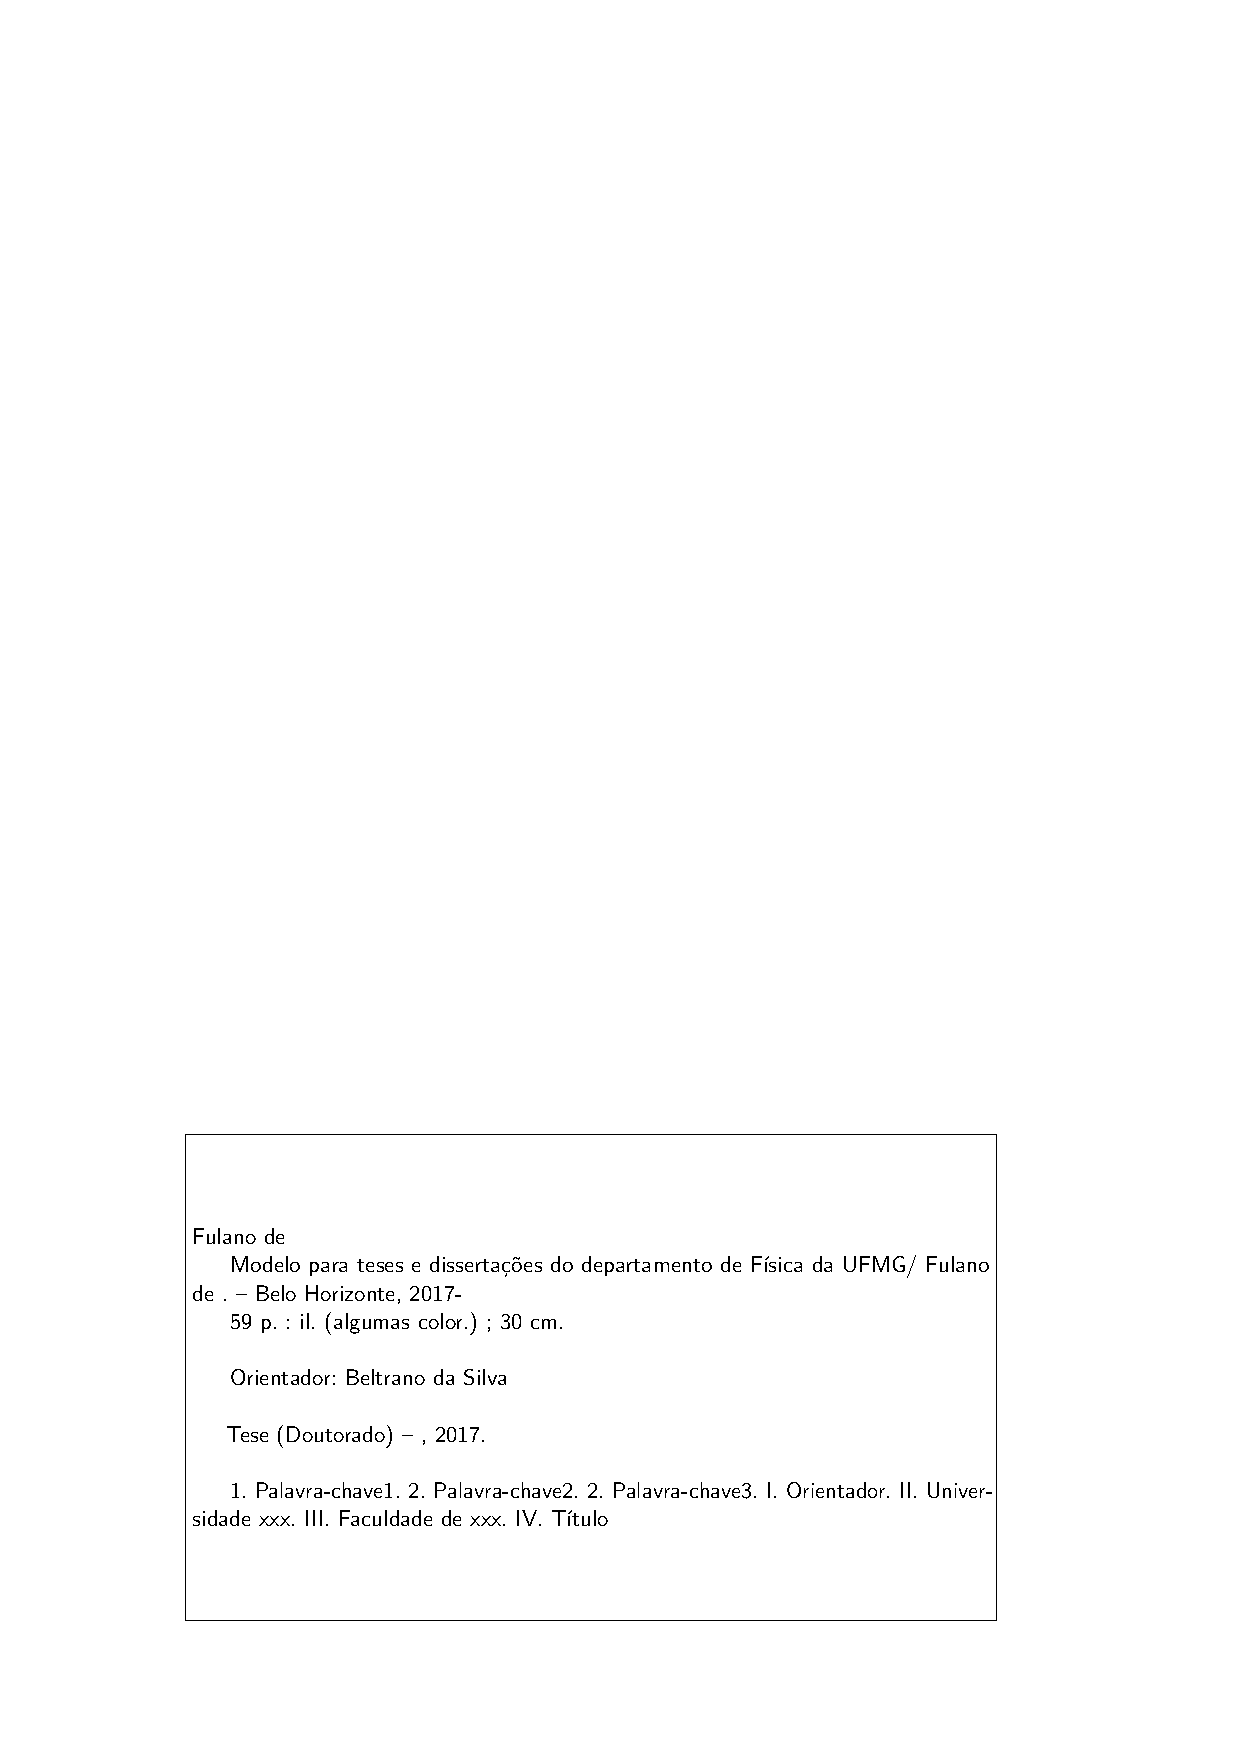
\includepdf{fig/ficha-catalografica.pdf}
\end{fichacatalografica}

% ---
% Inserir folha de aprovação
% ---

% A folha de aprovação é um elemento obrigatório da versão final do trabalho e deverá ser incluído
% conforme comando abaixo.
%
% TODO: na versao final incluir a ficha de aprovacao
\begin{folhadeaprovacao}
     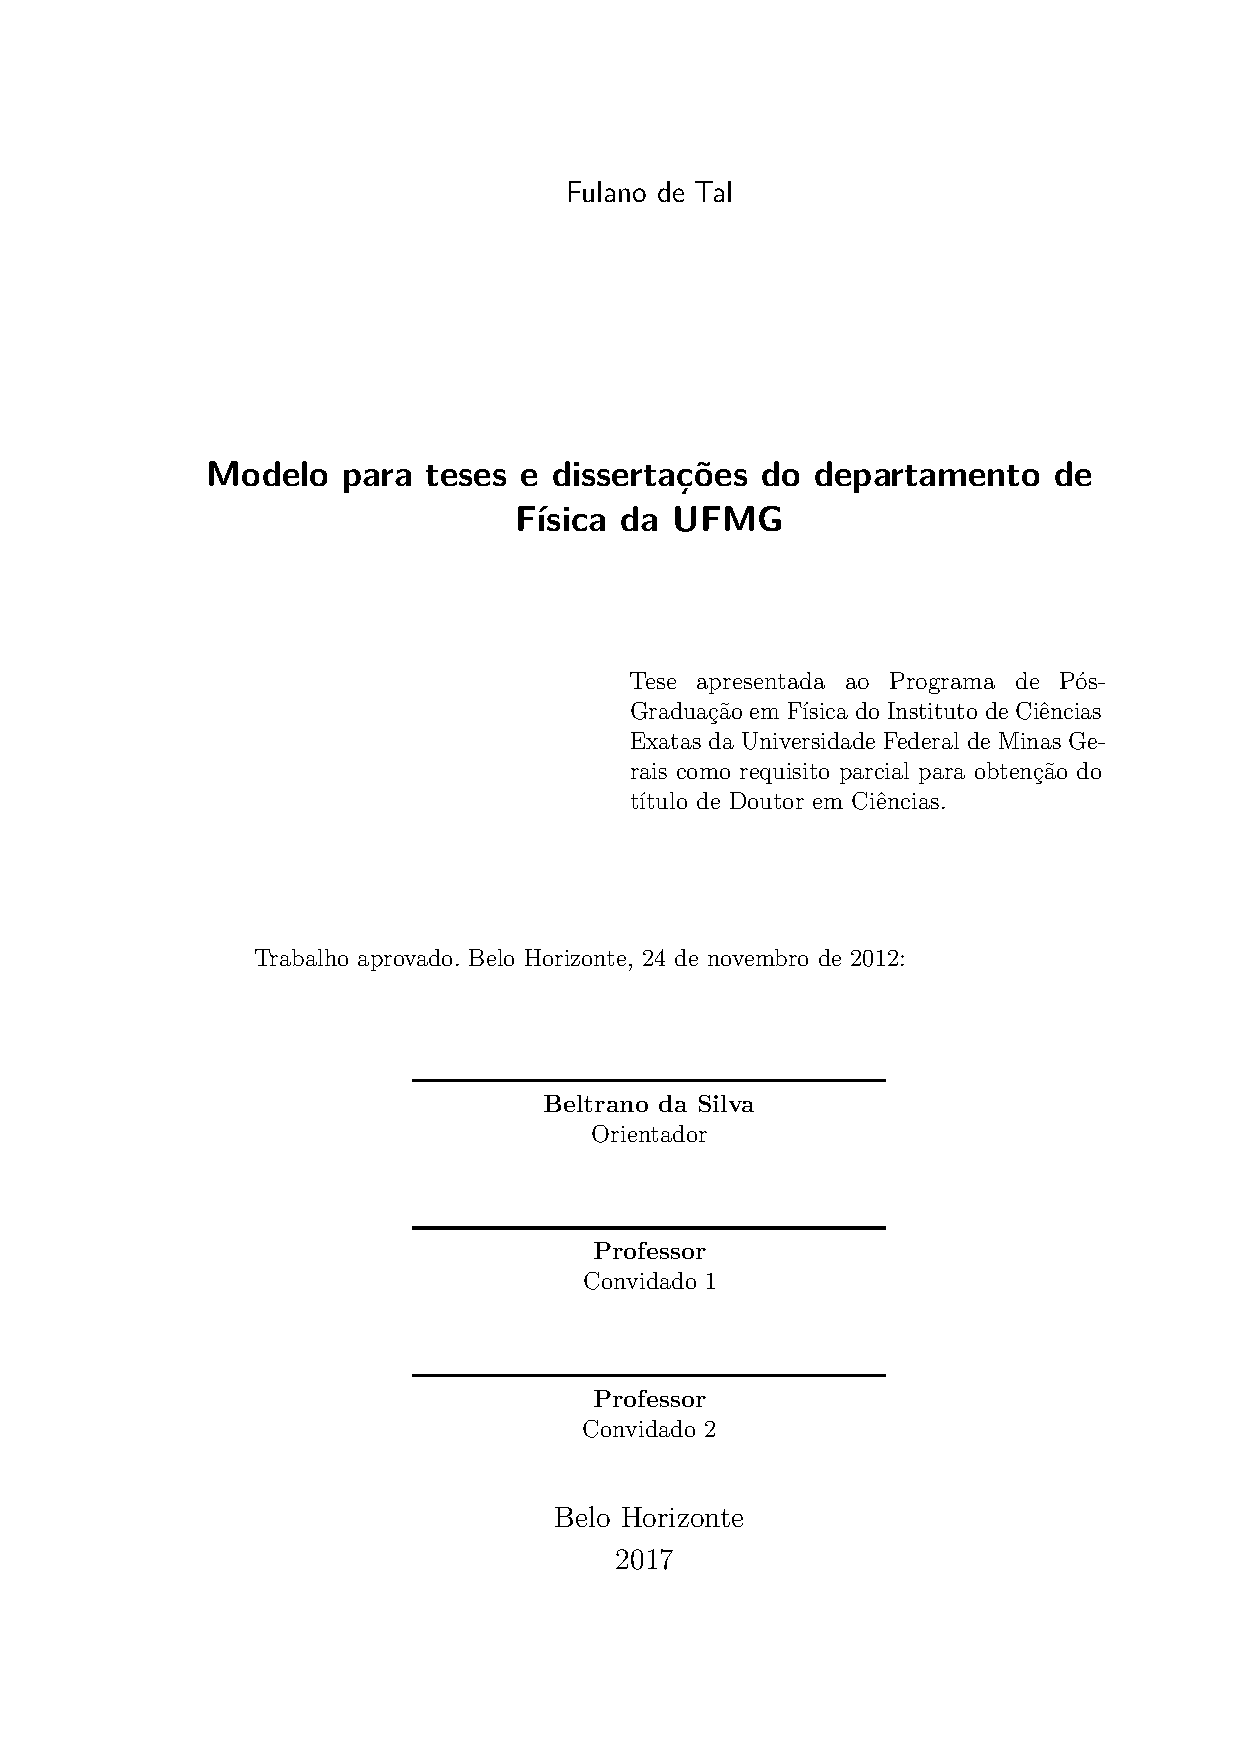
\includepdf{fig/folhadeaprovacao.pdf}
\end{folhadeaprovacao}
%


% ---
% Dedicatória - OPCIONAL
% ---
%\begin{dedicatoria}
%   \vspace*{\fill}
%   \centering
%   \noindent
%   \textit{\textbf{Dedicatória. Elemento opcional. Não há formatação a ser seguida.}\\
%    Este trabalho é dedicado às crianças adultas que,\\
%   quando pequenas, sonharam em se tornar cientistas.} \vspace*{\fill}
%\end{dedicatoria}
% ---

% ---
% Agradecimentos
% ---
\begin{agradecimentos}
Os agradecimentos são obrigatórios para os bolsistas e opcional para os demais. 
\end{agradecimentos}
% ---

% ---
% Epígrafe - OPCIONAL
% ---
%\begin{epigrafe}
%    \vspace*{\fill}
%	\begin{flushright}
%		\textit{\textbf{Epígrafe. Elemento opcional. Não há formatação a ser seguida.}\\
%		``Não vos amoldeis às estruturas deste mundo, \\
%		mas transformai-vos pela renovação da mente, \\
%		a fim de distinguir qual é a vontade de Deus: \\
%		o que é bom, o que Lhe é agradável, o que é perfeito.\\
%		(Bíblia Sagrada, Romanos 12, 2)}
%	\end{flushright}
%\end{epigrafe}
% ---

% ---
% RESUMOS
% ---

% resumo em português
\setlength{\absparsep}{18pt} % ajusta o espaçamento dos parágrafos do resumo
\begin{resumo}
\begin{otherlanguage*}{brazil}
O Resumo em português é um elemento obrigatório. Consiste de uma síntese de pontos relevantes com apresentação do objetivo, métodos,
técnicas, resultados e conclusões. Deve apresentar, abaixo, as palavras-chave relacionadas ao trabalho. Não pode exceder uma página.

\vspace{\onelineskip}
 
\noindent 
 \textbf{Palavras-chave}: Modelo, Tese, Dissertação, Projeto
\end{otherlanguage*}{brazil}

\end{resumo}

% resumo em inglês
\begin{resumo}[Abstract]
%\begin{otherlanguage*}{english}
The abstract and keywords, in English, are also mandatory and must fit in one page.
\vspace{\onelineskip}
 
\noindent 
\textbf{Keywords}: Template, Dissertations, Thesis, Projects.
%\end{otherlanguage*}

\end{resumo}

% ---
% LISTAS - CONTEÚDO DE CARÁTER OPCIONAL
% ---
% ---
% AS LISTAS DE ILUSTRAÇÕES, TABELAS, ABREVIATURAS E SIGLAS E SÍMBOLOS SÃO ELEMENTOS OPCIONAIS.
% RESSALTA-SE A IMPORTÂNCIA DE SE AO UTILIZAR TAIS LISTAS INCLUIR CORRETAMENTE NO LATEX UM TÍTULO
% PARA CADA FIGURA OU TABELA AO INVÉS DE DEIXAR A LEGENDA COMPLETA, QUE É, EM GERAL, MUITO GRANDE
% E POUCO INSTRUTIVA. ISTO É FEITO COM O SEGUINTE COMANDO: \caption[título da figura]{Legenda da figura}
% ---

% ---
% inserir lista de ilustrações - OPCIONAL
% ---
%\pdfbookmark[0]{\listfigurename}{lof}
%\listoffigures*
%\cleardoublepage
% ---

% ---
% inserir lista de tabelas - OPCIONAL
% ---
%\pdfbookmark[0]{\listtablename}{lot}
%\listoftables*
%\cleardoublepage
% ---

% ---
% inserir lista de abreviaturas e siglas - OPCIONAL
% ---
%\begin{siglas}
%  \item[ABNT] Associação Brasileira de Normas Técnicas
%  \item[abnTeX] ABsurdas Normas para TeX
%\end{siglas}
% ---

% ---
% inserir lista de símbolos - OPCIONAL
% ---
%\begin{simbolos}
%  \item[$ \Gamma $] Letra grega Gama
%  \item[$ \Lambda $] Lambda
%  \item[$ \zeta $] Letra grega minúscula zeta
%  \item[$ \in $] Pertence
%\end{simbolos}
% ---



% ---
% O SUMARIO É OBRIGATÓRIO
% ---

% ---
% inserir o sumario
% ---
\pdfbookmark[0]{\contentsname}{toc}
\tableofcontents*
\cleardoublepage
% ---




% ----------------------------------------------------------
% ELEMENTOS TEXTUAIS
% ----------------------------------------------------------
\textual

\chapter*{Introduction}

In 1951 the Belousov-Zhabotinsky class of chemical reactions were created for the first time in a laboratory. This feat marked an
upheaval in thermodynamics, which had now been shown, experimentally, to be ruled by non-equilibrium dynamics even for long mixing
times. This generated for the first time interest in the field of coupled oscillators by the broader scientific community. In the
decades that followed, other areas of research independently led to the same interests. In 1958, Norbet Weiner at MIT was looking at
power spectra from brain scans and decided that there must be some kind of synchronization amongst coupled, periodically-firing,
neurons. Also inspired by many biological rhythms observed in nature, Arthur Winfree published in 1967 a paper on the mathematical
modelling of interacting oscillators. Winfree defined a phase oscillator as an abstraction of any system that possesses periodicity. As
such, a complicated periodic process inside a living cell could be described by a single real number, between $0$ and $2\pi$, and its
rate of change. The major simplification comes from the fact that when two such phase oscillators interact, each influences
\textit{only} the rate of change in phase of the other. Their trajectories in phase space are assumed to remain closed loops, and thus
the only effective change can be modeled as a change in the speed at which they traverse it.

Seven years after Winfree's 1967 paper, the young Japanese scientist Yoshiki Kuramoto recognized what made Winfree's model hard to
solve. He proposed a modified version of it, assuming a particular form for the coupling between oscillators. This led to an arguably
less realistic model, but one which Kuramoto was cunningly able to solve. This modified version, together with its solution, would
later be recognized as the Kuramoto model, becoming one of the major founding stones in the field.

Since then, a plethora of novel coupled oscillator models have been put forward. One class deals with discrete phase oscillators, in
which the phase that describes a unit is related to a finite set of possible values. Discrete-phase models are used to describe systems
which exhibit markedly distinct states. An example of such a system is interacting neurons, where one can identify the three distinct
phases of a neuron as firing, refractory and ready-to-fire.

Another element present in some models is stochasticity in the dynamics, which is deterministic in the Kuramoto model. The element of
stochasticity may be included to account for noise, such as in models of open systems that interact with a heat bath.

Here we consider discrete-phase models with three possible phase states, and stochasticity plays a role in the rate of change of the
phase state of each unit, being the probability of ``jumping'' to the next state per unit time. This model was introduced by Kevin
Wood, C.  Van den Broeck, R. Kawai and Katja Lindenberg \cite{Wood06a}, with the main motivation of finding the simplest possible
dynamics between phase oscillators that still led to a phase transition to synchrony. Initial investigations focused mainly on square
lattices and all-to-all connections, exposing the ubiquity of this type of self-organization. Often times, networks of coupled
oscillators observed in nature possess neither of these two. Neurons, fireflies and cardiac cells are all examples of systems that do
not operate on lattices or complete-graph networks. One common type of interaction network observed in real systems is a mix between
local and global interactions. Various algorithms have been proposed for the generation of such intermediate connectivity graphs, some
of which generate small-world networks, characterized by the presence of long-range interactions while preserving strong local
clustering.

A particular example for the generation of small-world networks is the Watts-Strogatz algorithm, which randomly breaks connections on
an existing graph and re-creates them between random vertices. When applied to certain starting graphs with strong local clustering,
the result is a small-world network. Here we investigate how the dynamics of the three-phase oscillator model unfolds on such networks,
via simulation and a mean-field analysis.

\chapter{Kuramoto Model}
\label{chap:kuramoto}


In this chapter we describe the Kuramoto model, its dynamics and self-consistency arguments that allow for a synchronous phase to
emerge at some critical coupling. To do this, an order parameter is introduced together with a mean-field (MF) approximation. The
stability analysis of the solutions of the Kuramoto model took decades to develop and led to some very anti intuitive findings, such as
the fact that the disordered phase for weak coupling is not stable, but neutrally stable, and is related to Landau damping in plasma
physics.  Nonetheless, the two branches of solutions identified in Kuramoto's initial work don't require solving the original set of
equations, but rather rely on assuming macroscopic behaviors for the system and tracing back what implications they have for the
microscopic dynamics.  This feedback from macro to micro is central to Kuramoto's self-consistency arguments, which helped popularize
his model by lowering the barrier of entry to understanding synchronization in complex systems. Much of the discussion developed in
this section are reproductions from the notes of da Fonseca Abud\cite{da_Fonseca_2018}.


\section{Definition}

The Kuramoto model consists of a collection of phase oscillators (``units'') which are all coupled to each other. We start with a
collection of $N$ oscillators and then take the continuous limit with $N \to \infty$. Each unit $j$ at time $t$ is described by its
phase value $\phase_j(t)$ and its natural frequency $\nfreq_j$, which is its rate of change in phase in isolation, and is assumed to be
constant. The natural frequencies $\vec{\nfreq}\equiv \{\nfreq_1,\dots,\nfreq_N\}$ are assumed to follow some frequency distribution
$\vec{\nfreq} \sim g(\vec{\nfreq})$ which is symmetric about some frequency $\bar{\nfreq}$, and unimodal. While the rate of change of
an isolated unit is time independent, the coupling between oscillators makes $\ddt{\phase_j}$ a function of the entire phase
configuration $\vec{\phase}(t) \equiv \{ \phase_1(t), \dots, \phase_N(t)\}$.

The biologically inspired Winfree model states that, at every instant, each oscillator sends a signal of strength $P(\phase)$ and
responds by adjusting its own phase value proportionally to $Q(\phase)$ when receiving signals from other units, which is captured in
the equation:

\begin{equation}
    \ddt{\phase_j} = \nfreq_j + \frac{1}{N}\sum^{N}_{k}P(\phase_k)Q(\phase_j), \qquad j=1,...,N
    \label{winfreeeq}
\end{equation}

In the special case where the product $P(\phase_k)Q(\phase_j)$ depends only on the phase difference between oscillators $j$ and $k$,
the product inside the summation can be written as a single function called the kernel $F$: $P(\Delta \phase)Q(\Delta \phase) \equiv
F(\Delta \phase)$. If furthermore the kernel is proportional to the sine function, then Winfree's equation~(\ref{winfreeeq}) becomes
the Kuramoto model:

\begin{equation}
    \ddt{\phase_j} = \nfreq_j + \frac{\kc}{N}\sum^{N}_{k}\sin(\phase_k - \phase_j), \qquad j=1,...,N
    \label{kura}
\end{equation}

\noindent where $\kc \geq 0$ is a real constant which describes the coupling strength between any pair of oscillators.

\section{Mean-field and order parameter}

To determine if the microscopic collection of phases represents a synchronized macro state, we introduce the Kuramoto order parameter
$R$. It maps a phase configuration $\vec{\phase}$ to a magnitude by representing the phase values as complex numbers on the unit circle
and performing a complex summation:

\begin{align}
    R(\vec{\phase})e^{i\phi(\vec{\phase})} &\equiv \frac{1}{N} \sum^{N}_{k} e^{i\phase_k(t)}
    \label{kuramotoop}
\end{align}

\noindent where $i=\sqrt{-1}$ and $\phi(\vec{\phase})\in[0,2\pi)$ is the resulting polar angle of the summation. Thus $R( \vec{\phase})
\in [0,1]$ determines the overall macroscopic alignment between phase values. With this definition the equations of motion can be
re-written as:

\begin{align}
    \ddt{\phase_j} &= \nfreq_j + \frac{\kc}{N}\sum^{N}_{k}\sin(\phase_k - \phase_j) \notag \\
                   &= \nfreq_j + \kc \operatorname{Im}\left( \frac{1}{N}\sum^{N}_{k} e^{i(\phase_k-\phase_j)} \right) \notag \\
                   &= \nfreq_j + \kc R(\vec{\phase}) \operatorname{Im}\left( e^{i(\phi(\vec{\phase}) - \phase_j)} \right) \notag \\[18pt]
    \ddt{\phase_j} &= \nfreq_j + \kc R(\vec{\phase}) \sin ( \phi(\vec{\phase}) - \phase_j )
    \label{kuramf}
\end{align}

We see that the equations of motion are now written in terms of the mean fields $R(\vec{\phase})$ and $\phi(\vec{\phase})$. In
particular, if the fields are constant ($\ddt{R} = \ddt{\phi}=0$) then the equations of motion become decoupled and can be solved.

The collective oscillations observed in real systems tell us that the macroscopic steady-state solution of stable synchronized
oscillations should indeed have constant $R>0$ while $\phi$ increases linearly with time (the system rotates synchronously with
constant phase speed).  Thus, $\phi=\Omega t$ and both $R$ and $\Omega$ are constant. Even though $\phi$ itself is not constant, it
turns out that the rotational symmetry of equation~(\ref{kuramf}) allows us to decouple the equations by moving to a rotating frame of
reference with the following substitution:

\begin{align}
    \forall j: \quad \phase_j(t) &= \phaserot_j(t) + \Omega t \notag\\
    &\Downarrow \notag\\
    \ddt{\phaserot_j} + \Omega &= \nfreq_j - \kc R \sin ( \phaserot_j ) \notag\\[10pt]
    \ddt{\phaserot_j} &= (\nfreq_j-\Omega) - \kc R \sin ( \phaserot_j )
    \label{kurarot}
\end{align}

Another macroscopic behavior observed in nature is the more trivial one, with no synchronization at all. In this state the phase
configuration is evenly distributed over all possible values, leading to constant $R=0$, and is also described by
equation~(\ref{kurarot}). Inspection of this equation shows that when $|\nfreq_j - \Omega| \leq \kc R$ there is some phase value for
which $\ddt{\phaserot_j}=0$, and thus oscillators become phase-locked when attaining this value. When $|\nfreq_j - \Omega| > \kc R$,
the $\phaserot_j$ can never stop varying and will permanently drift. For a synchronized solution we then expect two groups of
oscillators:

\begin{itemize}
    \item \textbf{Phase-Locked} $|\nfreq_j - \Omega|\leq \kc R$: A group of oscillators with natural frequencies close enough to
        $\Omega$ will become phase locked and sync.
    \item \textbf{Drifting} $|\nfreq_j - \Omega| > \kc R$: Remaining oscillators with frequencies too far from the generated mean-field
        will remain drifting ahead or behind the synced group.
\end{itemize}

Since we postulate that $R$ is time independent, self-consistency requires that the phase distribution generated by the drifting
oscillators must be stationary, otherwise $R$ would not be constant.

\section{Continuous Limit}

In the continuous limit $N\to \infty$, the distribution of oscillator phases can be written as the joint probability density in phases
$\phaserot$ and natural frequencies $\nfreq$ as:

\begin{equation*}
	P(\phaserot_j, \nfreq_j,t) \to p(\phaserot, \nfreq,t) \qquad \phaserot \in [-\pi, \pi) \qquad \nfreq \in (-\infty, \infty)
\end{equation*}

\noindent For given values of $\phaserot$ and $\nfreq$, the evolution follows

\begin{equation}
	\ddt{\phaserot} = (\nfreq - \Omega) - \kc R \sin(\phaserot).
	\label{eqmotioncontinuous}
\end{equation}

\noindent The density of oscillators with phase $\phaserot$ is then given by the marginal distribution:

\begin{align*}
    n(\phaserot) = \myint_{-\infty}^{\infty} p(\phaserot, \nfreq,t) d\nfreq
\end{align*}

\noindent which by the definition of conditional probability gives:

\begin{align*}
    n(\phaserot) = \myint_{-\infty}^{\infty} p(\phaserot | \nfreq)g(\nfreq) d\nfreq
\end{align*}

\noindent where $p(\phaserot|\nfreq)$ is the conditional probability density that an oscillator with given natural frequency
$\nfreq$ has phase value $\phaserot \equiv \phaserot(t)$ at time $t$.

By using the subscripts $L$ and $D$ to indicate the \textit{phase-locked} and \textit{drifting} groups, we get the expression for the
total density:

\begin{gather}
    n(\phaserot) = n_L(\phaserot) + n_D(\phaserot) \notag\\[10pt]
    n(\phaserot) = \myint_{|\nfreq - \Omega|\leq \kc R} p_L(\phaserot|\nfreq,t) g(\nfreq) d\nfreq + \myint_{|\nfreq - \Omega| > \kc R} p_D(\phaserot|\nfreq,t) g(\nfreq) d\nfreq
    \label{density}
\end{gather}

The conditional probability for the phase-locked group can then be obtained by solving the equation of motion~(\ref{kurarot}), and for
the drifting group it can be derived by the self-consistency assumption that it must be a stationary distribution in order to have a
time-independent order parameter.

\section{Phase distribution of phase-locked oscillators}

For the phase locked group we know that for $t \to \infty$, $\ddt{\phaserot}=0$ for some value of $\phaserot^\star$ and $\nfreq$. Thus,
we solve equation~(\ref{eqmotioncontinuous}) to obtain:

\begin{gather}
    \phaserot^\star = \arcsin \left( \frac{\nfreq - \Omega}{\kc R} \right), \quad
    \phaserot^\star \in \left[ -\frac{\pi}{2}, \frac{\pi}{2} \right] \notag
\end{gather}

Therefore, the conditional distribution of $\phaserot$ given $\nfreq$ is a Dirac delta function centered around $\phaserot^\star$,
since this is an attractor for all oscillators with natural frequency $\nfreq$.

\begin{gather}
    \label{lockedprob}
    p_L(\phaserot | \nfreq) = \delta\left[ \phaserot - \arcsin \left( \frac{\nfreq - \Omega}{\kc R} \right) \right], \quad
    \phaserot \in \left[ -\frac{\pi}{2}, \frac{\pi}{2} \right]
\end{gather}

We now perform the left integral in equation~(\ref{density}) to find the density of phase locked oscillators to obtain:
\begin{align*}
    n_L(\phaserot) &= \myint_{\Omega - \kc R}^{\Omega + \kc R} \delta\left[ \phaserot - \phaserot^\star \right] g(\nfreq) d\nfreq
\end{align*}

\noindent but $\nfreq = \Omega + \kc R \sin\phaserot^\star$ and $d\nfreq = \kc R \cos \phaserot^\star d\phaserot^\star$ and thus

\begin{align}
    n_L(\phaserot) &= \myint_{-\frac{\pi}{2}}^{\frac{\pi}{2}} \delta \left[ \phaserot - \phaserot^\star \right] g(\Omega + \kc R \sin
    \phaserot^\star) \kc R \cos \phaserot^\star d\phaserot^\star \notag\\[10pt]
    n_L(\phaserot) &=
    \begin{cases}
        g(\Omega + \kc R \sin\phaserot) \kc R \cos\phaserot \quad &|\phaserot| \leq \frac{\pi}{2}\\
        0 & |\phaserot| > \frac{\pi}{2}
    \end{cases}
    \label{densitylocked}
\end{align}

Equation~(\ref{densitylocked}) shows us that the phase locked oscillators are distributed in the half-moon around the order parameter,
in accord with direct simulations of the equations of motion. Since the $\phaserot$ values are phase-locked, the probability
distribution of synchronized oscillators $n_L$ is also time independent, in addition to $n$.

\section{Phase distribution of drifting oscillators}

In order to derive the distribution of phases for drifting oscillators, for which $|\nfreq - \Omega| > \kc R$, consider an interval
$[\phaserot, \phaserot + \delta \phaserot ]$ in phase values. The fraction of oscillators with natural frequency $\nfreq \in [\nfreq',
\nfreq' + \delta\nfreq]$ inside this interval is given by:

\begin{align}
	\left[ \myint_{\phaserot}^{\phaserot + \delta \phaserot} p(\phaserot' | \nfreq) d\phaserot' \right] \delta \nfreq
	\label{count}
\end{align}

The change per unit time in the fraction of oscillators inside this interval is then given by the time derivative of~(\ref{count}), but
since all intervals endpoints $\nfreq$, $\delta\nfreq$ and $\phaserot$, $\delta\phaserot$ are fixed we have:

\begin{equation}
	\partial_t \left[ \myint_{\phaserot}^{\phaserot + \delta \phaserot} p(\phaserot' | \nfreq) d\phaserot' \right] =
	\myint_{\phaserot}^{\phaserot + \delta \phaserot}\partial_t p(\phaserot' | \nfreq) d\phaserot'
\end{equation}

\noindent Conservation of probability inside the interval $[\phaserot,\phaserot+\delta\phaserot]$ mandates that the net change in
probability must equal the difference between fluxes at the endpoints. The probability current is written as $j(\phaserot, \nfreq, t) =
p(\phaserot|\nfreq)\ddt{\phaserot}$

\begin{align}
	\myint_{\phaserot}^{\phaserot + \delta \phaserot}\partial_t p(\phaserot' | \nfreq) d\phaserot' = 
	\label{control_interval}
\end{align}

Intuitively, equation~(\ref{control_interval}) implies that the rate of change of probability inside the control interval is equal to
the difference of fluxes at the extremities of the interval. Dividing this expression by $\delta\phaserot$ and taking the limit of
$\delta\phaserot \to 0^+$ leads us to the continuity equation for the conservation of probability density of oscillators with natural
frequency $\nfreq$:

\begin{gather}
    \lim_{\delta\phaserot \to 0^+} \frac{p(\phaserot+\delta\phaserot | \nfreq)\ddt{\phaserot}(\phaserot+\delta\phaserot) - p(\phaserot | \nfreq)\ddt{\phaserot}(\phaserot)}{\delta\phaserot} = \partial_\phaserot \left[ p(\phaserot | \nfreq) \ddt{\phaserot}(\phaserot) \right]  \notag\\
    \lim_{\delta\phaserot \to 0^+} \partial_t \left[ \frac{1}{\delta\phaserot}\myint_{\phaserot}^{\phaserot + \delta \phaserot} p(\phaserot' | \nfreq) d\phaserot' \right] = \partial_t \left[ p(\phaserot | \nfreq) \right] \notag\\[10pt]
    \partial_t \left[ p(\phaserot | \nfreq) \right] - \partial_\phaserot \left[ p(\phaserot | \nfreq) \ddt{\phaserot}(\phaserot) \right] = 0
    \label{continuity}
\end{gather}

We have seen that requiring that the total phase distribution $n(\phaserot)$ be stationary implies that the distribution of
phase-locked oscillators $n_L(\phaserot)$ is also stationary. But since the distribution of drifting oscillators is given by
$n_D(\phaserot) = n(\phaserot) - n_L(\phaserot)$, it must also be stationary. Thus we have

\begin{gather}
    \partial_t [ n_D(\phaserot) ] = 0\notag\\
    \myint_{|\nfreq - \Omega| > \kc R} \partial_t [ p_D(\phaserot | \nfreq)] g(\nfreq) d\nfreq = 0
    \label{stationary_drift}
\end{gather}

Even though there are time-dependent forms for $p_D(\phaserot | \nfreq)$ that could satisfy equation~(\ref{stationary_drift}), the
assumption that it is indeed stationary ties up with the original assumption about the total density $n$ and the self consistency
argument, a central point in Kuramoto's original analysis. The condition $\partial_t [p_D(\phaserot | \nfreq)]=0$ for all $\phaserot$
thus imply, through the continuity equation~(\ref{continuity}), that $\partial_\phaserot [p_D(\phaserot |
\nfreq)\ddt{\phaserot}(\phaserot)]=0$ and so:

\begin{gather}
    p(\phaserot | \nfreq) \ddt{\phaserot}(\phaserot) = C(\nfreq) \notag\\
    \Downarrow \notag\\
    p_D(\phaserot | \nfreq) = \frac{C(\nfreq)}{(\nfreq - \Omega) - \kc R \sin \phaserot}
    \label{nD}
\end{gather}

In order to obtain the total density $n_D(\phaserot)$ we must marginalize the joint distribution $p_D(\nfreq | \nfreq)g(\nfreq)$. In
order to do that we need to find the value of $C$ as a function of $\nfreq$, $C(\nfreq)$. This can be done by using the normalization
condition $\int_{-\pi}^{\pi}p_D(\phaserot | \nfreq)d\phaserot=1$ which leads us to:

\begin{align}
    \frac{1}{C(\nfreq)} &= \myint_{-\pi}^{\pi}\frac{1}{\nfreq - \Omega - \kc R \sin \phaserot}d\phaserot
    \label{constantC}
\end{align}

\noindent Using equation~(2.551-3) from the integrals table~\cite{jeffrey2007table} with the condition $|\nfreq-\Omega| > \kc R$ we get
the solution:

\begin{align}
    a&=(\nfreq-\Omega) \qquad b=\kc R \notag\\[5pt]
    f(\phaserot) &= \arctan\frac{a\tan \frac{\phaserot}{2}+b}{\sqrt{a^2-b^2}} \notag\\[5pt]
    \myint\frac{1}{\pm a-b\sin \phaserot}d\phaserot &= \pm\frac{2}{\sqrt{a^2-b^2}}f(\phaserot) \qquad a^2 > b^2 \notag
\end{align}

\noindent which is positive for $\nfreq > \Omega + \kc R$ and negative for $\nfreq < \Omega - \kc R$. Substituting back into
equation~(\ref{constantC}) to obtain $C$ gives:

\begin{align}
    \frac{1}{C_\pm(\nfreq)} &= \pm\frac{2}{\sqrt{(\nfreq-\Omega)^2 - (\kc R)^2}} \left[ \lim_{\phaserot \to \pi^-} f(\phaserot) - \lim_{\phaserot \to (-\pi)^+} f(\phaserot) \right] \notag\\[10pt]
    C(\nfreq) &=
    \begin{cases}
        -\frac{\sqrt{(\nfreq-\Omega)^2 - (\kc R)^2}}{2\pi} \qquad &\nfreq < \Omega - \kc R \\[10pt]
        \frac{\sqrt{(\nfreq-\Omega)^2 - (\kc R)^2}}{2\pi} \qquad &\nfreq > \Omega + \kc R
    \end{cases}
    \label{constant}
\end{align}

Now, we use the expression for $C(\nfreq)$ to perform the integration in $\nfreq$ as defined in equation~(\ref{density}):

\begin{align}
    n_D(\phaserot) &= \myint_{-\infty}^{\Omega - \kc R} p_D(\phaserot | \nfreq)g(\nfreq)d\nfreq +
                      \myint_{\Omega + \kc R}^{\infty} p_D(\phaserot | \nfreq)g(\nfreq)d\nfreq \notag\\
                   &= \myint_{-\infty}^{\Omega - \kc R} \frac{C_-(\nfreq)}{(\nfreq - \Omega) - \kc R\sin\phaserot}g(\nfreq)d\nfreq +
                      \myint_{\Omega + \kc R}^{\infty} \frac{C_+(\nfreq)}{(\nfreq - \Omega) - \kc R\sin\phaserot}g(\nfreq)d\nfreq
                      \label{driftdensityintermediate}
\end{align}

To perform this integration we make use of the assumptions that $g$ is symmetric and unimodal. In addition, we also assume that the
frequency of global oscillations to which the system converges to, $\Omega$, is coincident with the point of symmetry of $g$. Namely,
we assume that $\Omega = \bar{\nfreq}$. With this assumption, $g(\Omega + x) = g(\Omega - x)$, allowing us to make the following change
of variables:

Substitute equation~(\ref{constant}) into (\ref{driftdensityintermediate}) and change variables $\nfreq -
\Omega = -x$ in the first integral and $\nfreq - \Omega = x$ in the second. Finally, we get the expression for the density of drifting
oscillators:

\begin{align}
    n_D(\phaserot) = \frac{1}{\pi}\myint_{\kc R}^\infty \frac{x\sqrt{x^2 - (\kc R)^2}}{x^2 - (\kc R\sin\phaserot)^2}g(x+\Omega)dx
    \label{densitydrift}
\end{align}


\section{Order Parameter}


In the rotating frame, the Kuramoto order parameter is given by the integral:

\begin{align}
    R = &\myint_{-\pi}^{\pi} e^{i\phaserot}n_L(\phaserot)d\phaserot + \myint_{-\pi}^{\pi} e^{i\phaserot}n_D(\phaserot)d\phaserot
\end{align}

From equation~(\ref{densitydrift}) we see that $n_D(\phaserot - \pi) = n_D(\phaserot)$, but $e^{i(\phaserot - \pi)} = -e^{i\phaserot}$,
and thus the rightmost integral is zero. The leftmost integral on the right hand side (RHS) can then be written with
equation~(\ref{densitylocked}) for the phase-locked oscillators.

\begin{align}
     R = &\kc R\myint_{-\pi/2}^{\pi/2} (\cos \phaserot + i \sin \phaserot ) \cos\phaserot g(\Omega + \kc R \sin\phaserot) d\phaserot
\end{align}

\noindent but since $g$ is symmetric around $\Omega$ we end up with

\begin{align}
     R = \kc R\myint_{-\pi/2}^{\pi/2} g(\Omega + \kc R \sin\phaserot) \cos^2\phaserot d\phaserot
     \label{finalkura}
\end{align}

Thus, we see that for a fixed value of the coupling strength $\kc$ there is always at least one solution for the order parameter $R$.
The trivial (disordered) solution is given by $R=0$. If $R$ is non-zero, then we can divide equation~(\ref{finalkura}) to obtain the
condition for the existence of the solution for that particular $\kc$:

\begin{align}
     \kc\myint_{-\pi/2}^{\pi/2} g(\Omega + \kc R \sin\phaserot) \cos^2\phaserot d\phaserot = 1
     \label{kc}
\end{align}

The simpler case of identical oscillators can be obtained from equation~(\ref{kc}) by setting $g(x) = \delta(x-\Omega)$ which results
in $\kc_c = 1$ as the critical coupling strength for such a network to attain synchronization.

For a general for of the natural frequency distribution $g$ we can obtain the critical coupling strength $\kc_c$ by expanding its
Taylor series around $\Omega$ and neglecting terms $\mathcal{O}(R)$ and higher. This is because when $\kc \to \kc_c^+$, then $R \to
0^+$ and so:

\begin{align}
    \frac{1}{\kc} &= \myint_{-\pi/2}^{\pi/2} \left[ g(\Omega) + g''(\Omega)\frac{(\kc R \sin\phaserot)^2}{2} + \mathcal{O}(R^3) \right] \cos^2\phaserot d\phaserot \\[10pt]
    \frac{1}{\kc_c} &= \lim_{R\to0^+} \myint_{-\pi/2}^{\pi/2} \left[ g(\Omega) + g''(\Omega)\frac{(\kc R \sin\phaserot)^2}{2} + \mathcal{O}(R^3) \right] \cos^2\phaserot d\phaserot
\end{align}

\noindent where $g'(\Omega)=0$ since $g(\Omega)$ is a maximum. Therefore the critical coupling is given by:

\begin{align}
    \kc_c = \frac{2}{\pi g(\Omega)}
\end{align}

As the coupling approaches the critical value from above, the order parameter scales as:

\begin{align}
    \frac{1}{\kc} &= \frac{1}{\kc_c} - \frac{\kc_c^2 R^2|g''(\Omega)| }{16} + \cancelto{0}{\mathcal{O}(R^3)} \notag\\
                  &\Downarrow \notag \\
    R(\kc) &= \frac{4}{\sqrt{\pi\kc_c^3|g''(\Omega)|}} \sqrt{\frac{\kc - \kc_c}{\kc_c}}
\end{align}

We see that the order parameter is sensitive to the curvature of $g$ at the maximum, growing ever more rapidly as $g$ becomes narrower.
In the limit of identical oscillators, and the order parameter becomes discontinuous at the transition.


\chapter{\label{chap:article} Stochastic discrete phase model}

In this chapter we define the discrete three state model for coupled oscillators. This is a reproduction
of~\cite{rodrigues2020synchronization}.

\section{Abstract}

A lattice of three-state stochastic phase-coupled oscillators exhibits a phase transition at a critical value of the coupling parameter
$a$, leading to stable global \textit{oscillations} (GO). On a complete graph, upon further increase in $a$, the model exhibits an
\textit{infinite-period} (IP) phase transition, at which collective oscillations cease and discrete rotational ($C_3$) symmetry is
broken. The IP phase does not exist on finite-dimensional lattices.  In the case of large negative values of the coupling no
synchronization is expected, but nonetheless it was shown that travelling-wave steady states are stable, displaying local order. Here,
we verify the IP phase in systems with long-range coupling but of lower connectivity than a complete graph and show that even for large
\textit{ positive} coupling, the system sometimes fails to reach global order. The ensuing travelling-wave state appears to be a
metastable configuration whose birth and decay (into the previously described phases) are associated with the initial conditions and
fluctuations.

\section{Introduction}

Systems of coupled oscillators exhibit diverse symmetry-breaking transitions to a globally synchronized state. In the paradigmatic
Kuramoto model, for instance, oscillators with distinct intrinsic frequencies $\omega_i$ coupled via their continuous phases $\theta_i$
can exhibit stable collective oscillations, breaking time-translation
invariance~\cite{Kuramoto84,Strogatz93,Strogatz00,StrogatzSync,Pikovsky01}.  Amongst discrete-phase models, the paper-scissors-stone
game is an example of a system with three absorbing states that can exhibit either global oscillations or spontaneous breaking of
discrete rotational ($C_3$) symmetry~\cite{Tainaka88,Tainaka89,Tainaka91,Itoh94,Tainaka94}. More recently, Wood and coworkers proposed
a family of models of phase-coupled three-state stochastic oscillators that undergo a phase transition to a state exhibiting global
oscillations (GO)~\cite{Wood06a,Wood06b,Wood07a,Wood07b} for sufficiently strong coupling.  We shall refer to these as Wood's cyclic
model~(WCM). Although the WCM also has $C_3$ symmetry, it has no absorbing state.  In addition to their intrinsic interest in the
context of non equilibrium phase transitions, this family of models serve as a highly simplified description of collective neuronal
behavior.


The first WCM~\cite{Wood06a} was found to undergo a second phase transition upon further increase of the coupling
\cite{assis2011infinite}, at which the period of oscillation becomes infinite, thereby breaking $C_3$ symmetry. In
\cite{assis2011infinite}, this infinite-period (IP) transition was studied on a complete graph (all-to-all coupling), and a novel order
parameter, involving the mean rate of change of the probability distribution, was proposed. On the basis of a nucleation scenario, the
authors of Ref. \cite{assis2011infinite} argued \textit{against} the existence of an IP transition on finite-dimensional lattices with
short-range interactions, but left open the question of its occurrence on networks with nonlocal interactions. Here we study a WCM on
(1) regular rings with interactions up to $2K$-neighbors, varying the interaction range $K$, and (2) small-world networks. Using
numerical simulations to study the order parameter and its variance, we verify the existence of GO and IP phase transitions on these
structures. For regular rings of $N$ nodes, the degree of connectivity is characterized by $\alpha \equiv K/N$ such that $\alpha \in
(0, 0.5)$.  A key question is the minimum value of $\alpha$ necessary to observe the GO and IP phases as $N \to \infty$.  Our results
suggest that any $\alpha > 0$ is sufficient.

We also provide evidence that for intermediate interaction ranges, global synchronization depends sensitively on initial conditions:
Some realizations with a random initial configuration show no global synchronization. Such events persist even as the number of
neighbors grows in proportion to the system size.  In this situation, the final state may be a travelling wave, as observed by Escaff
et al. \cite{escaff2014arrays} in the case of \textit{anti-crowding}, i.e., interactions favoring anti-synchronization between
neighbors.

The remainder of this paper is organized as follows. In section~\ref{model} we review the WCM and the essentials of the transitions to
the GO and IP phases.  We report our results on the GO and IP phase transitions on regular rings, and on small-world networks, in
sections \ref{regularrings} and \ref{smallworld}, respectively.  Our conclusions are discussed in section~\ref{conclusions}.


\section{\label{model} Model}


\begin{figure}[!b]
\begin{center}
    \fbox{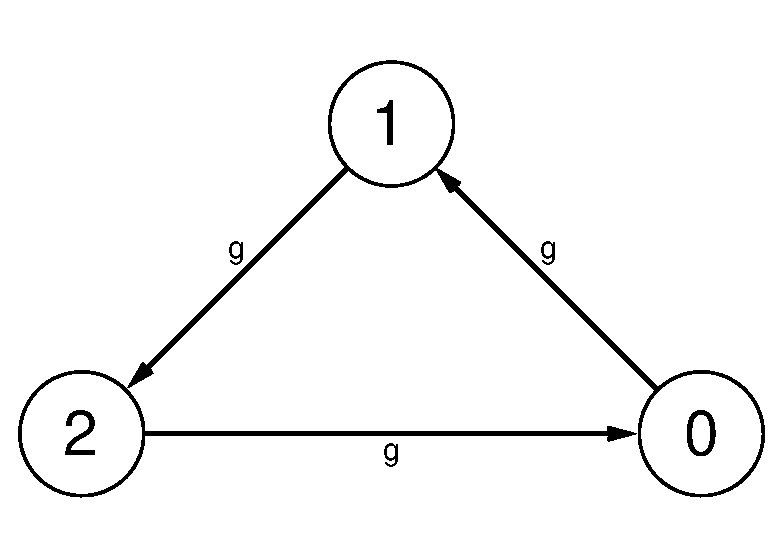
\includegraphics[width=0.35\textwidth]{fig/taxas.eps}}
\caption{\label{fig:taxas}
    Transition rates for an isolated unit.
    }
\end{center}
\end{figure}

\begin{figure}
    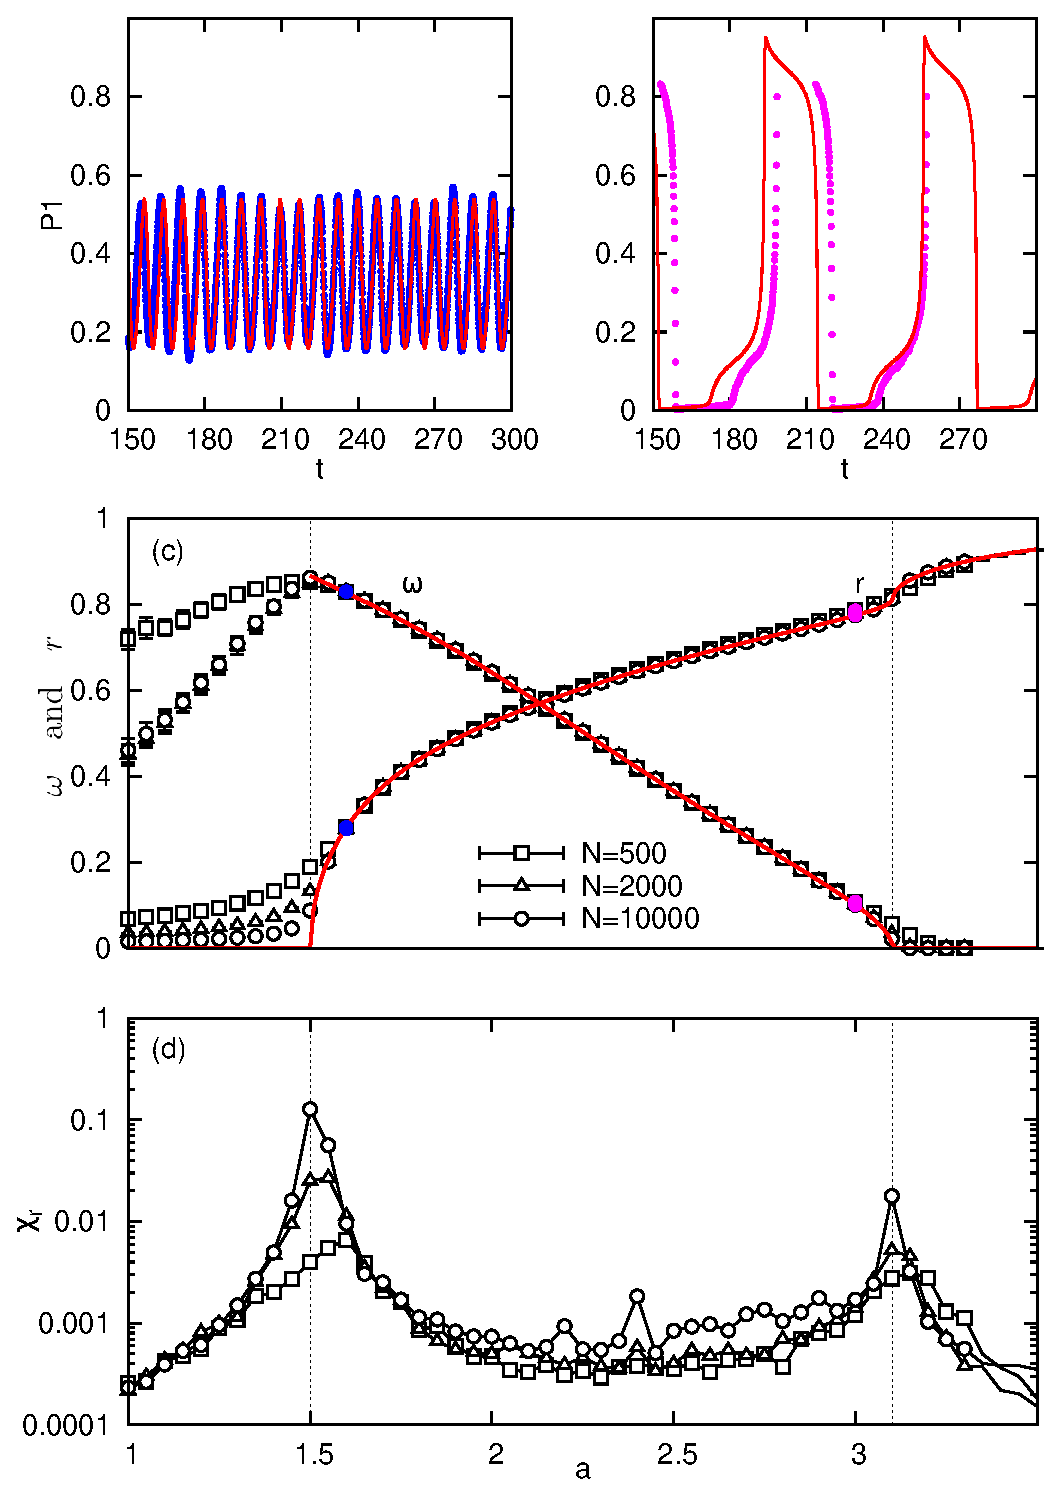
\includegraphics[height=.75\textheight]{fig/figure2.eps}
\begin{center}
\caption{\label{complete_graph} (Color online) Panels (a) and (b) show the evolution of $P_1$ for $a=1.6$ and $a=3$, respectively.
Points: simulations of a complete graph of $N$ nodes; lines: MF solution. (c) Dependence of $r$ and $\omega$ on $a$, exhibiting the two
phase transitions. (d) $\chi_r$ versus $a$, showing peaks at the transitions [system sizes as in (c)].  }
\end{center}
\end{figure}

In the WCM, the state $s^x$ at site $x$ ($x=1,\ldots,N$) can take one of three values, $s^x \in \{0,1,2\}$, corresponding to a phase
$\phi^x = 2 \pi s_x/3$.  The only allowed transitions are those from $s$ to $s+1$ (modulo 3) (see Fig.~\ref{fig:taxas}), which implies
that detailed balance is violated. If site $x$ is in state $s^x=j$, its transition rate to state $j+1$ is:

\begin{equation}
\label{eq:gj}
\gamma^x_j = g \exp \left[ a\frac {\left( n^x_{j+1} - n^x_j \right)} {n^x} \right]
\end{equation}

\noindent where $g$ is a constant, $a$ is the coupling parameter, $n^x_j$ is the number of neighbors of site $x$ in state $j$, and
$n^x$ is the number of neighbors for site $x$. Since these rates are invariant under cyclic permutation of the state indices, the model
is invariant under the group $C_3$ of discrete rotations.

Let $N_j$ be the total number of sites in state $j$, so that $N_0 +N_1 +N_2 = N$, the total number of sites. As discussed in
\cite{assis2011infinite}, the MF approximation, obtained by replacing $n^x_j/n^x$ in the argument of the exponential
of~Eq.(\ref{eq:gj}) with the corresponding state fraction, $n_j = N_j/N$, yields three non equilibrium phases, separated by two
continuous phase transitions. For small coupling ($a < a_c = 1.5$), the disordered phase, with $\textbf{n}=(1/3,1/3,1/3) \equiv
\textbf{n}_{1/3}$, is the stable stationary solution of the MF equations. ($\textbf{n}$ denotes the vector of state fractions.) For $a$
between $a_c$ and a higher value, $a^c\simeq 3.102\, 439\, 915\, 64$, there is no stable stationary solution and the MF equations admit
an oscillatory solution (a limit cycle) in which states 0, 1 and 2 periodically assume the role of the majority. As $a$ is increased
above $a_c$, the frequency $\omega$ of oscillation decreases continuously, becoming zero at $a^c$, signalling the IP transition.  For
$a> a^c$, three stationary solutions, \textbf{n}$_j$ appear, such that state $j$ represents the (permanent) majority. Thus $C_3$
symmetry is broken for $a > a^c$. (The three solutions are, naturally, related via cyclic permutation of indices in state space.) 

The WCM is characterized by a pair of order parameters. First, one has the familiar Kuramoto synchronization parameter
~\cite{Kuramoto84,Strogatz00,Wood06a},

\begin{equation}
    r \equiv \left<\left< |v| \right>_t\right>_s,
    \label{eq:r}
\end{equation}
\noindent where
\begin{equation}
    v \equiv \frac{1}{N} \sum^{N}_{x=1} e^{i\phi^x}.
    \label{eq:v}
\end{equation} 

\noindent In Eq.~(\ref{eq:r}),  $\left< \right>_t$ denotes a time average over a single realization (in the stationary state), and
$\left< \right>_s$ an average over independent realizations. Note that $r > 0$ is consistent with, but does not necessarily imply,
globally synchronized oscillation. The latter is characterized by a periodically varying phase of
$v$~\cite{Kuramoto92a,Ohta08,ShinomotoKuramoto86,Rozenblit11}.

In the MF analysis, the transition to the synchronized regime (the GO transition) is associated with a supercritical Hopf bifurcation
at $a=a_c=1.5$: the trivial fixed point $\textbf{n}_{1/3}$ loses stability at $a=a_c$, and a limit cycle encircling this point appears.
For $a \gtrsim a_c$, sustained oscillations in $n_j$ characterize synchronization among the oscillators (Fig.~\ref{complete_graph}a).
Correspondingly, $r$ grows continuously $\sim (a-a_c)^\beta$ at the transition (Fig.~\ref{complete_graph}c), with a MF exponent $\beta
= 1/2$~\cite{Wood06a}. The scaled variance

\begin{equation}
    \chi_r \equiv L^d \left[ \left< \left< |v| \right>^2_t \right>_s - r^2 \right],
    \label{eq:chir}
\end{equation}

\noindent diverges with the system size at criticality, as shown in Fig.~\ref{complete_graph}d for simulations on the complete graph
\cite{assis2011infinite}. The GO transition is associated with breaking of the continuous time-translation symmetry: the
$\textbf{n}_k(t)$, are periodic for $a\gtrsim a_c$.  Increasing $a$ above $a_c$ enhances synchronization among the oscillators, leading
to increasing oscillation amplitudes, as shown in Fig.~\ref{complete_graph}b.

Wood \textit{et al.} found that the increasing amplitude of oscillation is accompanied by a decreasing angular frequency $\omega =
2\pi/\langle \tau \rangle$, where $\langle \tau \rangle$ is the mean time between peaks in $n_k$ (Figs.~\ref{complete_graph}a-c). This
can be understood qualitatively from the exponential dependence of the transition rates of Eq.~(\ref{eq:gj}) on the neighbor fractions:
When a state is highly populated, the rate at which oscillators leave it becomes very small.  In the MF theory, when $a$ reaches the
upper critical value $a^c$, three symmetric saddle-node bifurcations occur simultaneously, and the period of the collective
oscillations diverges \cite{assis2011infinite}. Above $a^c$, there are three symmetric attractors in the system, and 3-fold rotational
($C_3$) symmetry is spontaneously broken.  As in condensation or a ferromagnetic phase transition~\cite{Huang}, freezing of the
majority state does not imply that individual oscillators freeze as well.  The transition rates of individual oscillators do decrease
with increasing $a$, but only vanish in the limit $a\to\infty$, when one of the states is fully occupied.

It is convenient to define an order parameter $\psi$ that is identically zero (in the infinite-size limit) for $a>a^c$. Assis et al.
proposed \cite{assis2011infinite},
\vspace{1em}

\begin{equation}
    \label{eq:psi}
    |\psi| \equiv \frac{1}{N}\left| \sum_{x=1}^N \left( \delta_{0,s^x} + e^{2\pi i/3}\delta_{1,s^x} + e^{-2\pi i/3}\delta_{2,s^x} \right) \gamma^x \right|
\end{equation}
\vspace{1em}

\noindent where $\delta_{ij}$ is the Kronecker delta and $\gamma^x \equiv \gamma^x_{s^x}$ is the transition rate at site $x$ (see
eq.~\ref{eq:gj}). Thus $|\psi|$ involves not only the configuration, but the rate at which the latter evolves.  On the complete graph,
$\gamma^x$ is the same for all sites $x$ in the same state $j$. Denoting this rate by $\gamma_j$, the order parameter can be written
(in MF analysis) as

\begin{equation}
    \label{eq:psiMF}
    |\psi|^2 \stackrel{MF}{=} \sum_{j=0}^2 (n_j \gamma_j - n_{j-1} \gamma_{j-1})^2 
\end{equation}

\noindent Both the disordered phase ($a< a_c$) as well as the IP phase ($a>a^c$) have stable, stationary solutions, $\textbf{n}^*$.
Since $\dot{n}_j = 0$ implies $n^*_j\gamma_j = n^*_{j-1}\gamma_{j-1}$, i.e., zero net change in the probability of state $j$, we have
$|\psi|=0$ in eq.~\ref{eq:psiMF} for both cases [a similar line of reasoning can be applied directly to Eq.~(\ref{eq:psi})].

\begin{figure}
\begin{center}
    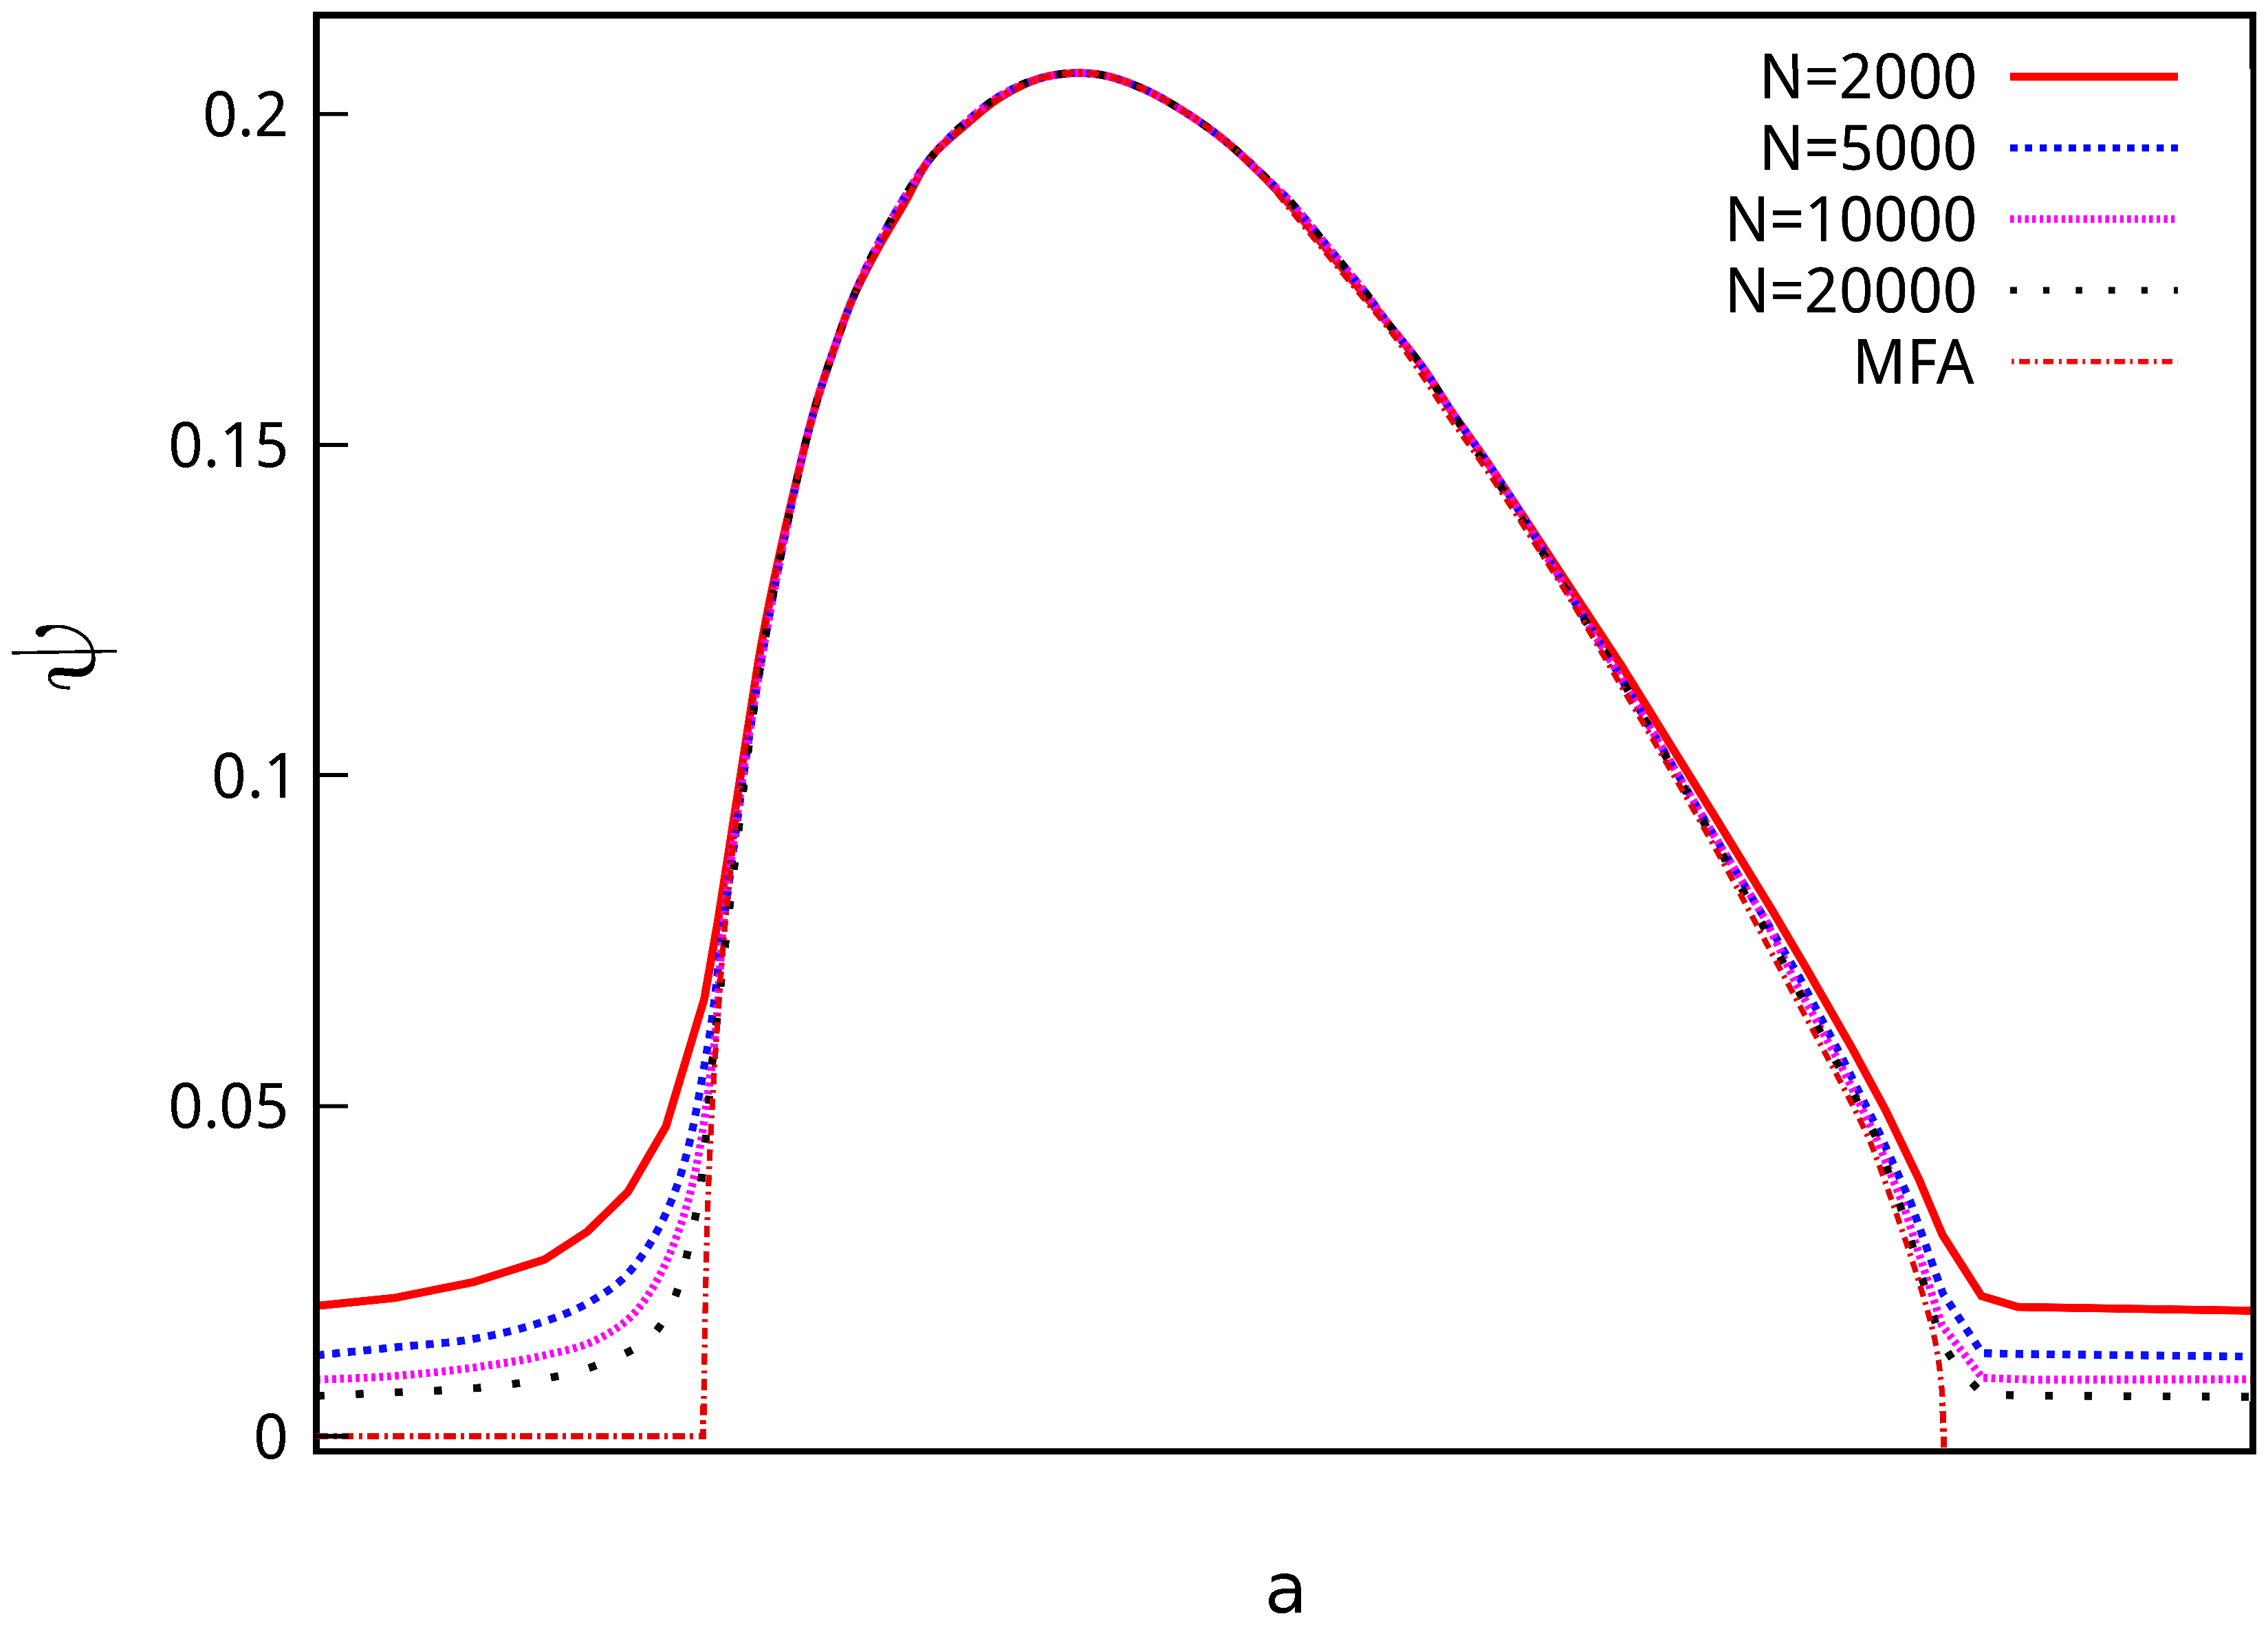
\includegraphics[width=0.7\textwidth]{fig/psivsa.eps}
    \caption{\label{fig:psi}
        (Color online) (From \cite{assis2011infinite}.) Order parameter $\langle
        |\psi| \rangle$ as a function of coupling $a$ in the MF theory and
        on the complete graph, for sizes as indicated.
    }
\end{center}
\end{figure}

Figure \ref{fig:psi} shows $\langle |\psi| \rangle$ versus $a$ in MF theory, and on the complete graph (the latter via numerically
exact solution of the master equation), confirming that $|\psi|$ functions as an order parameter to detect both the GO and IP phase
transitions. The MF critical behavior is $\langle |\psi| \rangle \sim (a- a_c)^{1/2} $ for $a \searrow a_c$ and $\langle |\psi| \rangle
\sim (a^c - a)^{1/2}$ for $a \nearrow a^c$.  On the complete graph, the order parameter decays with system size as $\langle |\psi|
\rangle \sim N^{-1/4}$ at $a=a_c$ and as $N^{-0.4203(3)}$ at $a=a^c$. The first result is typical of MF scaling with system size at a
continuous phase transition, as argued in \cite{assis2011infinite}.

The results for the IP transition in MF and on a complete graph are in sharp contrast to what is found on finite-dimensional lattices.
The \textit{absence} of such a transition was verified numerically on hyper cubic lattices in dimensions $d \leq 4$ in
\cite{assis2011infinite}. This reference also provides a quantitative argument showing that on finite-dimensional lattices, a $j$-state
majority cannot persist indefinitely: it is always susceptible to change via nucleation of a cluster of state $j+1$. The authors of
\cite{assis2011infinite} conjectured that the IP transition would occur on structures in which a site interacts with a nonzero fraction
of all other sites (as the system size tends to infinity). In the following sections we test this conjecture on two structures, regular
rings with extended interactions, and small-world networks.

\section{\label{regularrings} The WCM on regular rings }


A \textit{regular ring} is constructed starting from a graph of $N$ nodes arranged in circular fashion. Considering one node at a time in
a clockwise manner, we connect it to its $K$ nearest neighbors in the clockwise direction; an example of such a structure is shown in
Fig.~\ref{fig:ring}. We define the \textit{connectivity} of a regular ring graph by $\alpha \equiv K/N$, such that $\alpha=1/N$ signifies
a one-dimensional chain while $\alpha=0.5$ represents a complete graph. Thus, one can interpolate from the one-dimensional to an
infinite-dimensional hyper cubic lattice (complete graph) varying $\alpha$ over the interval $\left( 0, \frac{1}{2} \right]$.  It is
known that the WCM on hyper cubic lattices of dimensions 1 and 2 cannot sustain ordered phases \cite{Wood06a, assis2011infinite}. Since
$\alpha=0.5$ represents the complete graph, there must be at least one threshold $\alpha=\alpha^*$ above which one or both phase
transitions (GO and IP) occur, varying $a$.

Different from hyper cubic lattices, in which coupling is local, for $\alpha > 0$ the coupling on ring graphs is nonlocal.  The manner
in which the interaction range scales as $N\to\infty$ can be chosen in different ways; the simplest, which we consider here, is to fix
$\alpha$ so that $K \propto N$ (More precisely,  $K=\lceil\alpha N\rceil$ where $\lceil x \rceil$ denotes the smallest integer larger
than $x$).  It is reasonable to expect that phase transitions occur for any fixed $\alpha > 0$, since the interaction range $K$ then
tends to infinity with $N$. 

\begin{figure}[b]
\begin{center}
    \fbox{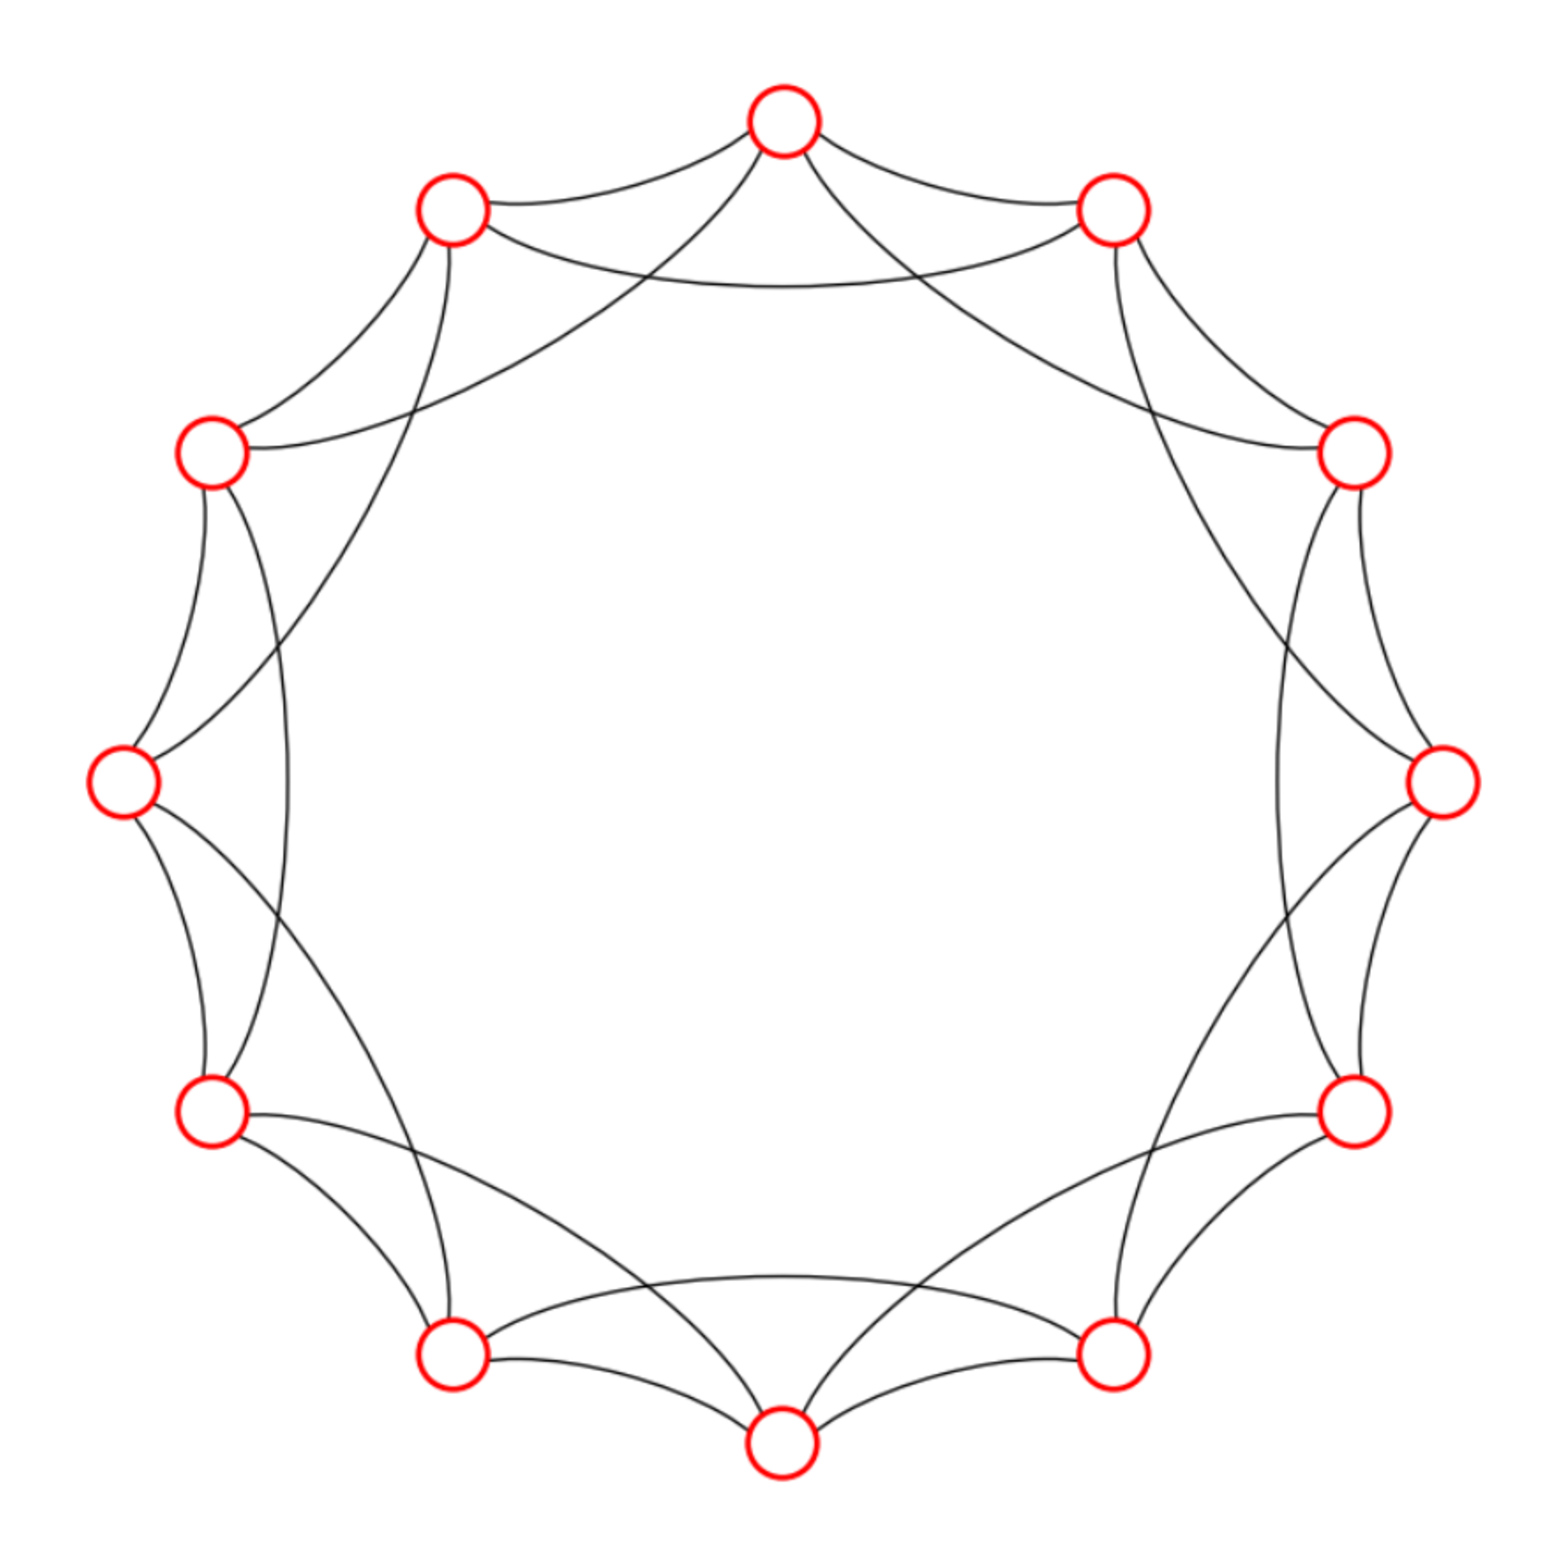
\includegraphics[width=0.40\textwidth]{fig/ring.eps}}
\caption{\label{fig:ring}
    A regular ring is an undirected graph with $N$ nodes arranged in circular
    fashion, with each connected to its $K$ nearest neighbors in each direction.
    Here we show an example with $N=12$ and $K=2$.
    }
\end{center}
\end{figure}

\begin{figure}[t]
\begin{center}
    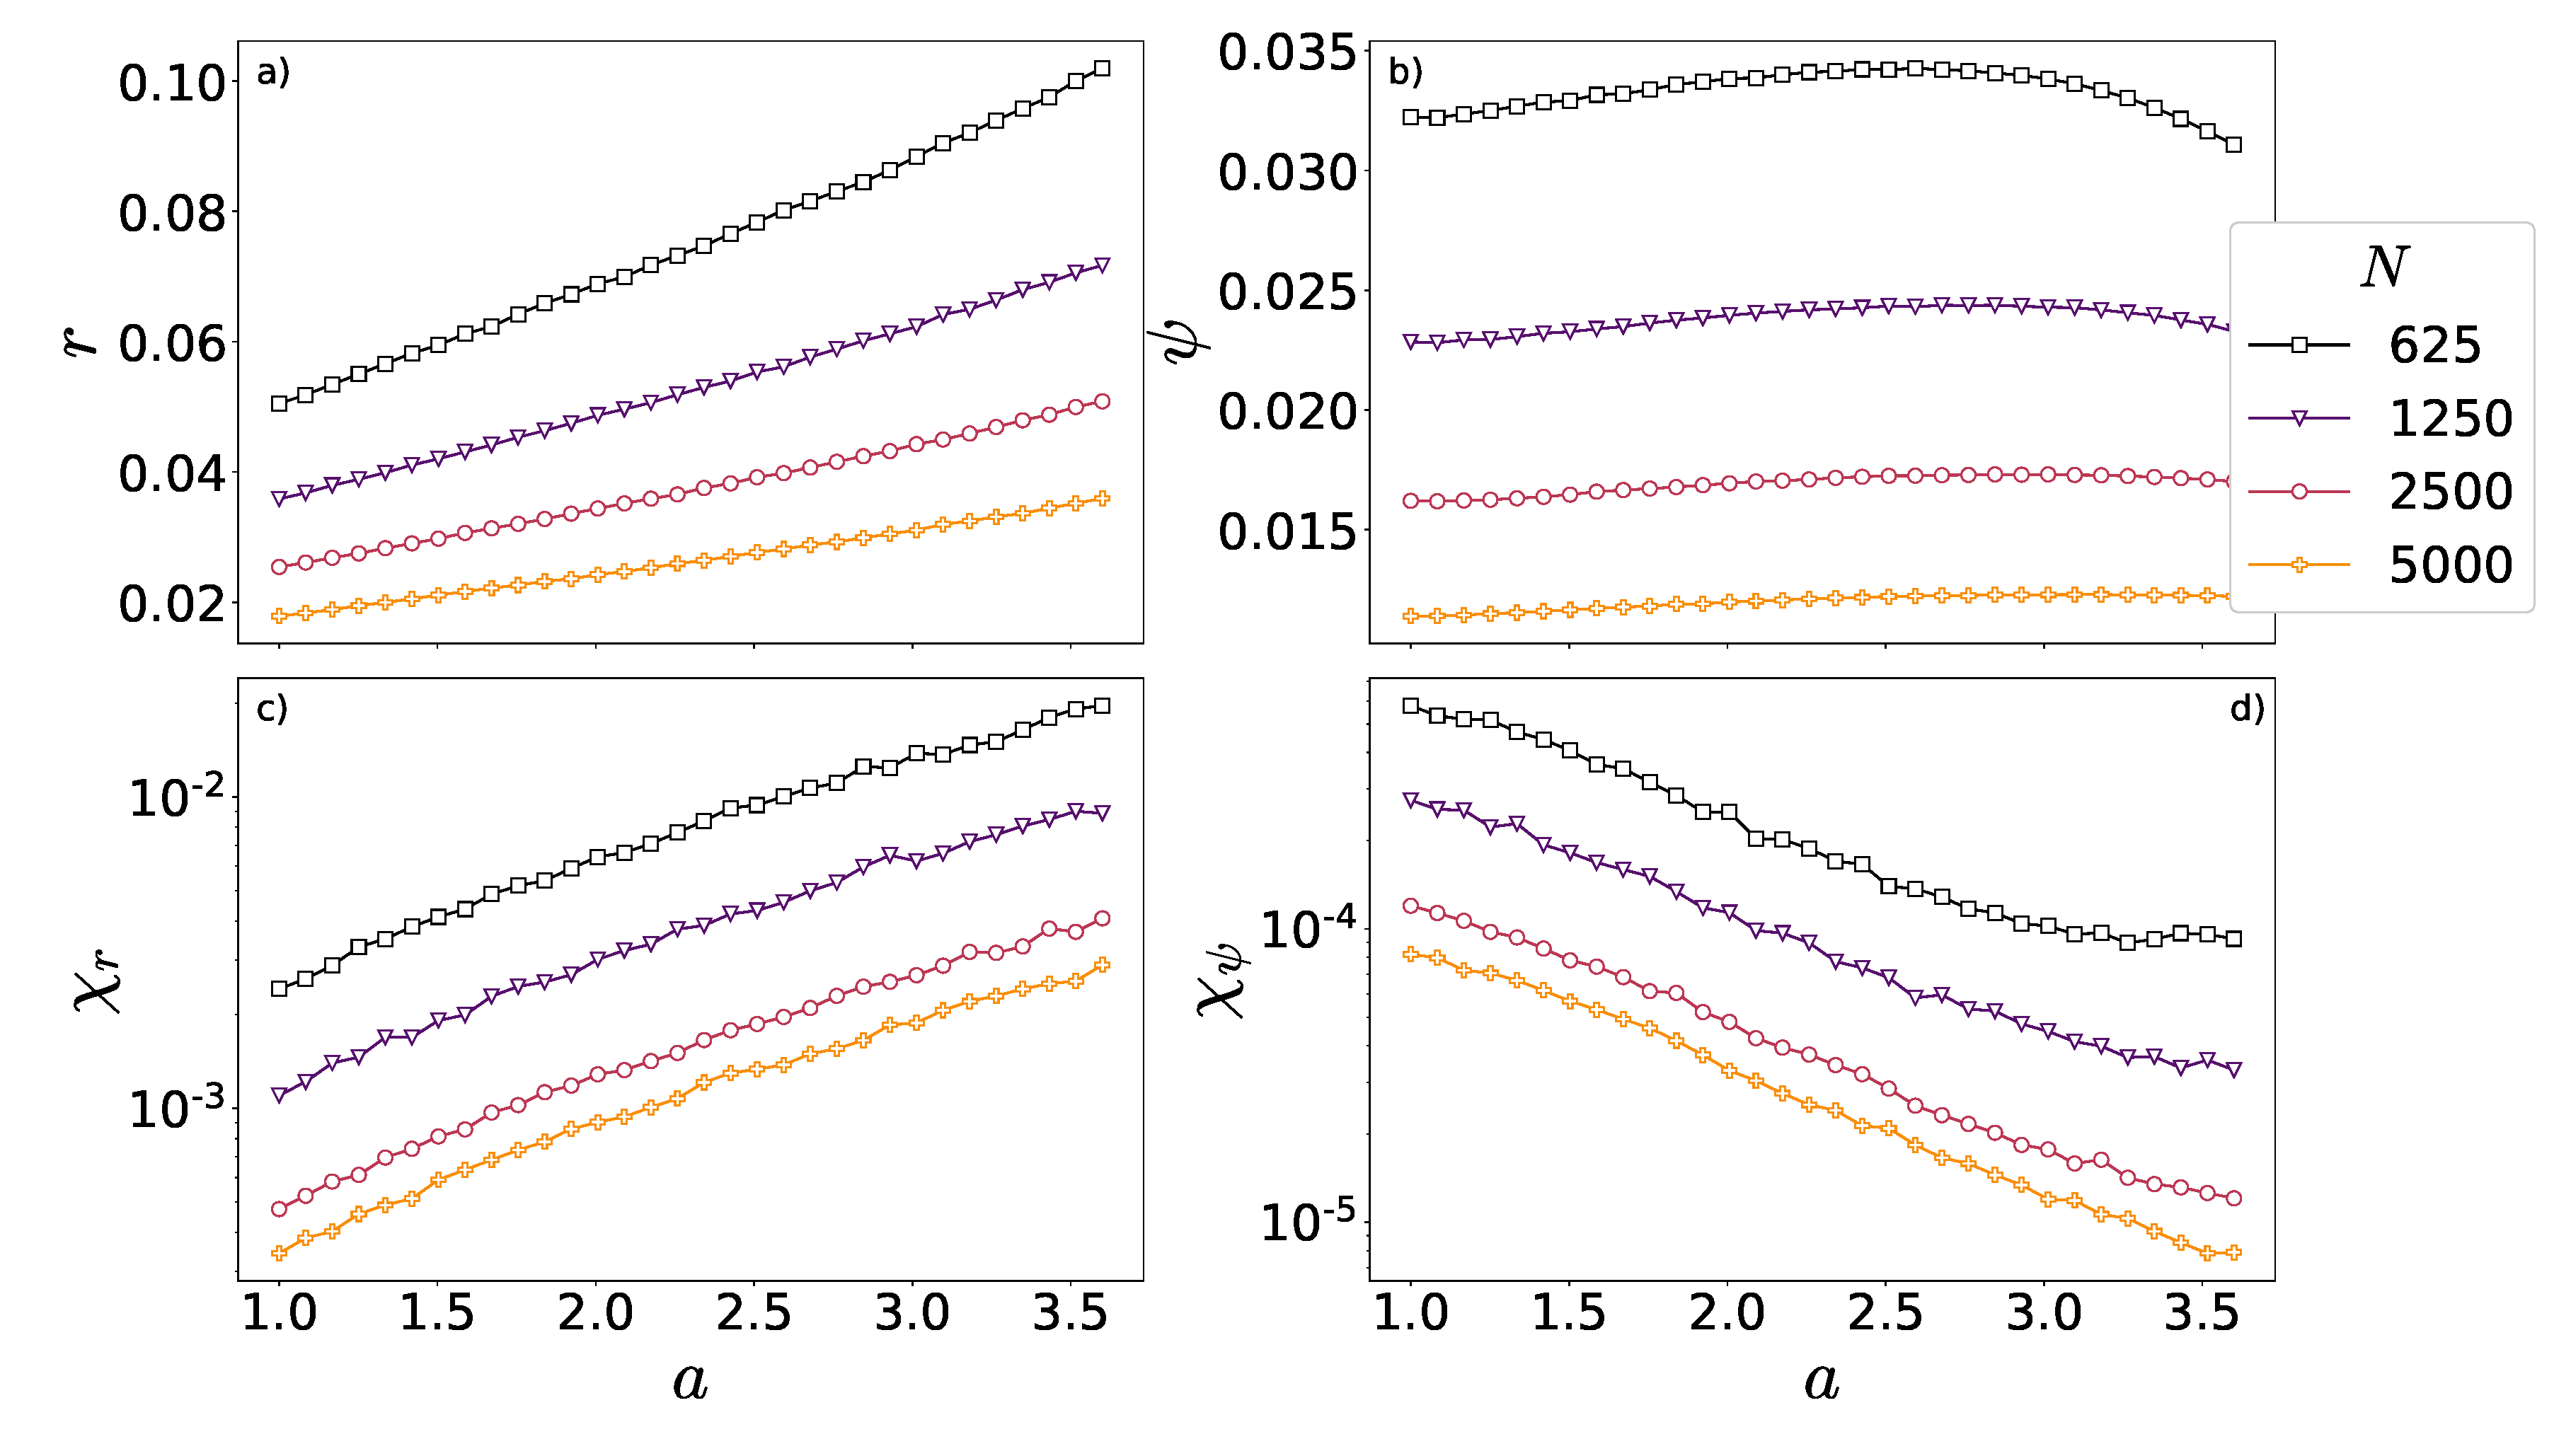
\includegraphics[width=0.9\textwidth]{fig/chi_curves_1D.eps}
\caption{\label{fig:chi_curves_1D}
    (Color online) Order parameters and their scaled variances for
    one-dimensional rings ($K=1$). Both the order parameters and their
    respective variances decrease as the system size is increased, with $r
    \approx \psi \approx 0$ across a wide range of coupling strengths. Points
    represent an average over 3000 independent realizations with random initial
    configurations. For the 1D chain, the same behavior is observed regardless
    of initial configuration.
    }
\end{center}
\end{figure}

\begin{figure}[t]
\begin{center}
    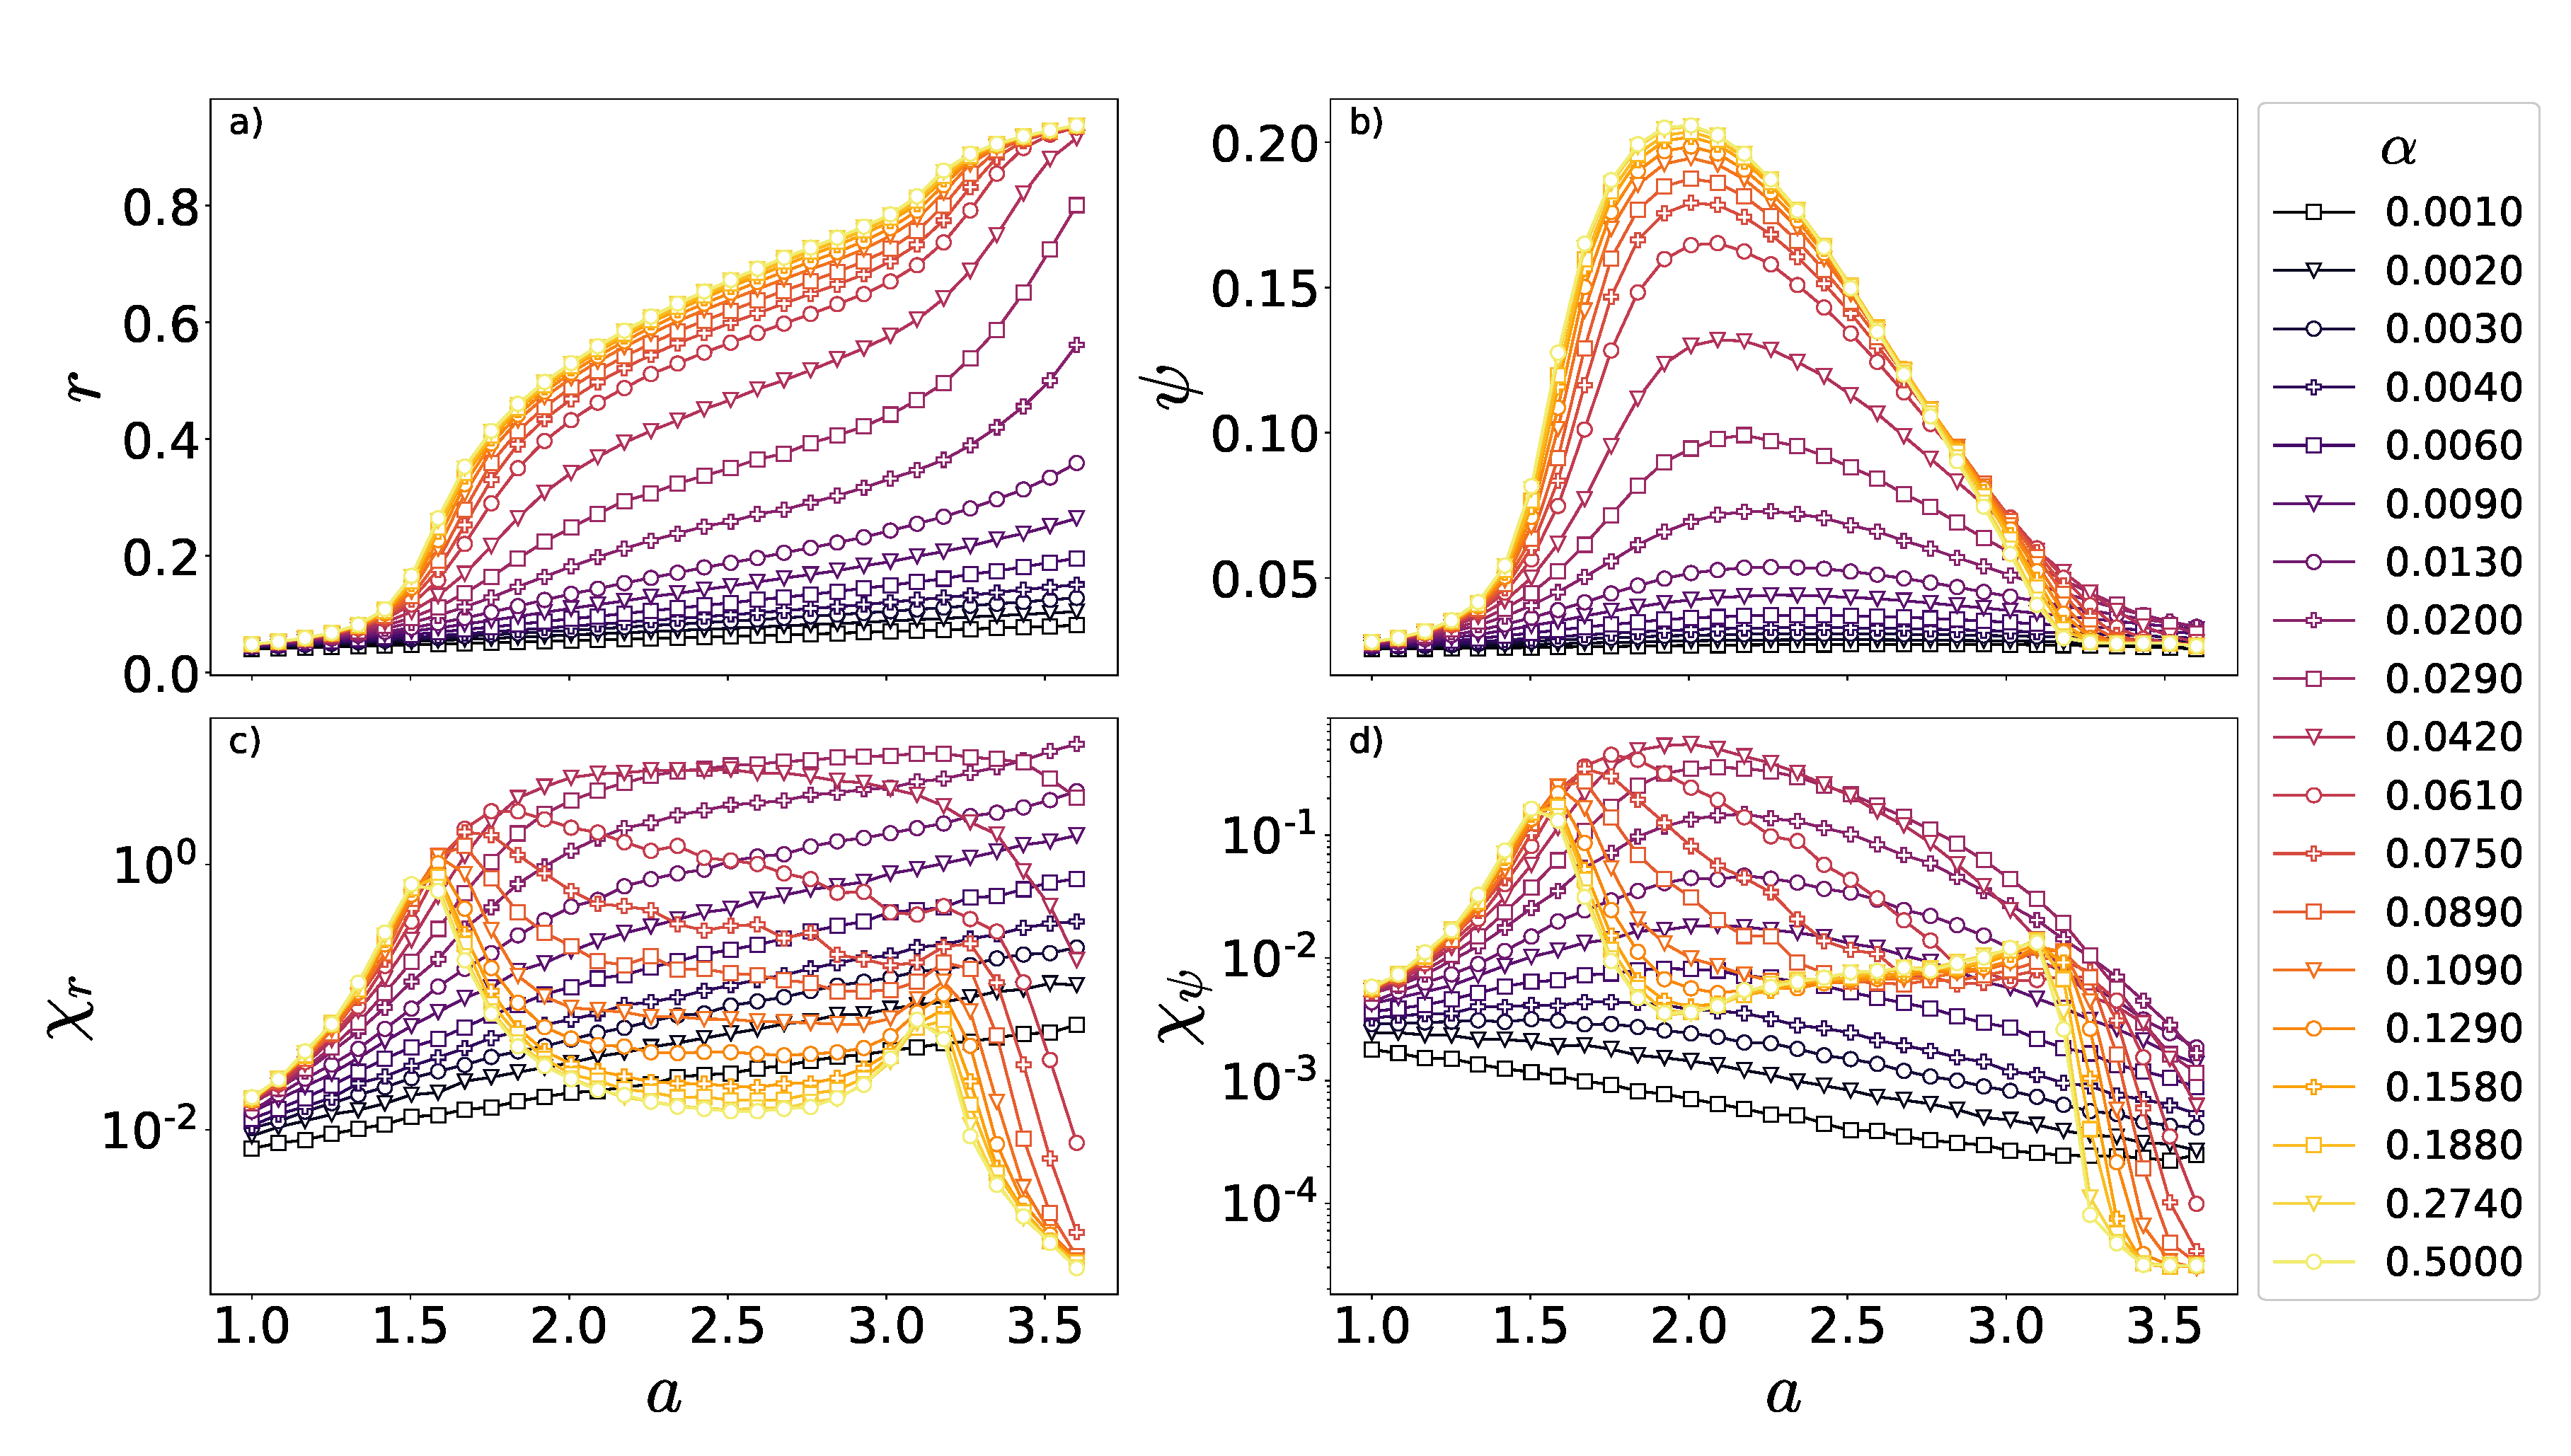
\includegraphics[width=0.95\textwidth]{fig/chi_curves_uniformic.eps}
    \caption{\label{fig:chicurves}
    (Color online) Order parameters and scaled variances for regular rings of
    size $N=1000$ and various values of the connectivity $\alpha$.  Points
    represent an average over 4000 independent realizations with uniform initial
    configurations.
    }
\end{center}
\end{figure}

\subsection{Scaling behavior: phase boundary}

The dynamics as $N$ increases can be studied by defining the scaled variances of the order parameters. These quantities are expected to
diverge in the thermodynamic limit when the system undergoes a continuous phase transition \cite{plischke1994equilibrium}.  The scaled
variances of order parameters $r$ and $\psi$ can be defined through equations \ref{eq:v} and \ref{eq:psi} as:

\begin{align}
    \chi_r &= \chirdef \notag , \\
    \chi_\psi &= \chipsidef,
\end{align}

\noindent where $\left<\right>_t$ and $\left<\right>_s$ are averages over time and over independent realizations, respectively.

In simulations, the system is allowed to relax to a steady state, starting from its initial configuration.  Once the steady state has
been attained, the order parameters are averaged over the remainder of the evolution. As we will see, the choice of initial condition
is important for some values of the interaction range $K$; we will focus on two different setups: \textit{random} initial
configurations, in which the initial phase of each oscillator is chosen uniformly and independently among the three possible values in
$\{ 0, 2\pi/3, 4\pi/3 \}$, and a \textit{uniform} initial condition, in which $\phi_i = 0, \; \forall i$.

In the following we describe results for uniform initial conditions. In Fig.~\ref{fig:chi_curves_1D} we plot the order parameters and
their associated variances for $K=1$ (i.e.,  $\alpha=1/N$). Both quantities are shown to decrease with system size (for the 1D case in
particular this behavior is the same regardless of initial configuration), indicating the absence of phase transitions. In
Fig.~\ref{fig:chicurves}, the same quantities are shown for regular rings with $N=1000$ and various $\alpha$ values.  As expected, the
order parameters and their variances approach the complete-graph limit as $\alpha$ nears the value $1/2$.  Denoting by $\alpha^*$ the
value associated with a change from one to two maxima in $\chi_{\psi}$, we identify $\alpha^* \approx 0.06$ for $N=1000$ in
Fig.~\ref{fig:chicurves}.  Performing similar analyses for different system sizes we obtain $\alpha^*$ as a function of $N$.  To infer
the scaling behavior, we define $\lambda \equiv N^{-1}$ and look at the $\alpha^*$ versus $\sqrt{\lambda}$ curve near $\lambda=0$. The
resulting data, shown in Fig.~\ref{fig:alphasplit}, suggest that $\alpha^*$ tends to zero as $N\to\infty$. This supports the conjecture
stated previously that in this limit, and for any fixed $\alpha>0$, the WCM on a regular ring lattice exhibits both GO and IP phase
transitions.

\begin{figure}
\begin{center}
    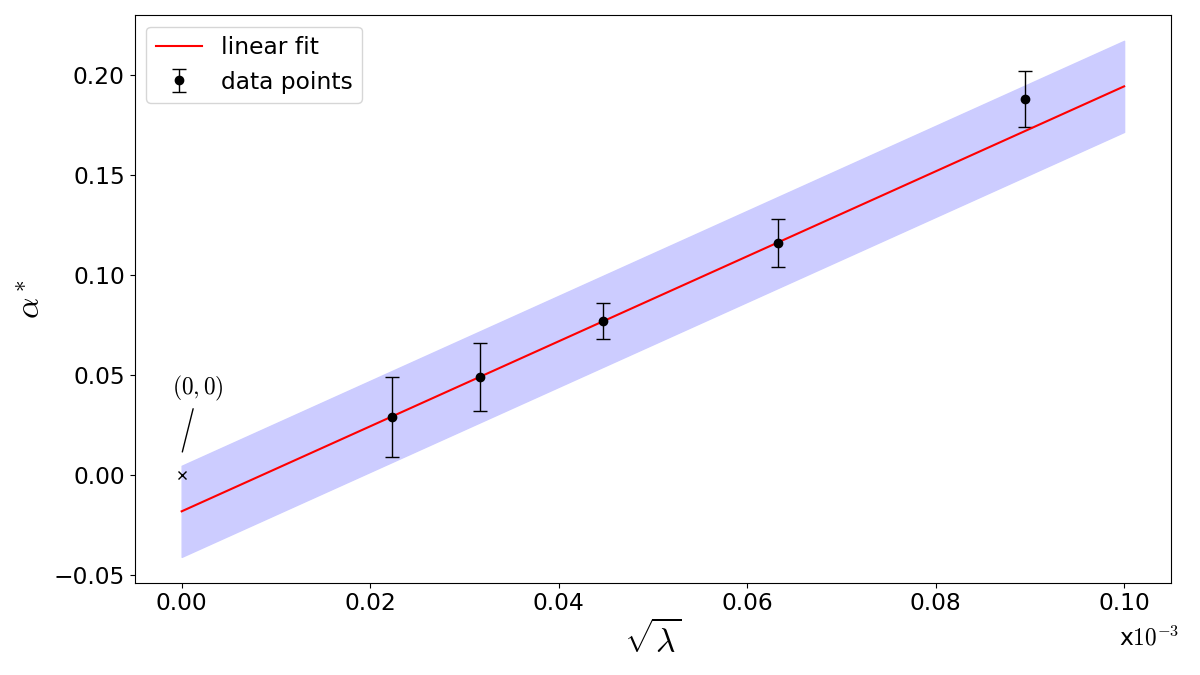
\includegraphics[width=0.9\textwidth]{fig/alphasplit.png}
    \caption{\label{fig:alphasplit} Plot of $\alpha^*$ versus $\sqrt{\lambda}$. Starting from uniform initial configurations, $\alpha >
        \alpha^*$ means $\chi_{\psi}$ and $\chi_r$ exhibit two maxima, whereas for $\alpha < \alpha^*$ only a single broad maximum is
        observed. Full circles represent data obtained from simulations and solid curve is a linear fit with equation
        $y=-0.01837+2.1271x$. The band around the fitted curve represent the uncertainty associated with the linear intercept.}
\end{center}
\end{figure}

\subsection{Scaling behavior: order parameter}

To better understand the scaling behavior we look at the order parameters as $N \to \infty$ with fixed $\alpha$. If both $r$ and $\psi$
tend to zero, there is no global synchronization. Both order parameters tending to positive values indicates the presence of global or
intermittent synchronization among large populations of oscillators, while $\psi \to 0$ with $r \sim 1$ defines an infinite-period
phase.

\begin{figure}
\begin{center}
    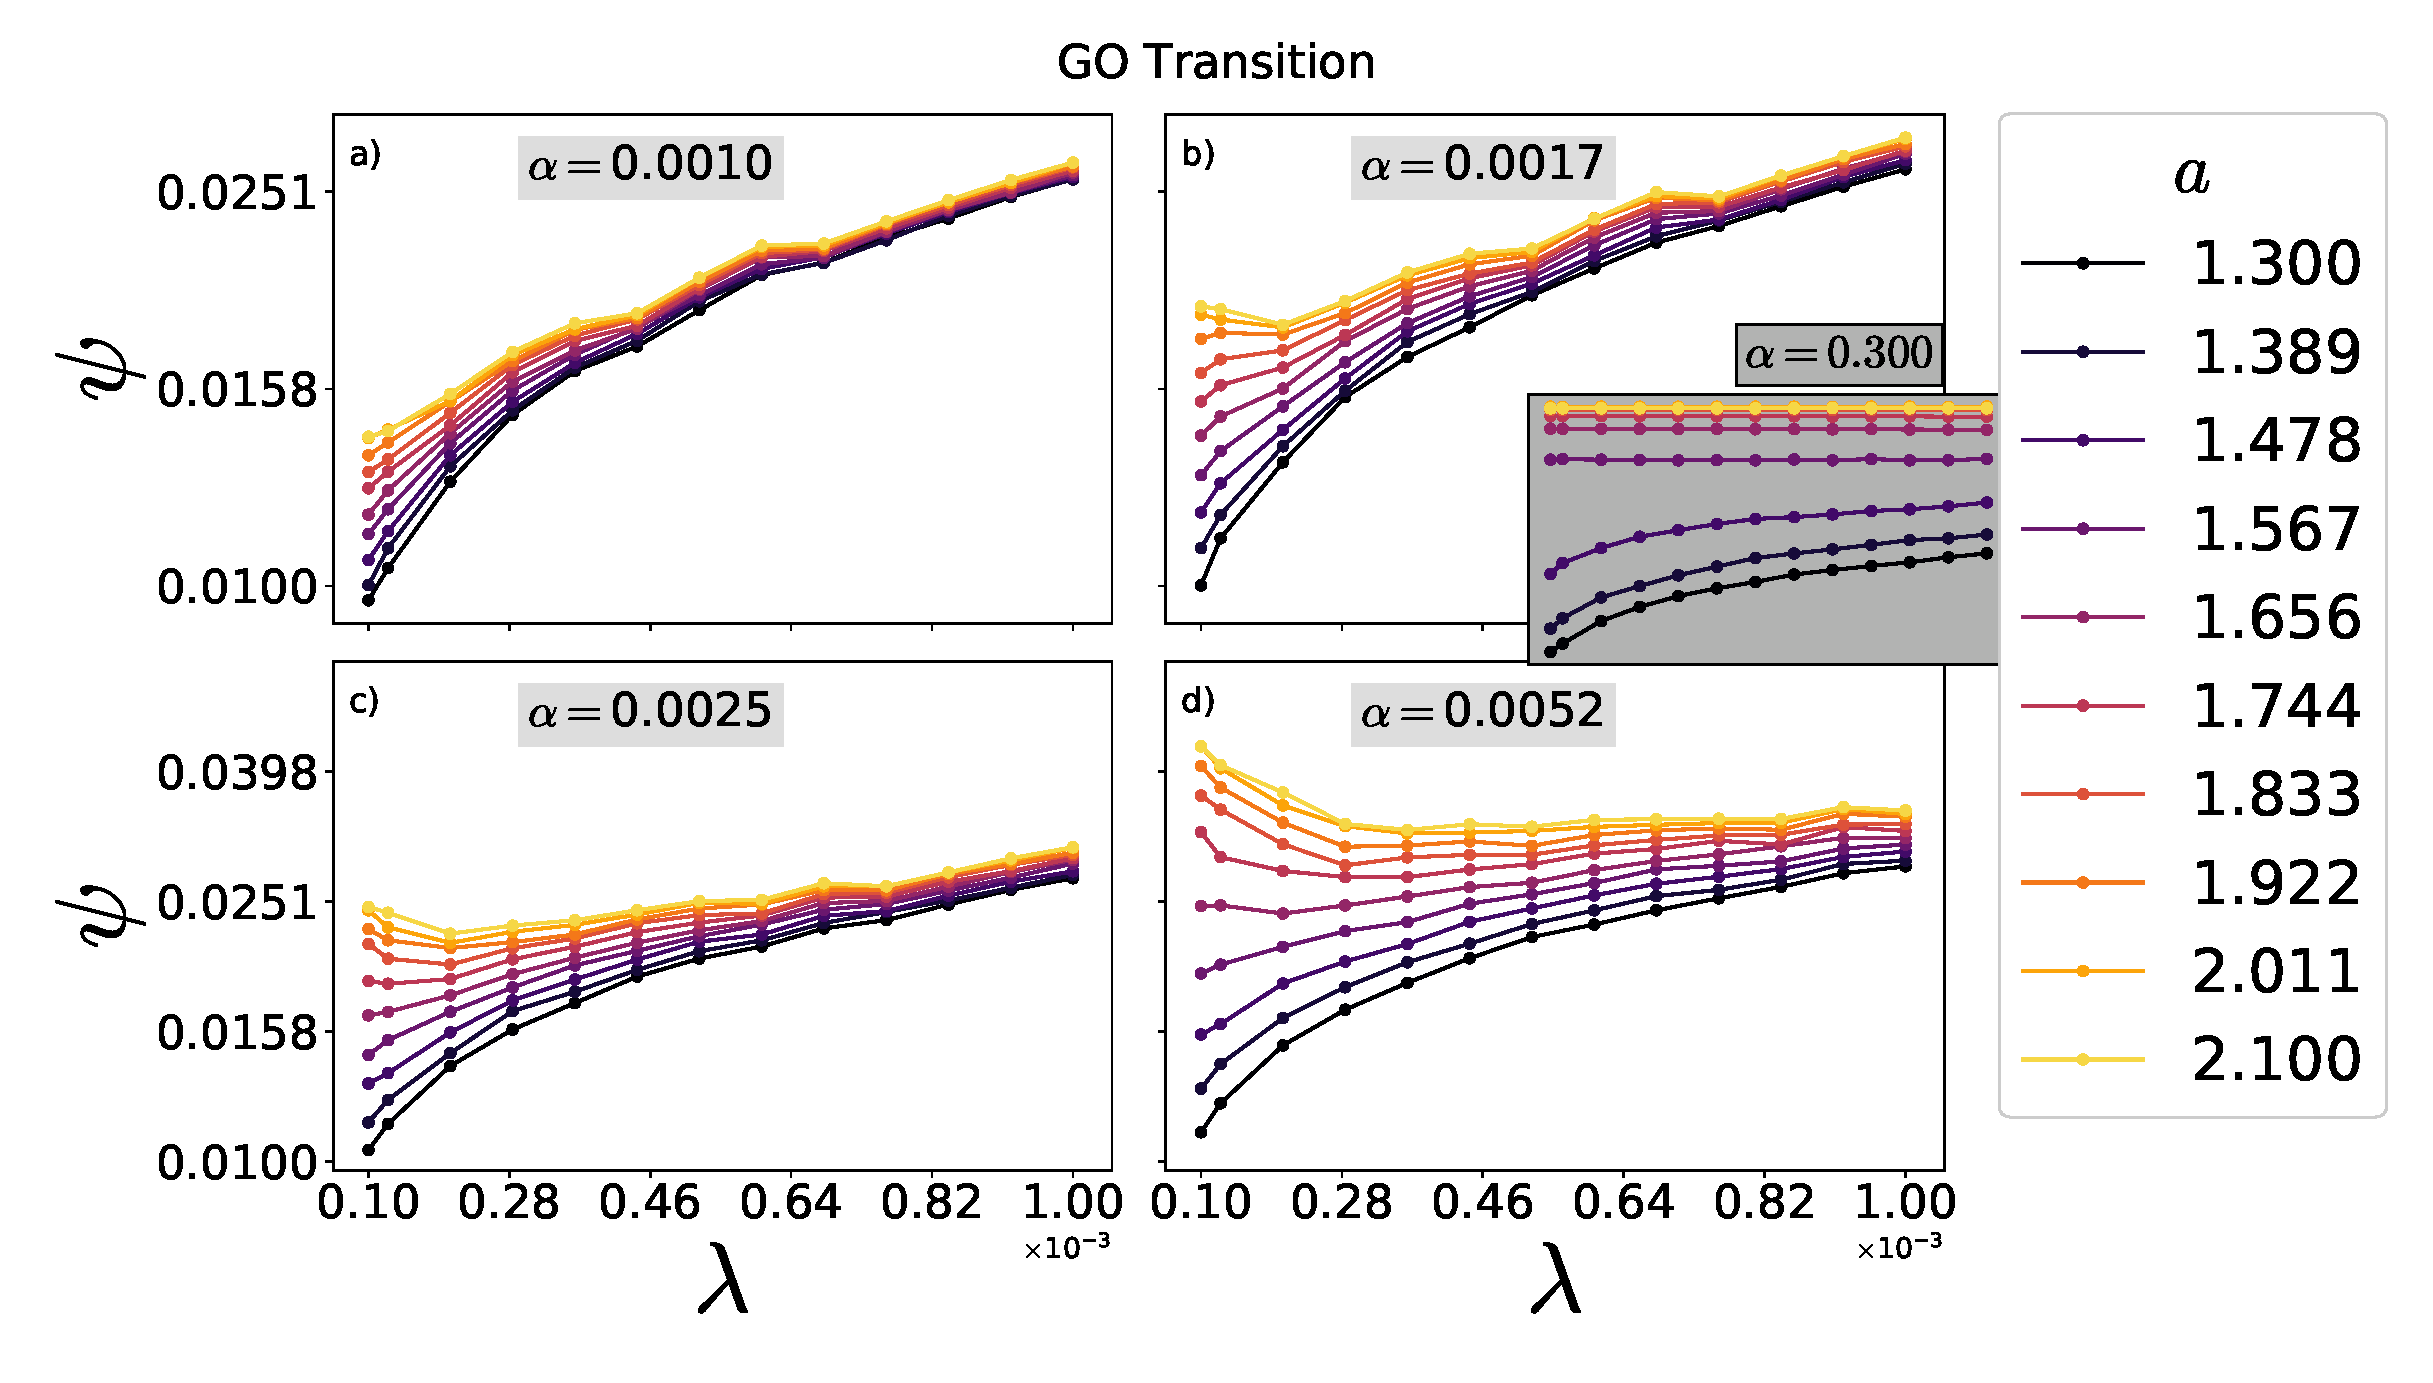
\includegraphics[width=0.85\linewidth]{fig/opsplit-psi-got.eps}
    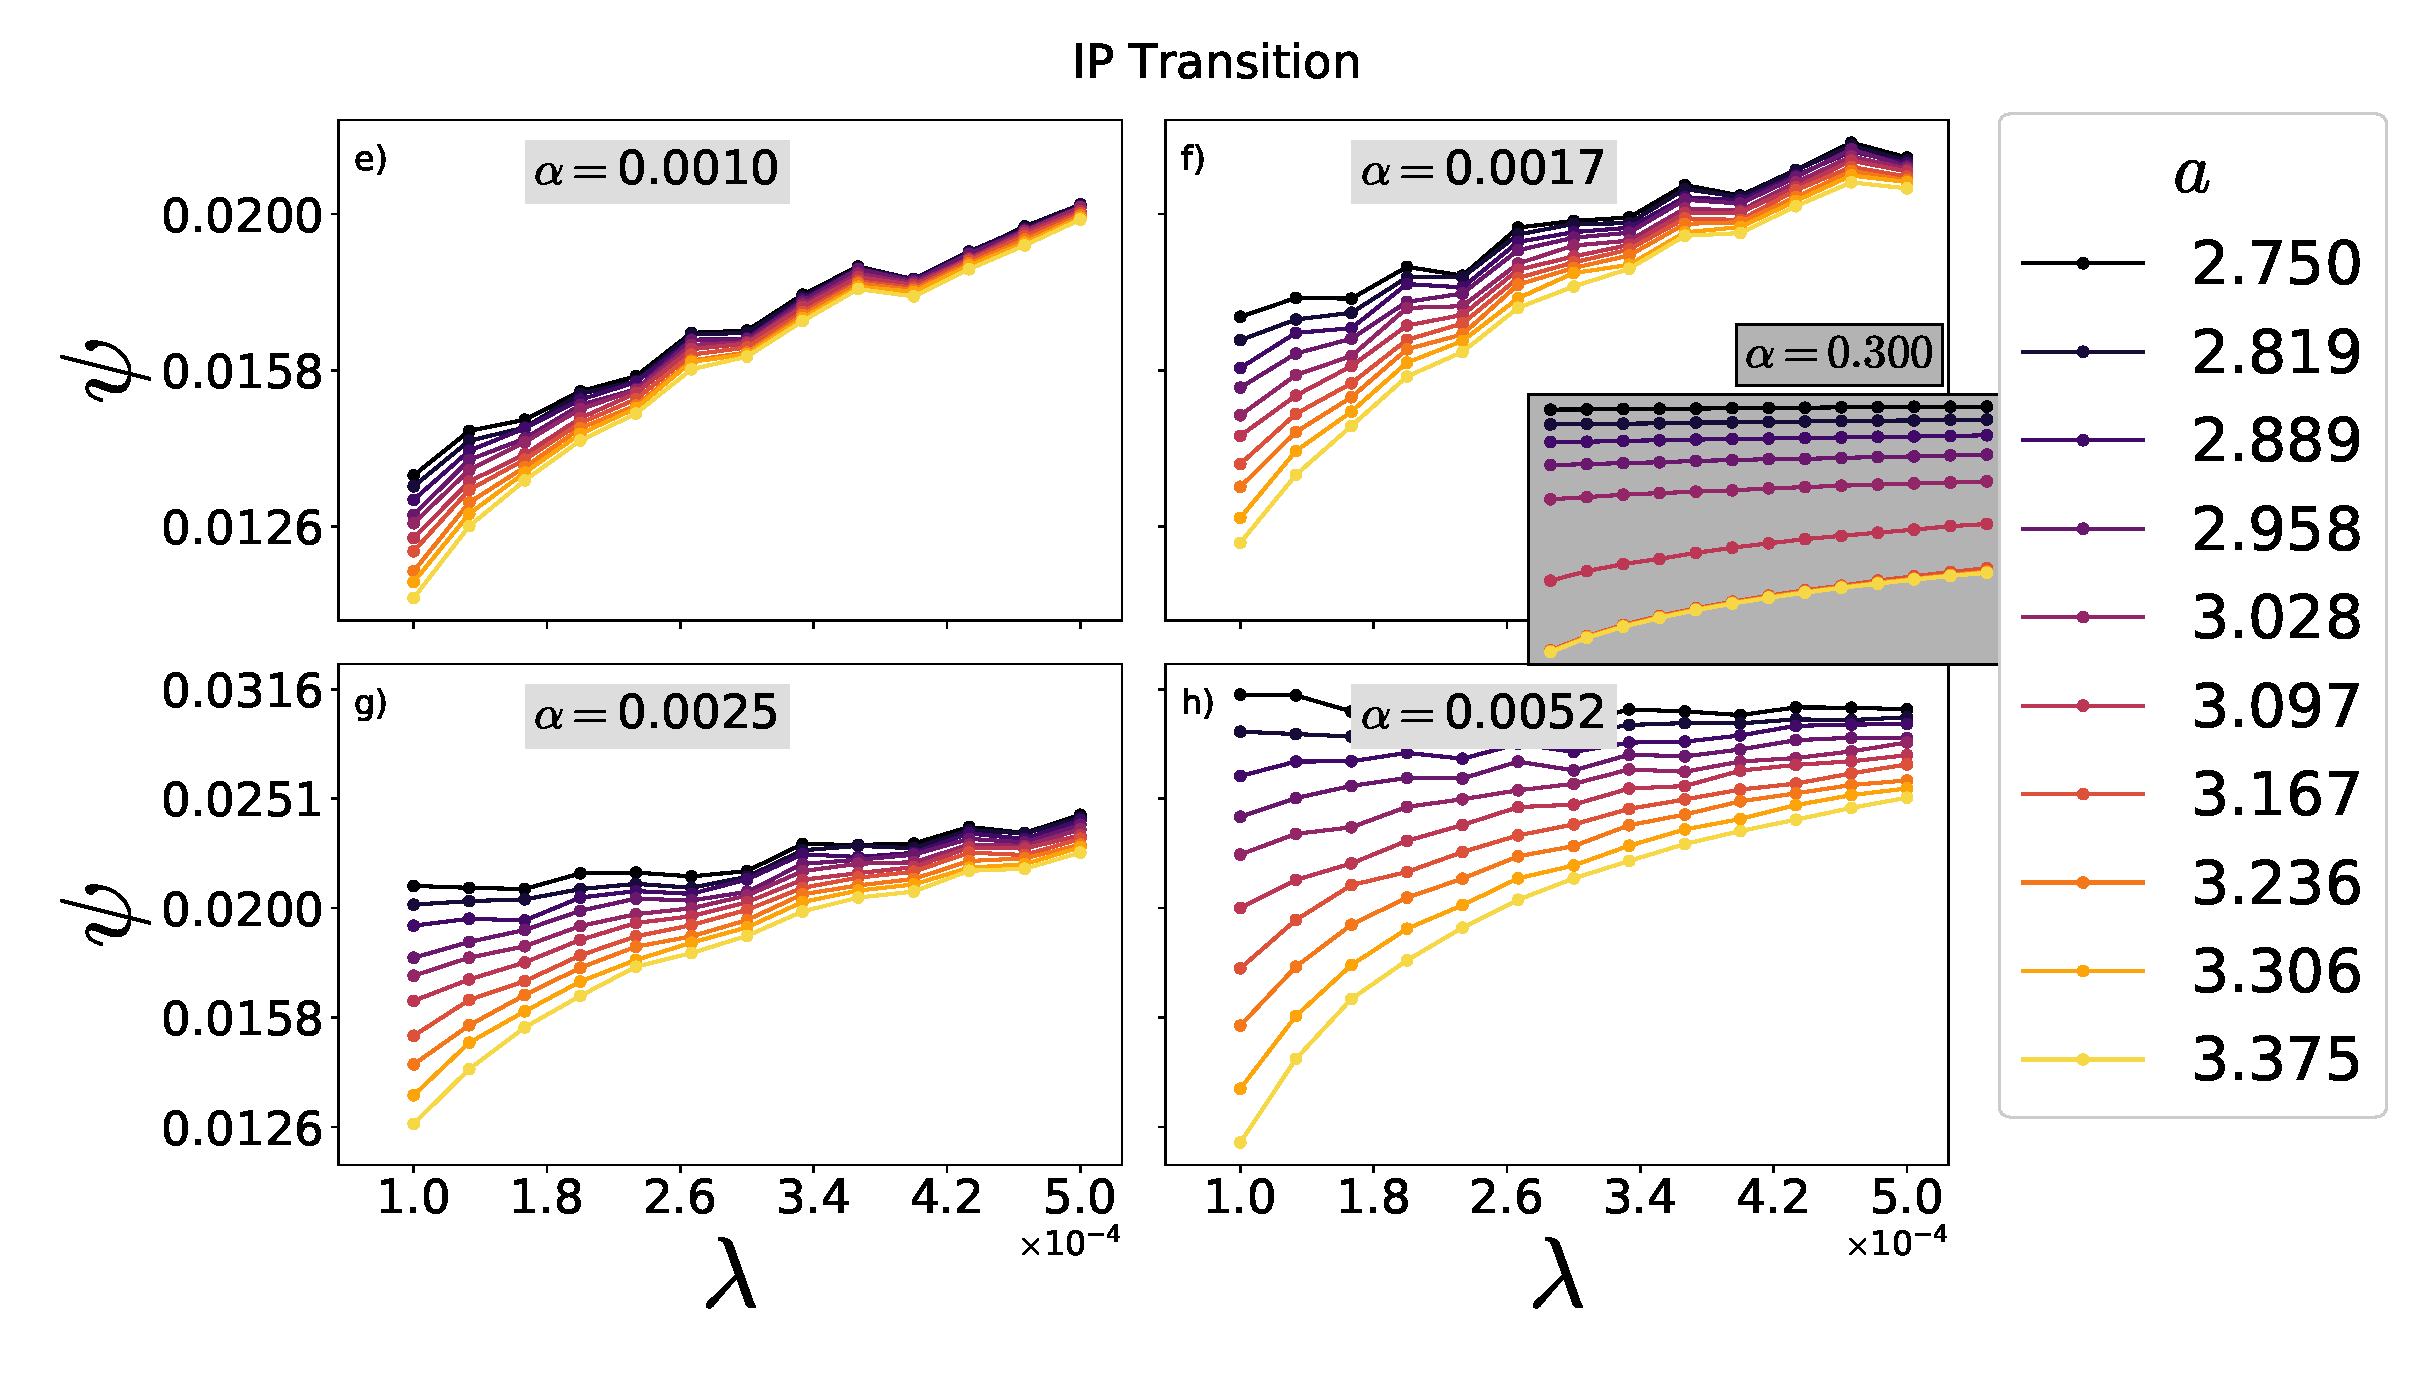
\includegraphics[width=0.85\linewidth]{fig/opsplit-psi-ipt.eps}
\end{center}
\caption{\label{fig:opsplit} (Color online) Order parameter $\psi$ versus inverse system size $\lambda$ for various values of $\alpha$,
    and coupling strengths $a$ in the vicinity of the GO and IP phase transitions. The insets in \textbf{b} and \textbf{f} show the
    behavior for $\alpha=0.3$, approaching the complete graph, with GO and IP transitions near $a_c=1.5$ and $a^c\approx3.1$
    respectively.  Each point represents an average over 400 independent realizations.  The oscillatory behavior seen in some panels is
due to the reduction in average path lengths caused by the introduction of new neighbors as the system size increases at fixed
$\alpha$, and the fact that $K$ must be an integer (see Appendix \ref{appendix:LC}).}
\end{figure}

In this context it is useful to plot the order parameter versus $\lambda\equiv1/N$. An upward (downward) curvature as $\lambda \to 0$
signals a nonzero (zero) value of the order parameter. In Fig.~\ref{fig:opsplit}, such plots are shown for selected values of $\alpha$
\footnote{{See full animations of Fig.~\ref{fig:opsplit}:
\href{https://youtu.be/pPQbc0eiv_4}{GO transition}},
\href{https://youtu.be/_qfNzoBpRO4}{IP transition}}
and system sizes up to $N=10^4$.  In panel b) we see evidence of the GO transition for the value $\alpha=0.0017$ in the form of an
inversion in curvatures for lines of constant coupling strength, which happens at $a_c \approx 2$.  The inset in this same panel shows
that for large $\alpha$ there is a clear split near the complete graph value $a_c=1.5$.  In the case of the IP transition we observe
that there is no upward curvature at any point, but rather a sharp increase in density of the lines of constant $a$ for higher values
of $\alpha$, as seen in the bottom inset of Fig.~\ref{fig:opsplit} where the lines $a=3.375$ and $a=3.306$ have collapsed to the same
point near the origin.

\begin{figure}
\begin{center}
    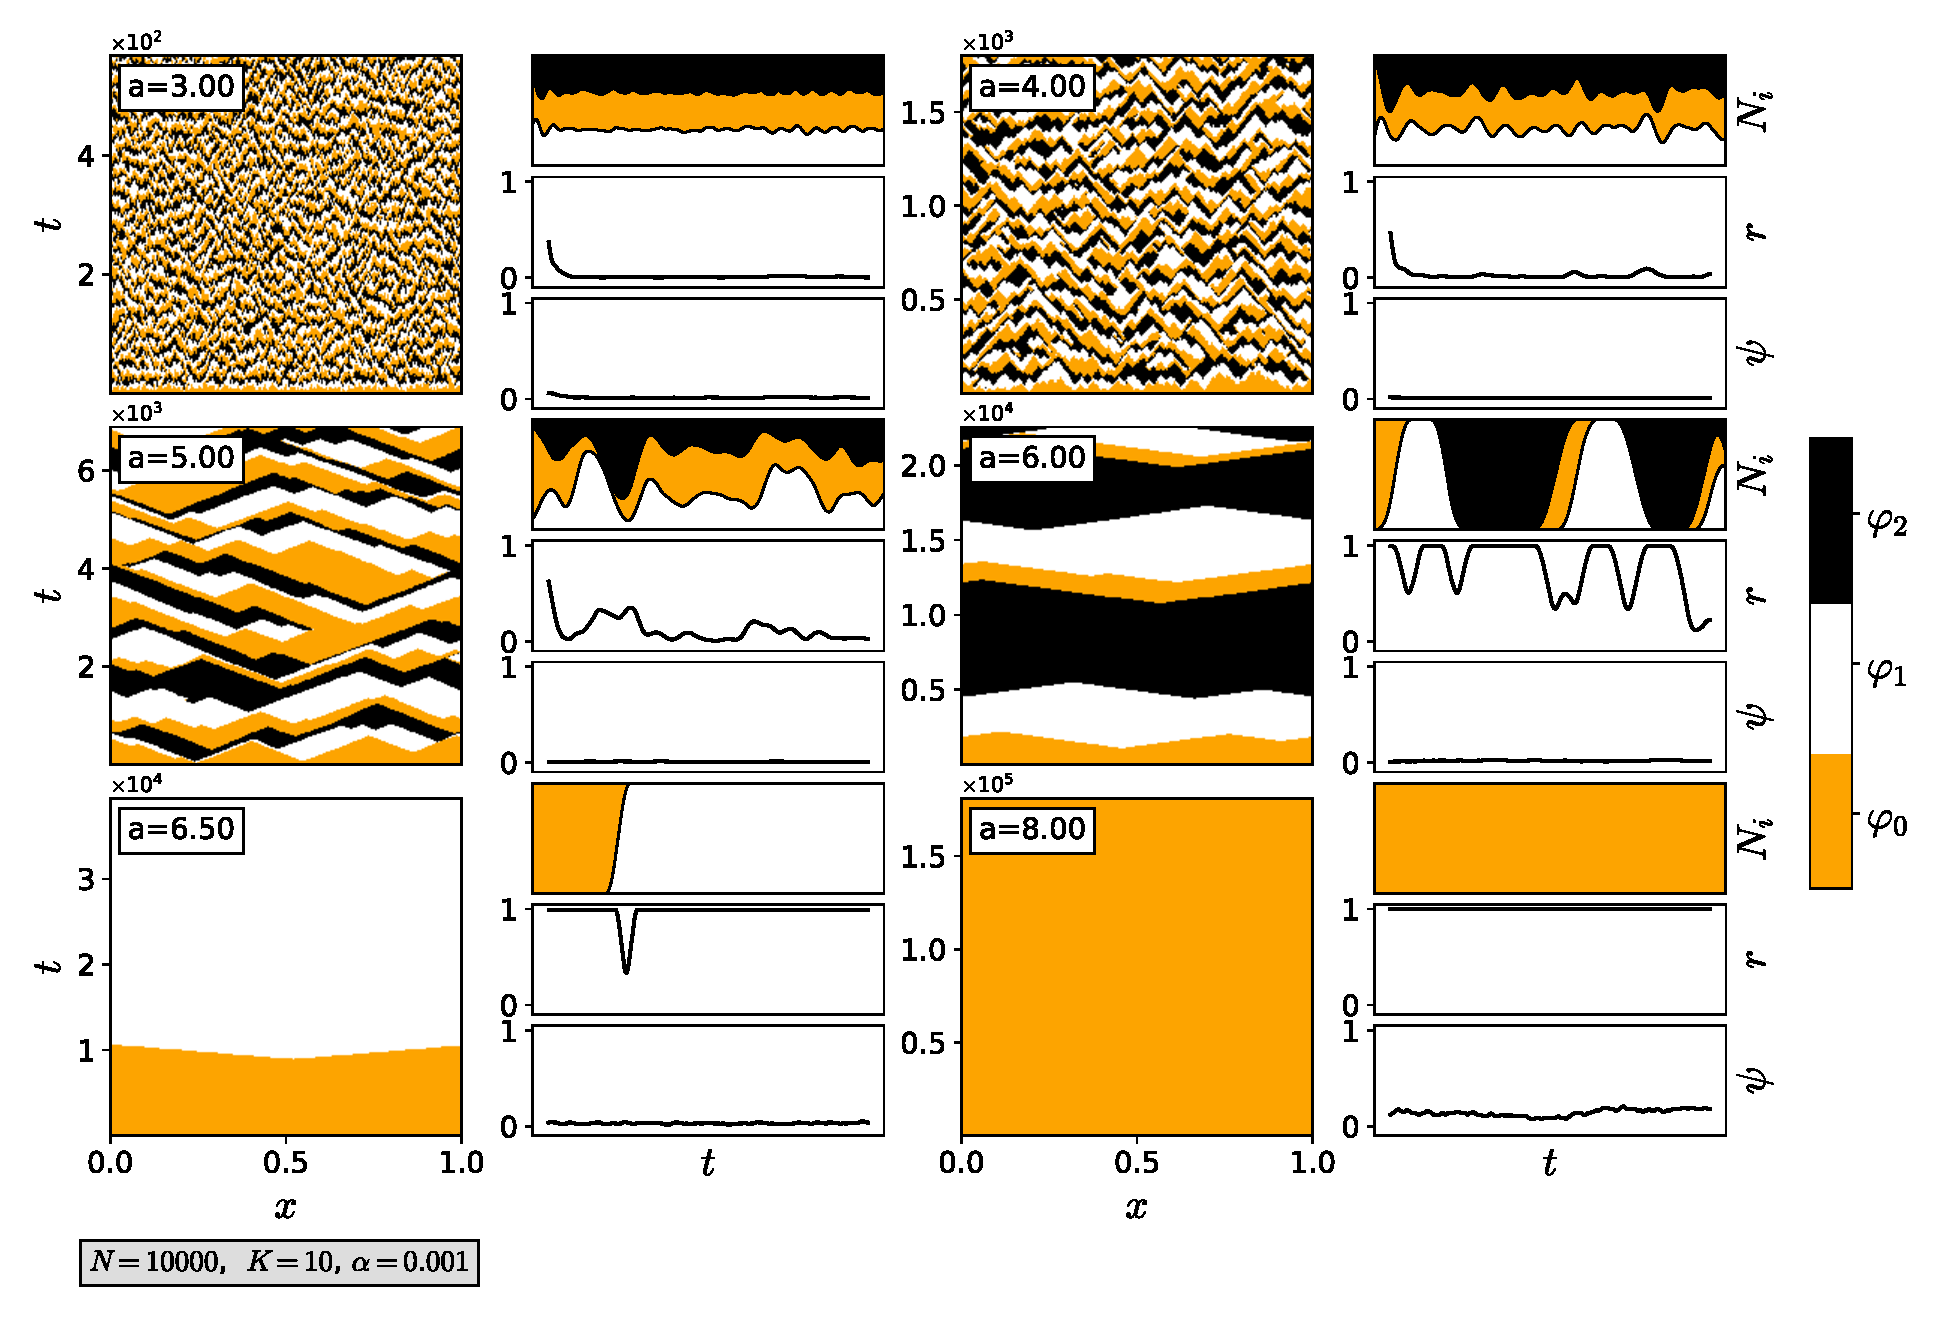
\includegraphics[width=1.\textwidth]{fig/articuno_figure_panel.eps}
\caption{\label{fig:trialpanel} Space-time plots, populations $N_i$, $\psi$ and $r$ order parameters. In all panels $N=10^4$, $K=10$
    and $\alpha=10^{-3}$. The images on the left and center-right columns show space-time plots with position on the horizontal axis
    and time increasing upward.  Adjacent and to the right of each space-time plot, three graphs show the corresponding populations,
    $\psi$, and $r$ as functions of time.  Here we see that for a large system with low connectivity there are no regular oscillations.
Instead, there are wave fronts that propagate and interfere and whose periods and amplitudes grow with $a$.  }
\end{center}
\end{figure}

Inspecting individual realizations of the dynamics in the small-$\alpha$ regime (Fig.~\ref{fig:trialpanel}) we see that the system
never shows global synchronization. It instead exhibits wave-like patterns that propagate in both directions, similar to what is
observed for large negative coupling~\cite{escaff2014arrays}, but here for $a$ positive . The amplitude and period of the wave increase
with $a$ and with system size (for fixed $\alpha$), which suggests there is an IP phase in the limit $N\to\infty$.

\subsection{Initial configuration dependence}

\begin{figure}[b]
\begin{center}
    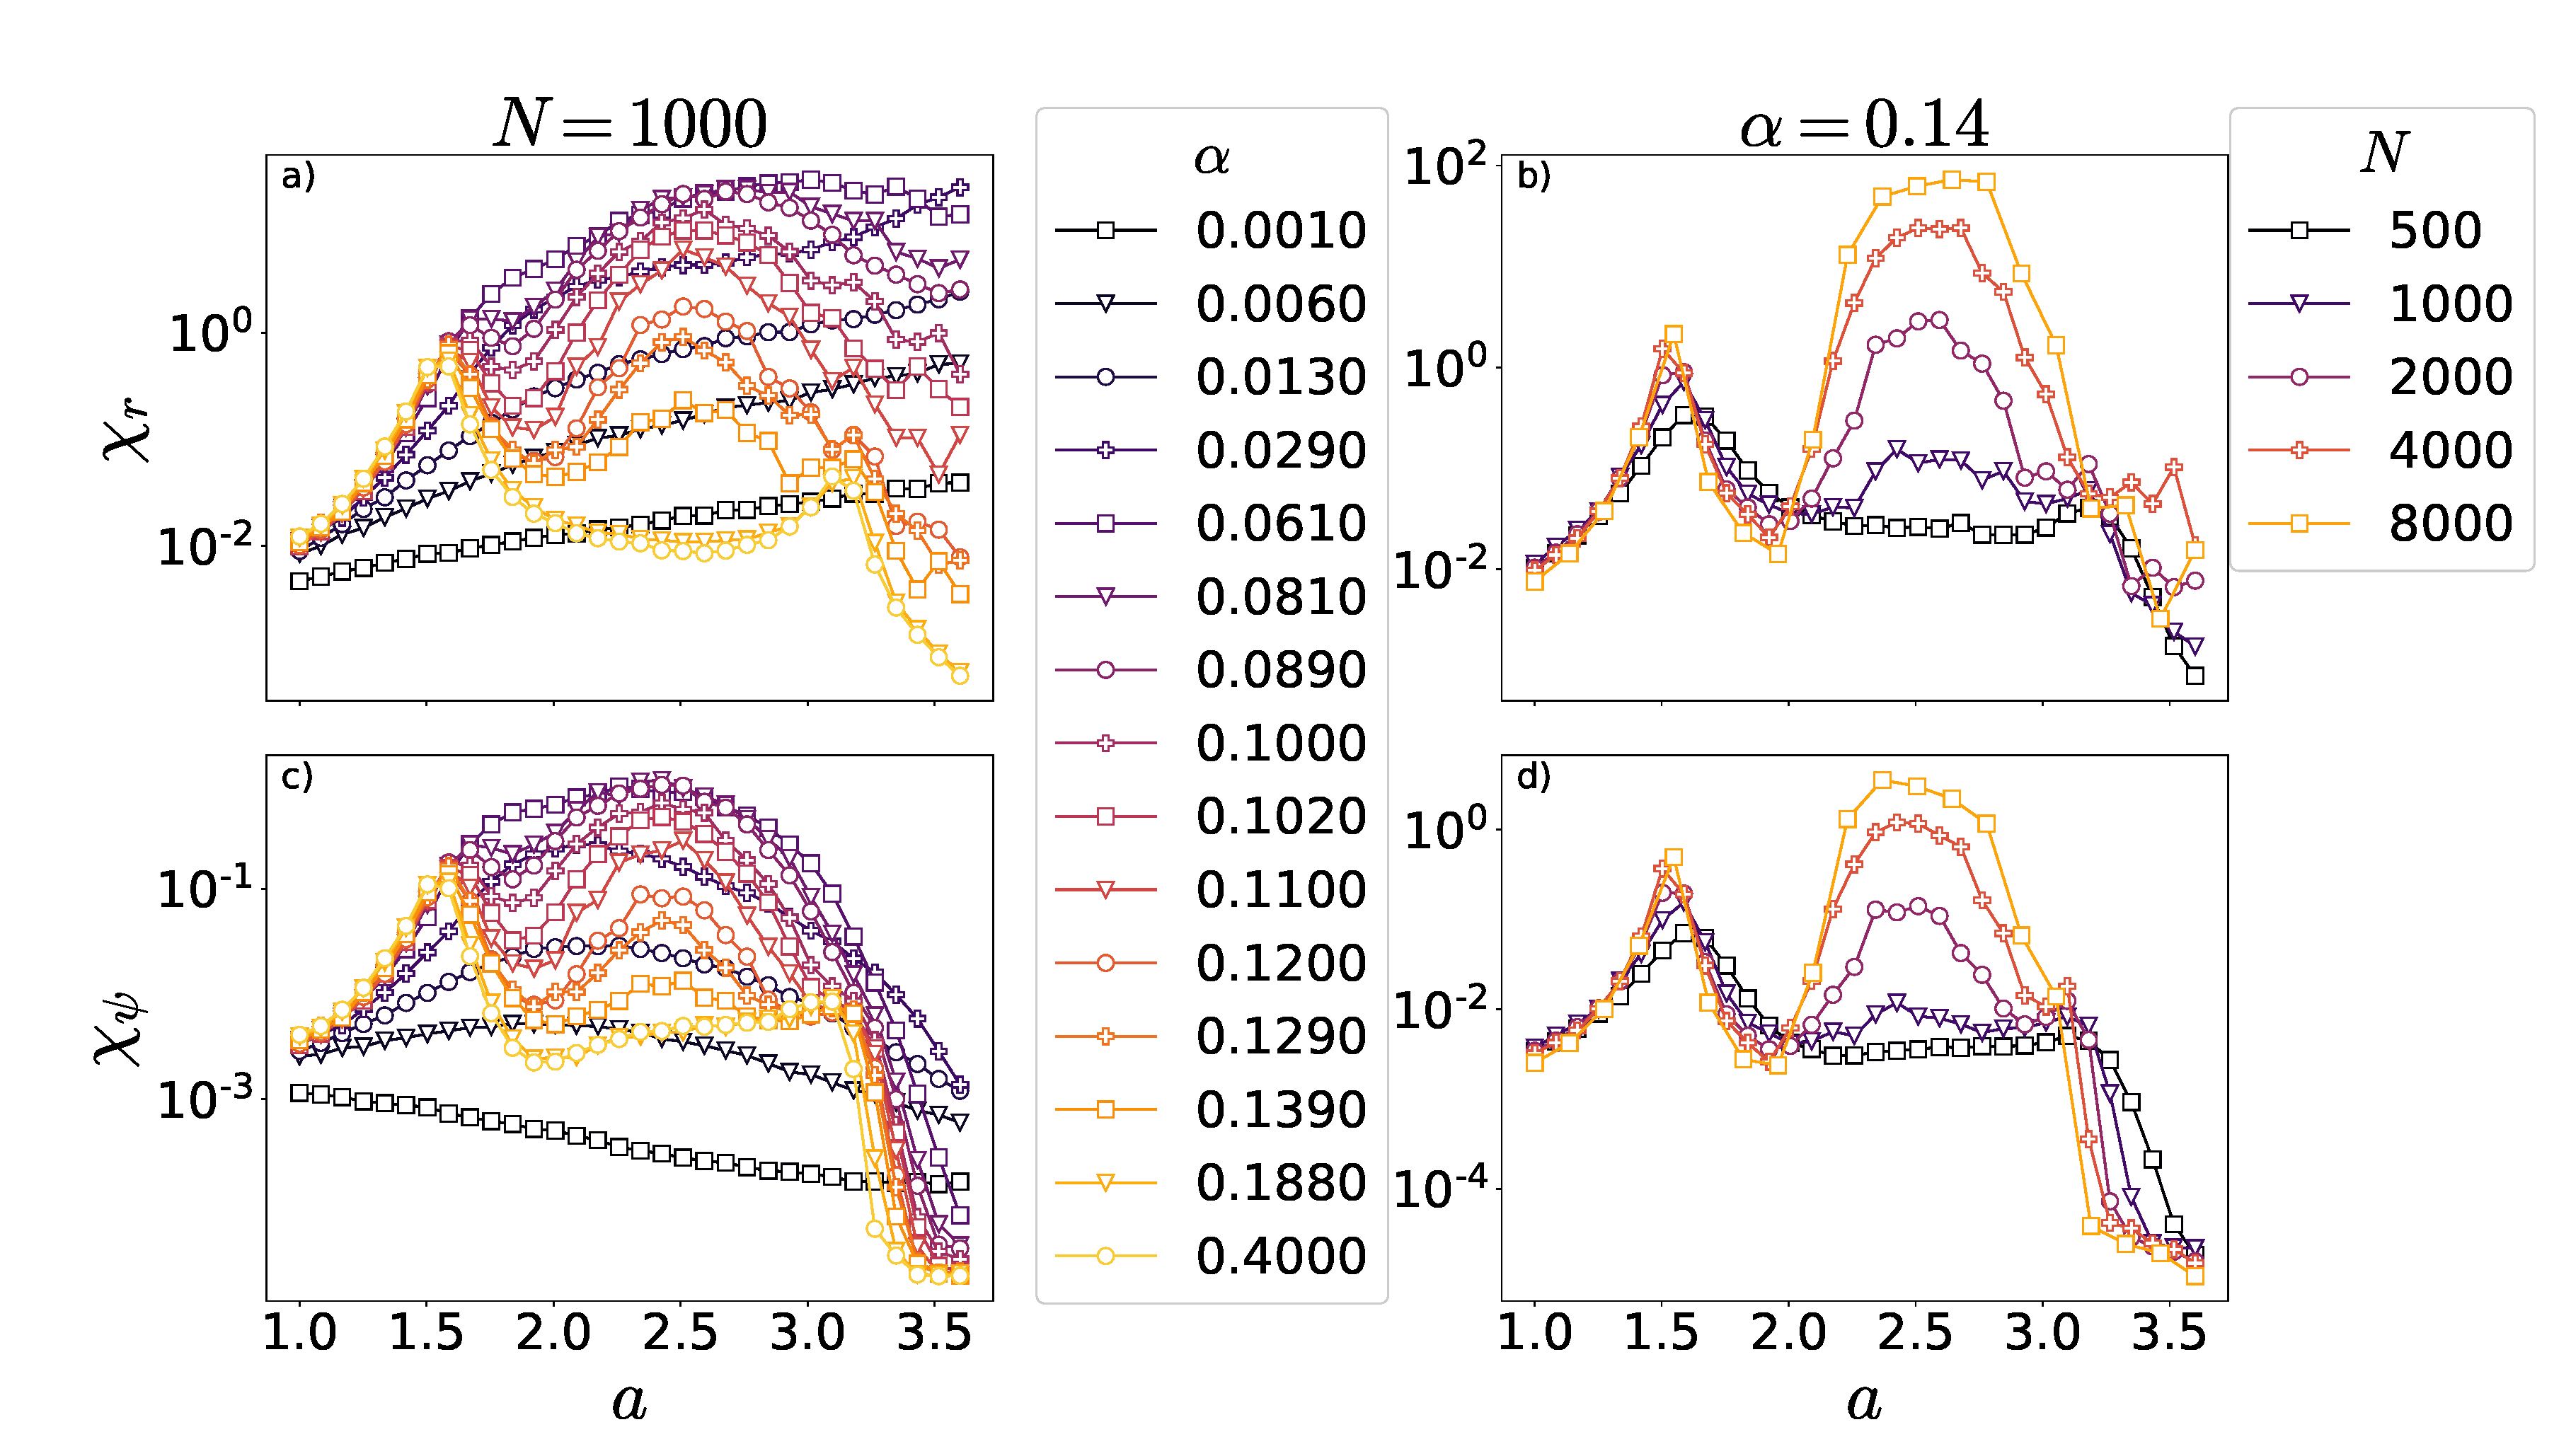
\includegraphics[width=0.95\textwidth]{fig/chi_curves_randomic.eps}
\caption{\label{fig:chicurvesrandom} (Color online) Scaled variances $\chi_r$ and $\chi_{\psi}$ for random initial conditions.  Left
column: fixed system size $N=1000$ with increasing $\alpha$.  Right column: fixed $\alpha=0.14$ and increasing system sizes.  Points
represent an average over 4000 independent realizations with random initial configurations.}
\end{center}
\end{figure}

Up to this point, all the results discussed were obtained using uniform initial configurations (ICs).  In
Fig.~\ref{fig:chicurvesrandom} shows $\chi_r$ and $\chi_{\psi}$ for \textit{random} ICs. The striking difference, compared to the results
for uniform ICs, is the presence of a middle peak between the two identified previously. The scaling behaviors (panels \textbf{b} and
\textbf{d}) suggest that the effect persists for large system sizes if $\alpha$ is held constant. High values of $\chi$ result from
multiple realizations of the dynamics that produce net averages of the order parameter that differ from one to another. At the
(continuous) GO and IP phase transitions, the values of the order parameter fluctuate strongly, giving rise to the peaks at $a=1.5$ and
$a\approx 3.1$. Another situation which may lead to high $\chi$ values is a bi-stability between configurations that have large values
of the order parameter and others having a small one, even when fluctuations associated with each configuration are small. This
suggests a \textit{discontinuous} phase transition where for some values of $\alpha$ the system can relax to multiple steady states. 

Space-time plots of the dynamics with coupling $a\approx 2.5$ and $\alpha=0.14$ reveal that this is indeed the case
(Fig.~\ref{fig:trialpanel2}).  Three examples are shown in Fig.~\ref{fig:trialpanel2}: on the left is the familiar globally
synchronized state, while the middle panel shows a travelling-wave state similar to those observed in \cite{escaff2014arrays}, (but
here, for large, positive coupling). The existence of a steady state with zero order parameter but $a>a_c$ is surprising since
Fig.~\ref{fig:chicurvesrandom} suggests that wave-like solutions persist even in the limit $N\to\infty$ (with fixed $\alpha$), where
interaction ranges become infinite.

\begin{figure}
\begin{center}
    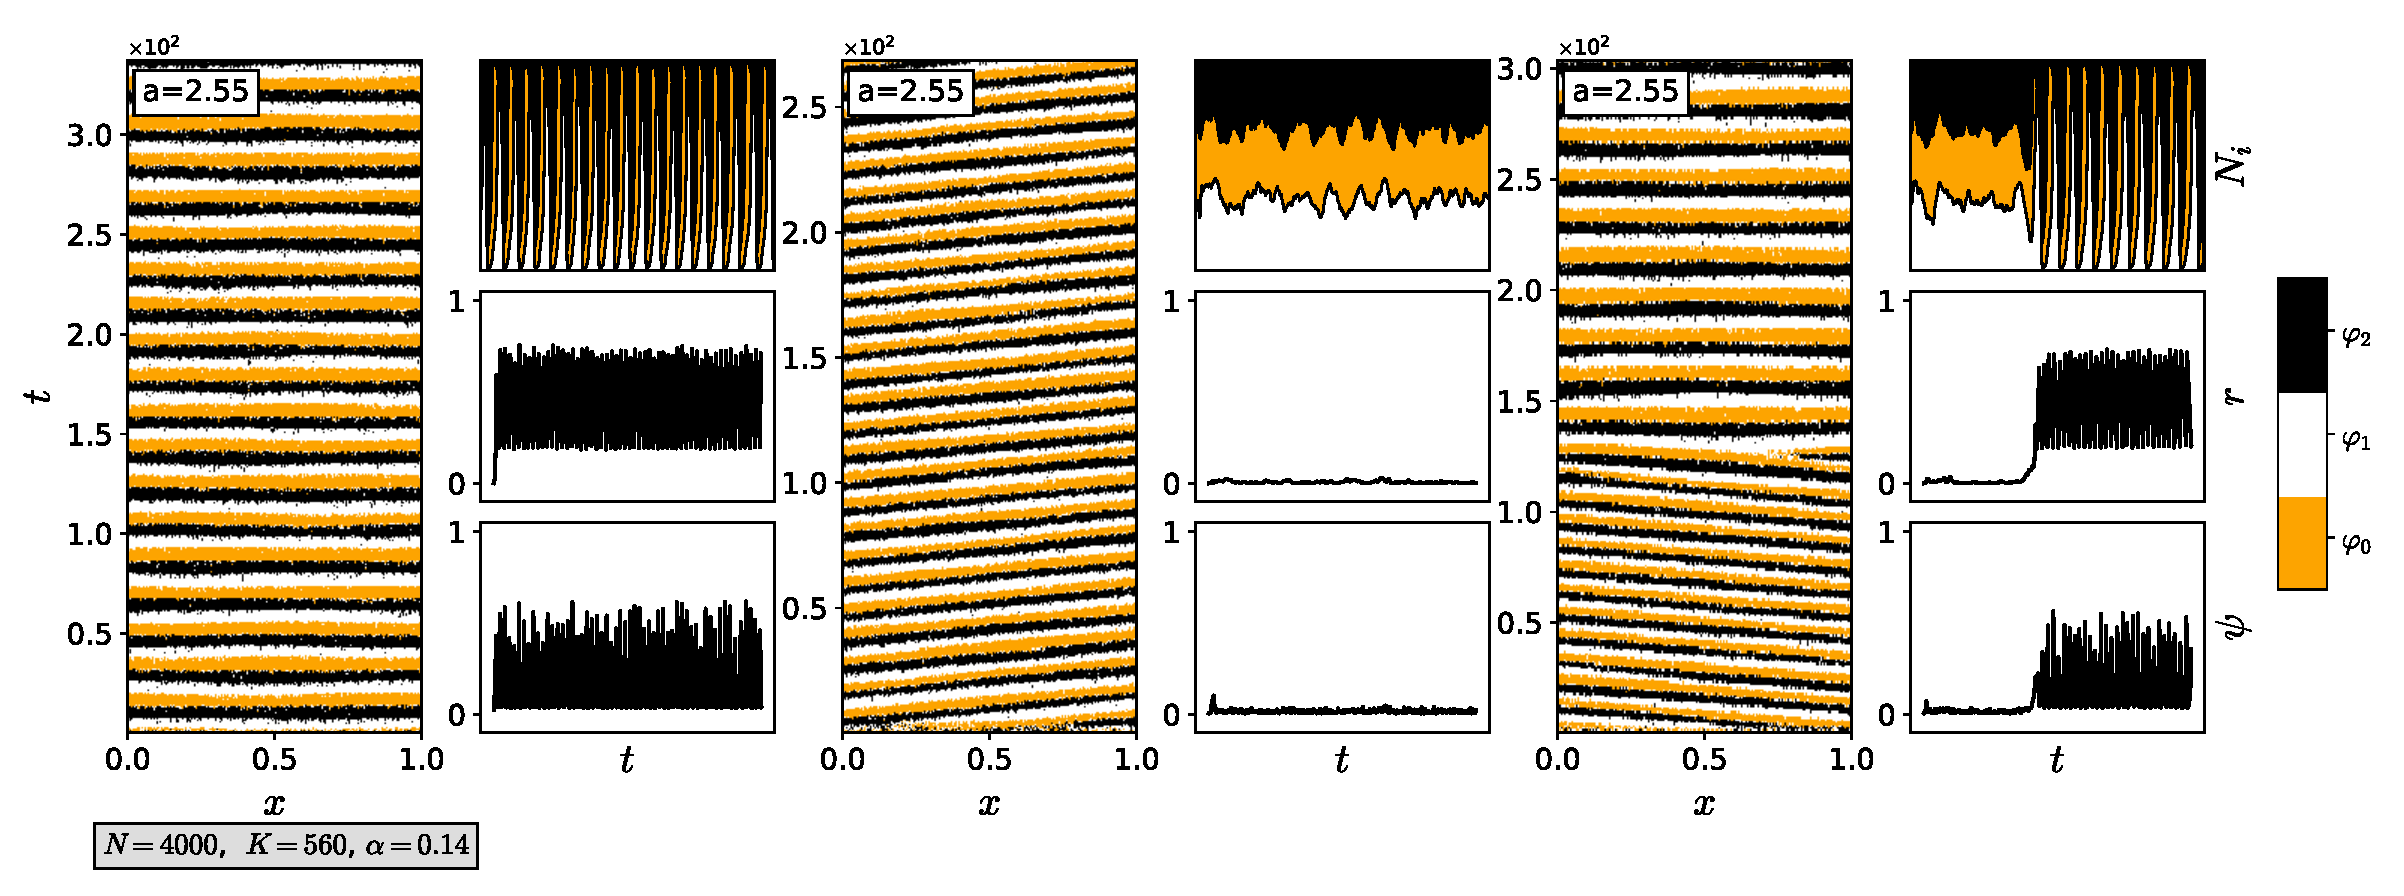
\includegraphics[width=1.\textwidth]{fig/articuno_figure_panel2.eps}
\caption{\label{fig:trialpanel2} Single realizations with random initial configurations. Left: Global oscillations. Middle: travelling
wave. Right: fluctuation-induced change from a travelling wave to global oscillations.  The fraction of realizations that converge to
travelling waves is approximately $1.6\%$. In all panels $N=4000$, $K=560$, $a=2.55$.}
\end{center}
\end{figure}

The rightmost panel in Fig.~\ref{fig:trialpanel2} shows a fluctuation-induced change from a travelling wave to global synchrony.  Such
transitions allow the average order parameter to attain values between those associated with a wave state and a globally synchronized
one, being closer to one or the other depending on what fraction of time it spent at that particular configuration.  Starting from
\textit{random} ICs, about 1.6\% of realizations exhibit travelling waves, but since $\psi\approx 0$ for the waves and $\psi \sim
\mathcal{O}(1)$ for the globally synchronized case, the variances $\chi_r$ and $\chi_{\psi}$ are sensitive even to small rates of
occurrence.  Due to fluctuations, waves do not persist in smaller systems; sizes $N \geq 700$ are required. Smaller systems exhibit
either disordered phases with domains that increase in size and duration as the coupling grows, or global synchrony if the interaction
range $K$ is large enough.  In all cases, waves with exactly one spatial period over the system are observed, while for negative
coupling, multiple stable wave numbers are found depending on the coupling magnitude \cite{escaff2014arrays}.

\begin{figure}[b]
\begin{center}
    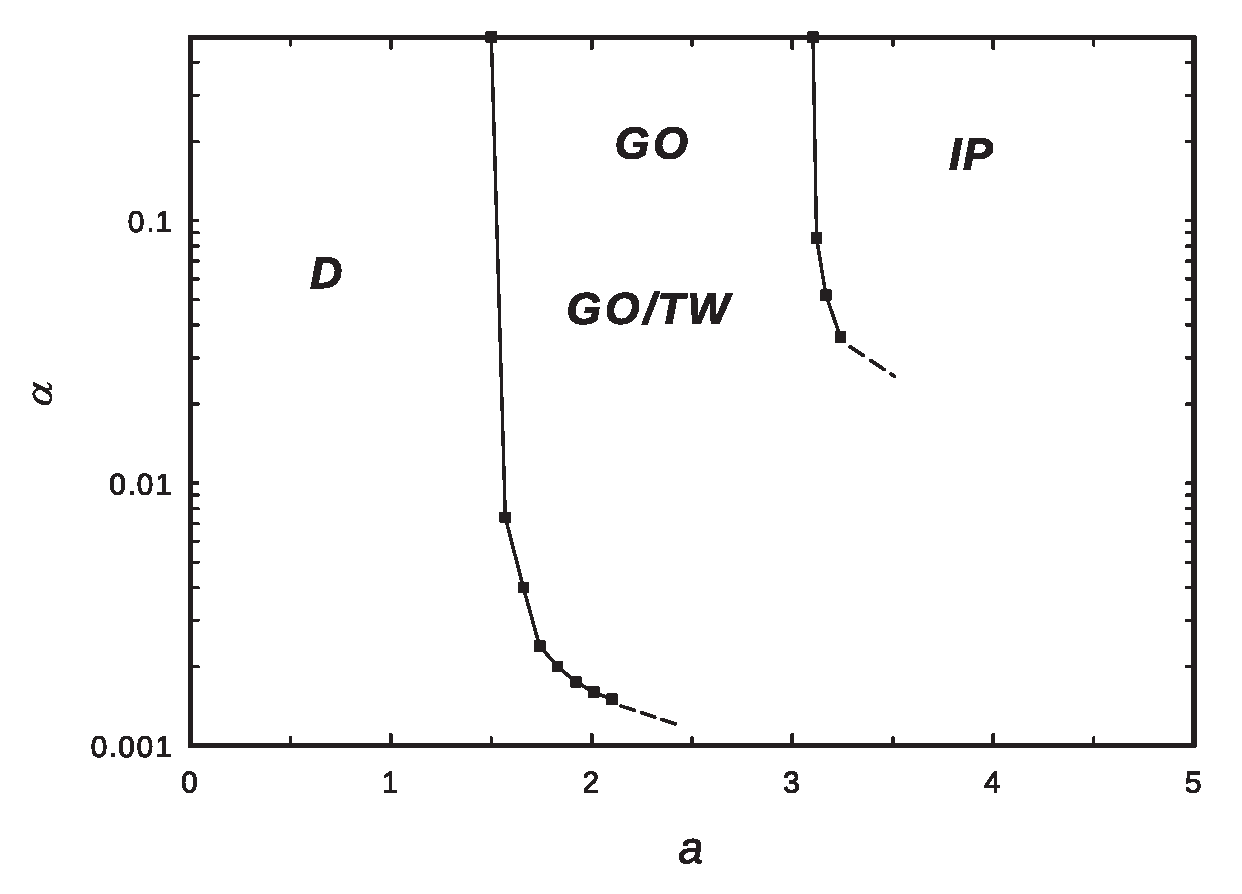
\includegraphics[width=1.\textwidth]{fig/phasediag.eps}
\caption{\label{fig:phase_diagram} Regular rings: Preliminary phase diagram in the $a$-$\alpha$ plane.  Points are simulation results
and (for $\alpha=0.5$) exact values.  Lines are guides to the eye.  Dashed lines represent our conjectures for how the phase boundaries
continue.  Phases: disordered (D); global oscillation (GO); travelling-wave (TW); infinite- period (IP).}
\end{center}
\end{figure}

The existence of travelling waves can be understood by noting that, for $\alpha<0.5$, the system consists of $G=N/2K$ domains. $G$
represents the average path length for regular rings. (See Appendix~\ref{appendix:LC}.) When $G$ is a multiple of three, the system is
capable of containing a full wavelength without oscillators in the center of the domains. The wavefronts are then able to propagate as
nucleation fronts \cite{assis2011infinite} giving rise to travelling waves. In our simulations, with $N \leq10^4$, we find only one
stable wave-number (a wave with period $N$). This is in contrast with the wave patterns observed in \cite{escaff2014arrays}, where
multiple wave-numbers were identified as stable depending on the magnitude of the coupling strength.

Although travelling waves are rare starting from random ICs, initializing with solid blocks of 0s, 1s and 2s, each occupying one third
of the system, the ensuing evolution consists of a stable travelling wave in nearly all cases.  Thus the rarity for random ICs simply
reflects the low probability of provoking a wave, and does not reflect an intrinsic instability of the travelling-wave state.  ICs with
smaller blocks, such that the system contains two or more waves, invariably yield, following a transient, a travelling wave whose
wavelength equals the system size.


With the known phase transition points for $\alpha=0.5$ and the data from Figs.~\ref{fig:chicurvesrandom} and \ref{fig:opsplit} (for $N
\leq 10^4$) we are able to sketch the phase diagram (Fig.~\ref{fig:phase_diagram}). While the phase boundaries are rather insensitive
to changes in the connectivity for relatively large $\alpha$ values, they veer to larger couplings for small $\alpha$.


\section{\label{smallworld} The WCM on small-world networks}


\begin{figure}[b]
    \centering
    \begin{minipage}[t]{0.33\textwidth}
        \centering
        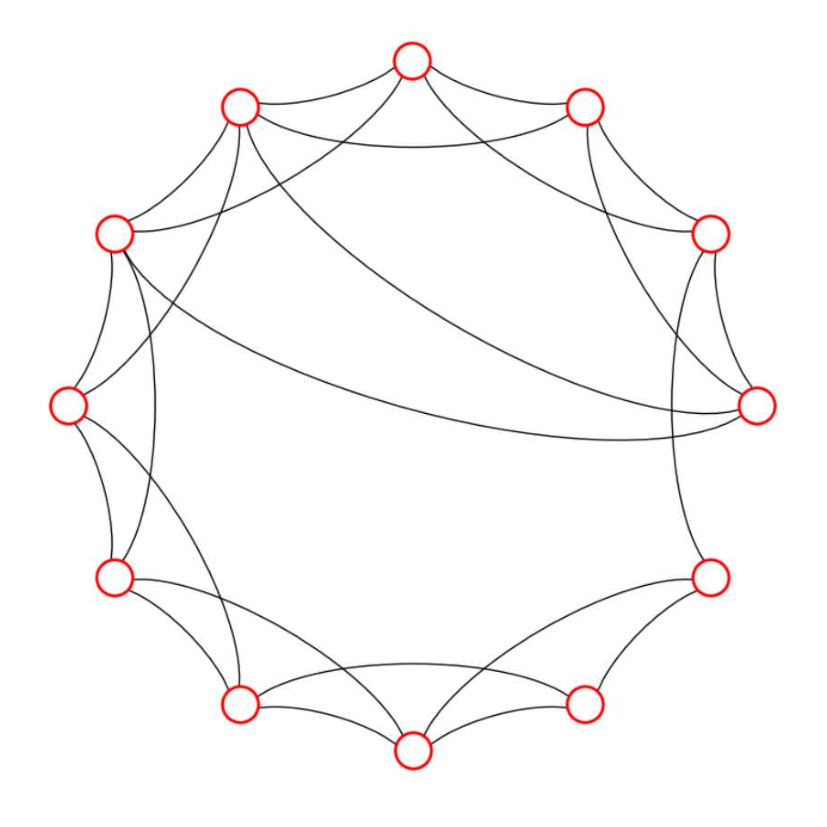
\includegraphics[width=0.9\textwidth]{fig/rewiredring.eps}
        \caption{\label{fig:rewiredring} Example of a rewired regular ring with $N=12$, $K=2$ and $p=0.1$.  }
    \end{minipage}
    \hfill
    \begin{minipage}[t]{0.62\textwidth}
        \centering
        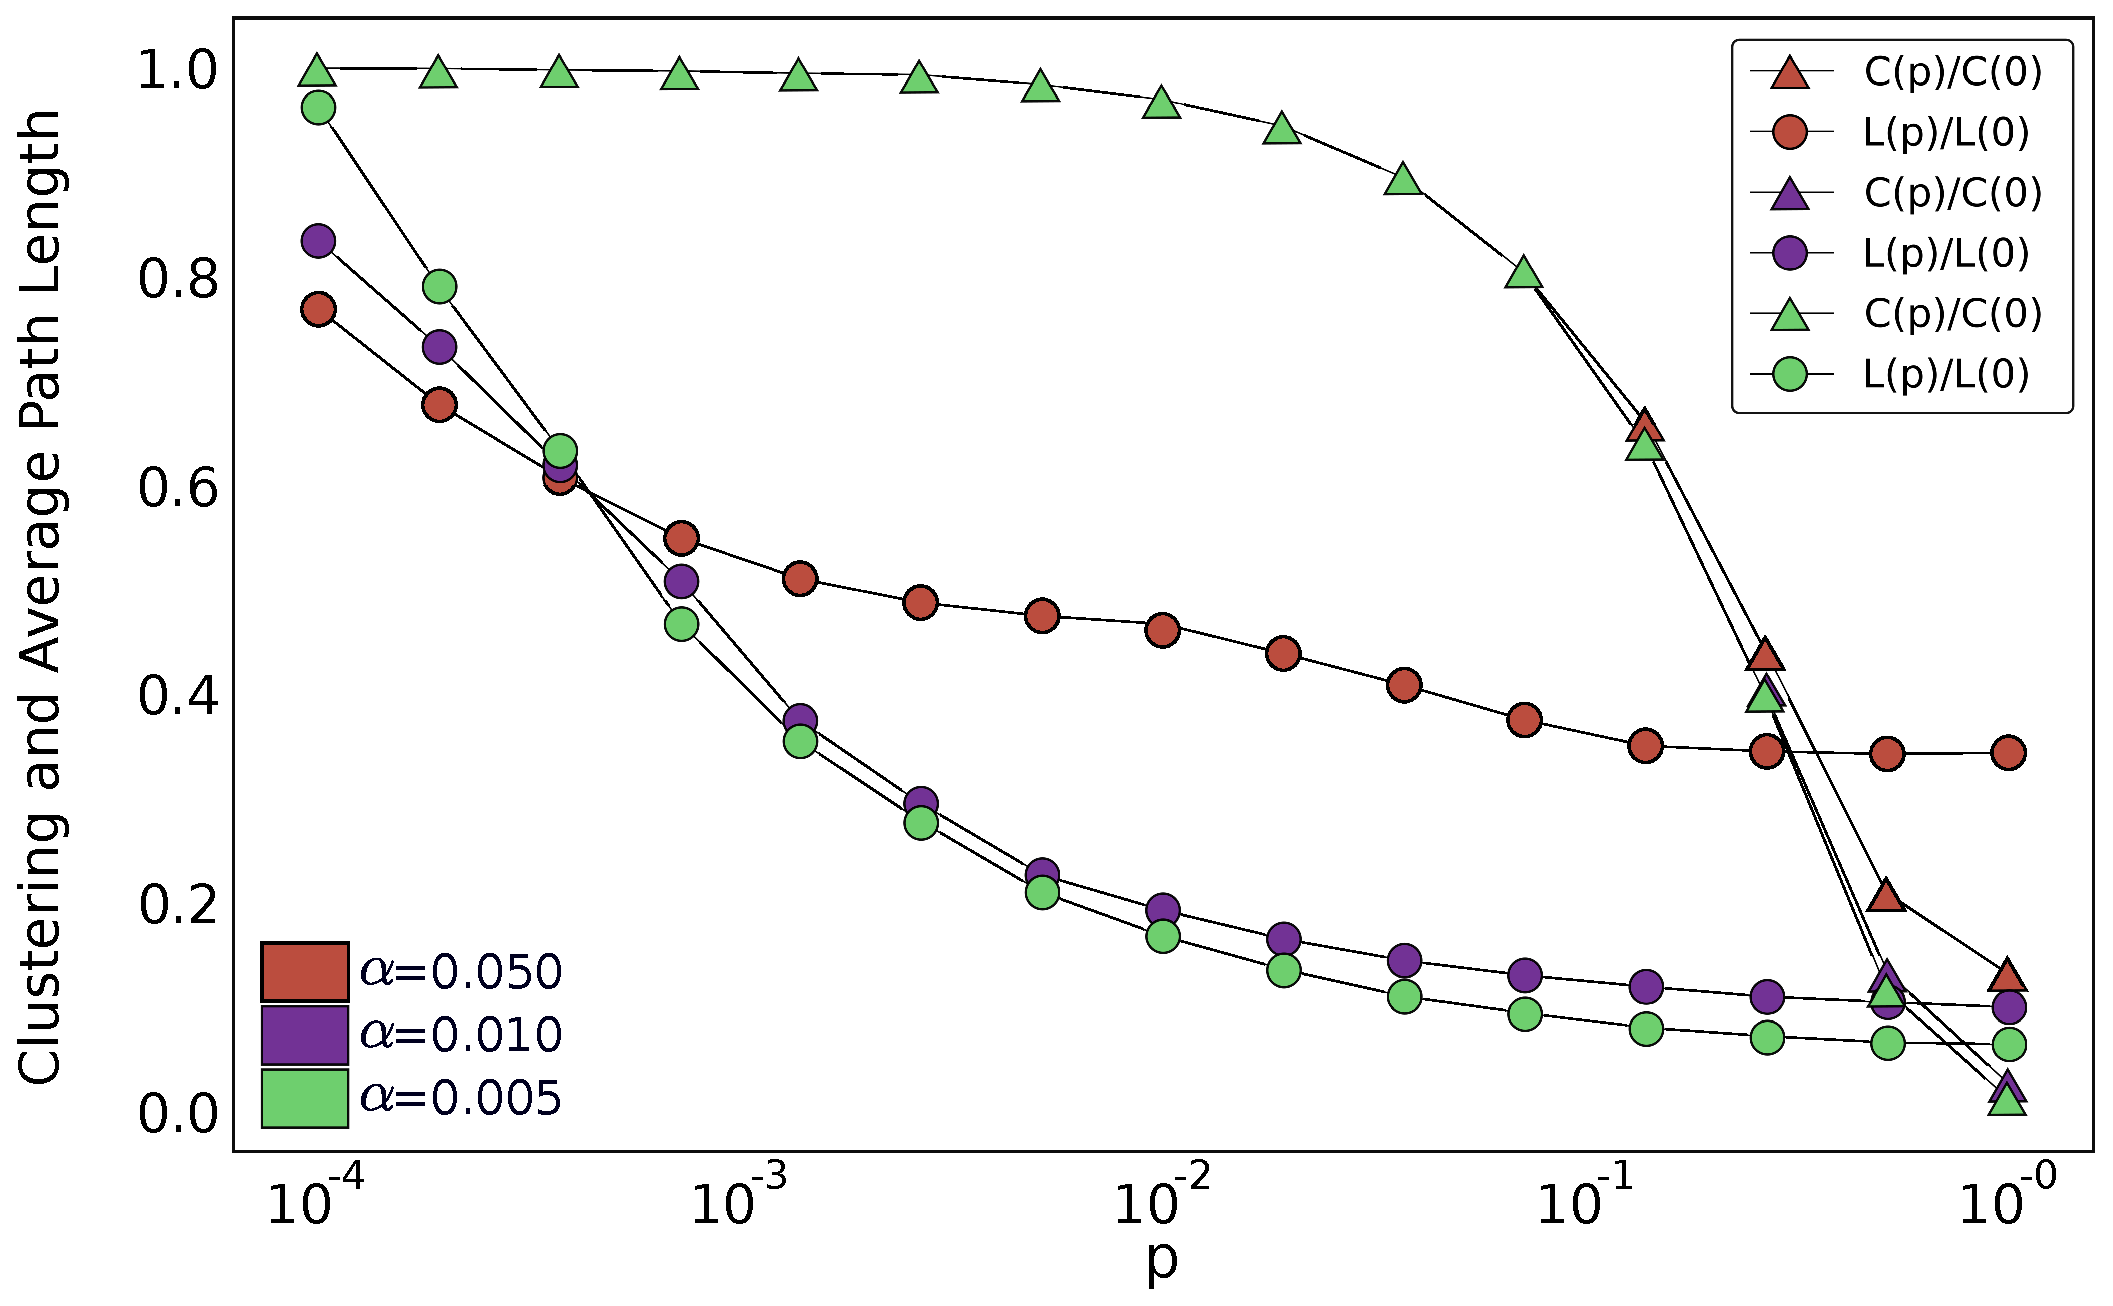
\includegraphics[width=0.9\textwidth]{fig/small-world.eps}
        \caption{\label{fig:small-world} (Color online) Clustering coefficient $C$ and mean path length $L$ versus rewiring probability
        $p$ for networks of $N=5000$ nodes.  $K=250, 50, 25$ for red, blue, green curves respectively. The data represent averages over
    400 independently generated networks.  }
    \end{minipage}
\end{figure}

Regular rings can be used as the starting point for constructing \textit{small-world networks}, which are characterized by a small degree
of separation between nodes while maintaining local regions tightly clustered. A well known algorithm for generating this type of
network from regular rings was introduced by Watts and Strogatz~\cite{watts1998collective}. Starting from a regular ring, for each edge
in the graph, the clockwise node of that edge is swapped with probability $p$ for another randomly selected node, forbidding
self-connections or repeated edges. Some care may be taken to avoid disconnected graphs as a result of this process, but this is
unlikely for most parameter triplets ($N$, $K$, $p$) considered here~\cite{watts1998collective}. An example of such a rewired ring is
shown in Fig.~\ref{fig:rewiredring}.

To characterize a network as small-world, we define two quantities:

\begin{itemize}
    \item \textit{Mean path length} $L$: For nodes $i$ and $j$ in network $\mathcal{G}$, let $L_{ij}$ be the number of edges in the
        shortest path connecting these nodes.  Then the average path length of $\mathcal{G}$ is $L=\left<L_{ij} \right>$, where the
        average is over all pairs $(i,j)$ with $i<j$.
    \item \textit{Clustering coefficient} $C$: If node $i$ has $n_i$ neighbors, then the maximum possible number of connections among
        its neighbors is $m_i=\frac{n_i(n_i-1)}{2}$. Let $m^*_i$ be the number of connections among the neighbors of node $i$ in
        network $\mathcal{G}$. Then the clustering coefficient of $\mathcal{G}$ is $C=\left< \frac{m^*_i}{m_i} \right>$, where the average is
        over all nodes $i$.
\end{itemize}

Evidently, the maximum possible value for $C$ is $C=1$ and the minimum possible value for $L$ is $L=1$. For networks generated by
rewiring a regular ring graph, $C$ and $L$ are functions of the ring-graph parameters $N$ and $K$, as well as the rewiring probability
$p$: $L\equiv L(N,K,p)$, $C\equiv C(N,K,p)$. As shown in the Appendix, for regular rings (i.e., $p=0$), we have:

\begin{equation}
C(N,K,0)=
\begin{cases}
    0 ,                                      & \text{if } K<2 \\
    \frac{3K-3}{4K-2},                       & \text{if } 2 \leq K \leq
    \frac{N-1}{3} \\
    \frac{12K^2+6K-6KN+N^2-3N+2}{4K^2-2K},   & \text{if } \frac{N-1}{3} < K <
    \frac{N}{2} \\
    1,                                       & \text{otherwise}
\end{cases}
\end{equation}

\begin{equation}
L(N,K,0)=
\begin{cases}
    \frac{KG(G-1) + rG}{N-1}, & \text{if } K \leq \frac{N}{2} \\
    1,                        & \text{otherwise},
\end{cases}
\end{equation}

\noindent where $G$ is the largest integer smaller than $\frac{N-1}{2K}$ or,
using the floor operator,

\begin{equation*}
    G = \floor*{\frac{N-1}{2K}} .
\end{equation*}

For nonzero values of $p$ we generate graphs and take the averages for $C$ and $L$, as shown in Fig.~\ref{fig:small-world}. For
rewiring probabilities $p \in \left( 0.001, 0.1 \right)$, rewiring preserves the clustering property while greatly reducing the average
path length, thus characterizing small-world networks.

\begin{figure}
\begin{center}
    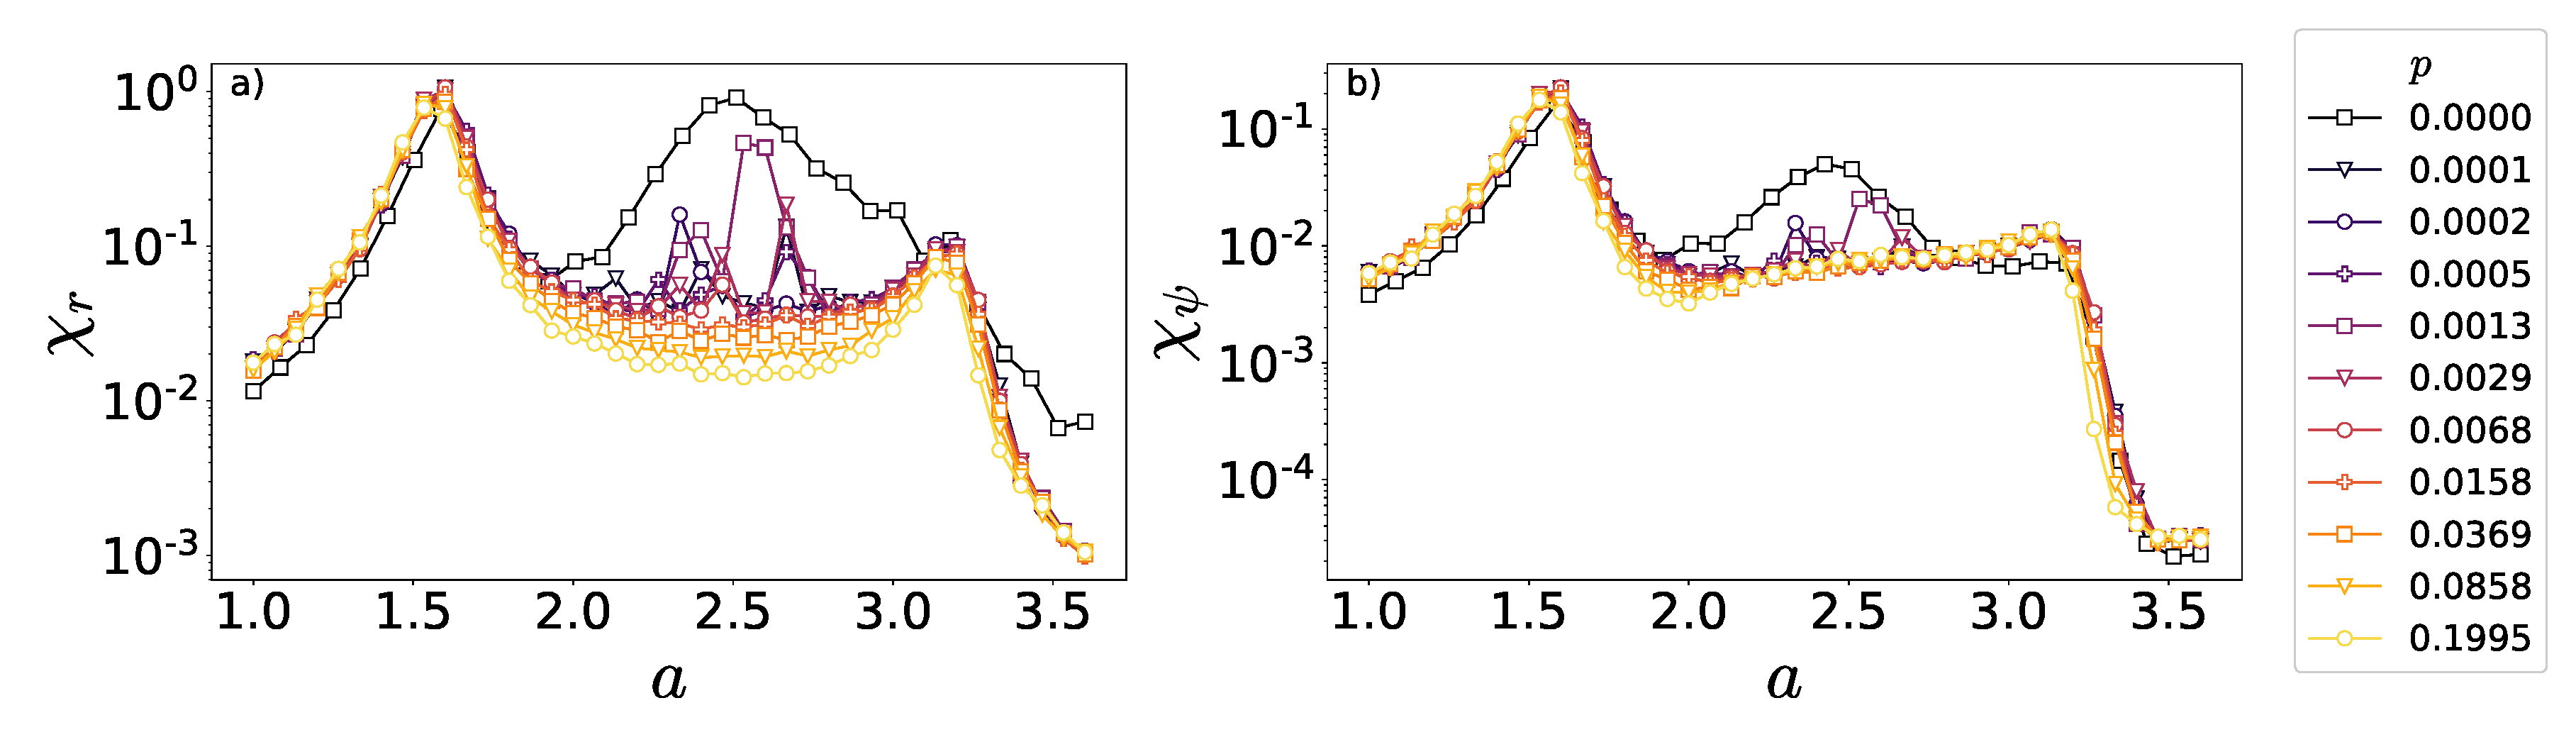
\includegraphics[width=1.\textwidth]{fig/chi_curves_pvalue.eps}
    \caption{\label{fig:chicurvespvalue} (Color online) Small-world networks: Scaled variances, $\chi_r$ and $\chi_{\psi}$, for
    increasing rewiring probabilities. $N=1000$, $K=129$, $\alpha=0.129$ with random initial conditions. For $p \approx 0.01$ the
curves follow their complete graph counterparts, even though the number of connections is half as many, and travelling waves become
unstable.  }
\end{center}
\end{figure}

\begin{figure}
\begin{center}
    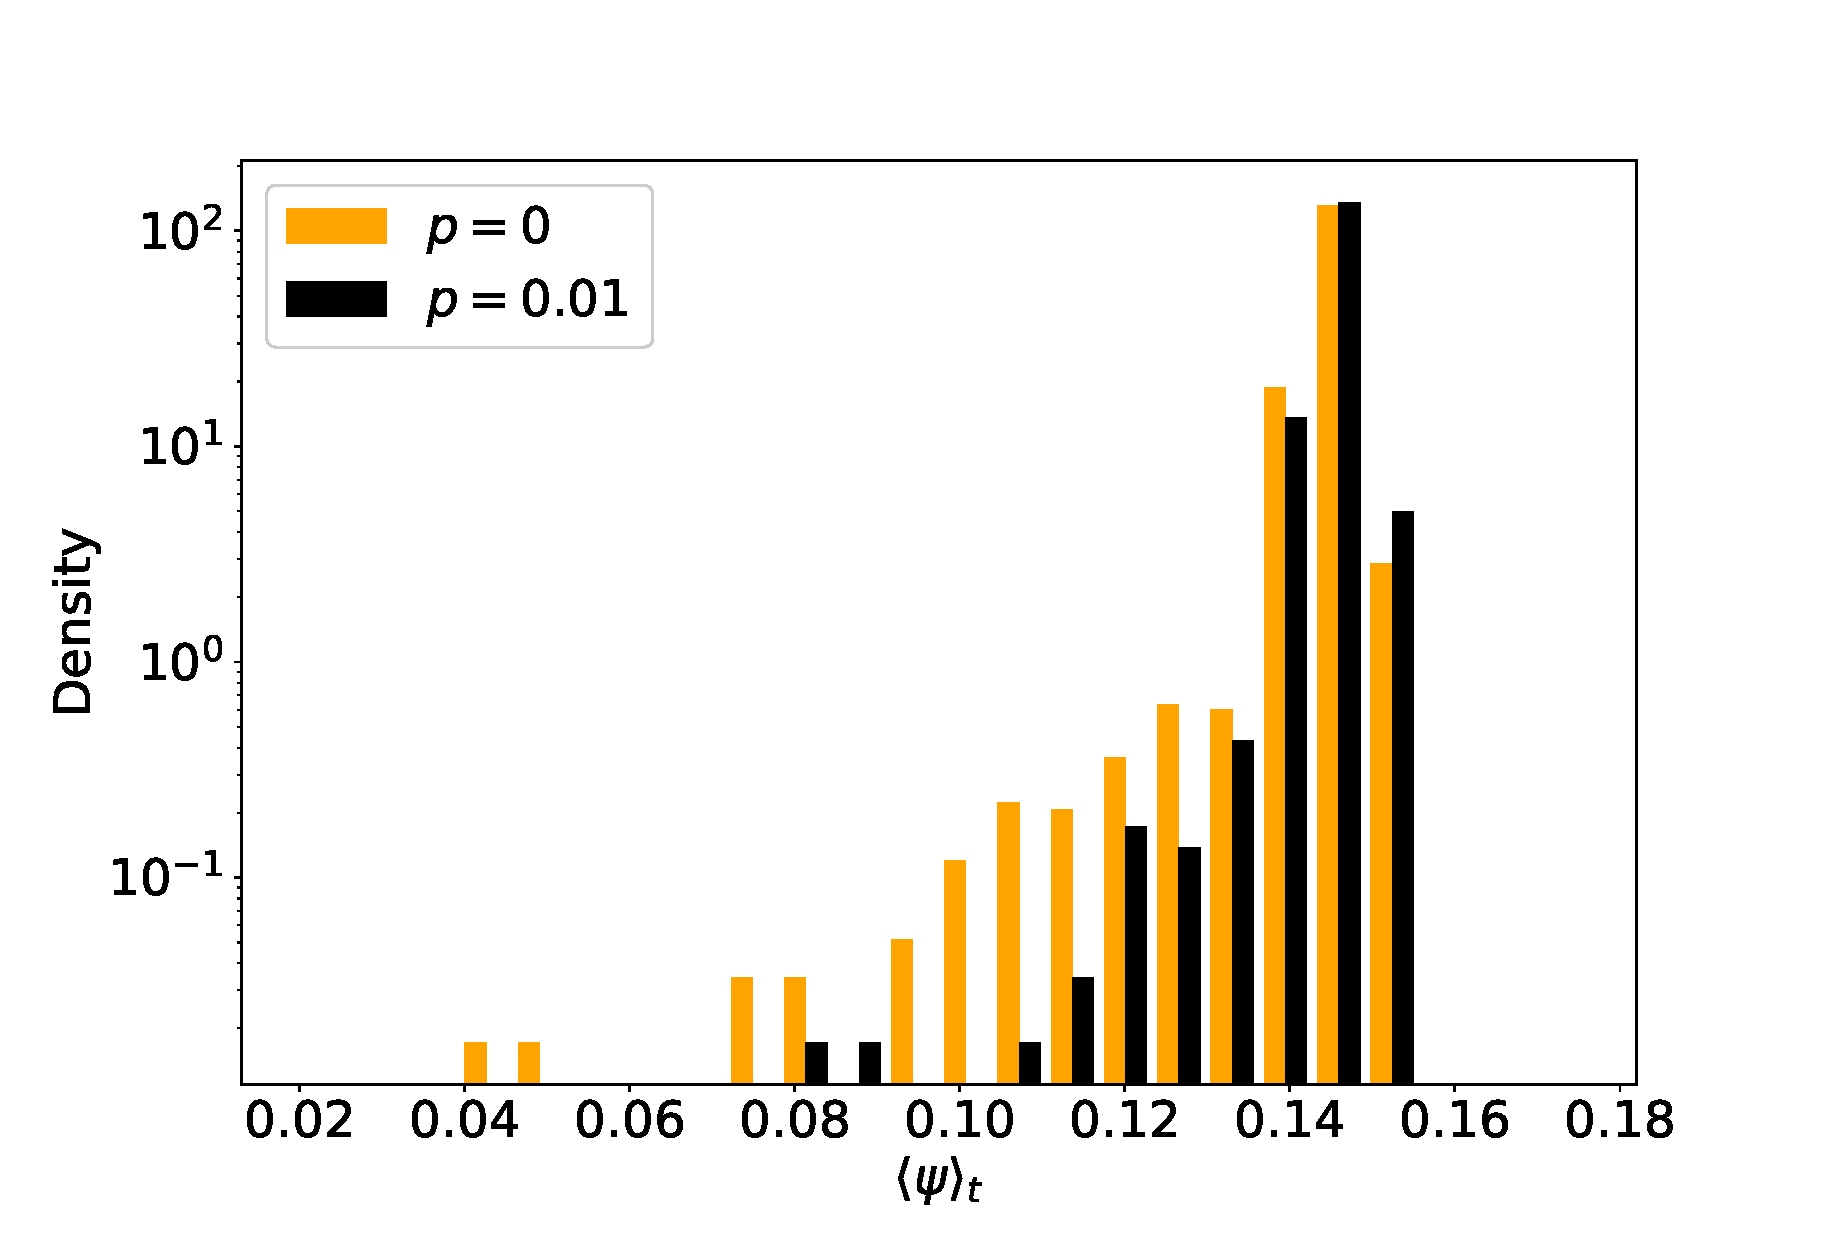
\includegraphics[width=0.8\textwidth]{fig/articuno_figure_histogram.eps}
    \caption{\label{fig:histogram} (Color online) Networks with $N=1000$, $K=129$ and coupling $a=2.5$.  Histograms of $\langle \psi
        \rangle_t$ for 9000 realizations without rewiring (yellow), and 9000 realizations with rewiring probability $p=0.01$ (black).
        The reduced frequency of small order-parameter values for $p=0.01$ compared with $p=0$ is evidence that rewiring destabilizes
        travelling waves, which are characterized by small values of $\psi$.}
\end{center}
\end{figure}

Since rewiring creates long-range interactions that reduce path lengths globally, we expect it to facilitate synchronization. This is
shown to be the case in Fig.~\ref{fig:chicurvespvalue}, where $p$ is gradually increased: realizations starting from \textit{random}
initial conditions are shown to readily synchronize for very small values of $p$, leading to the usual three phases identified for the
complete graph. This means that the introduction of very few global connections is sufficient to destabilize travelling waves; they are
virtually absent for $p \approx 0.01$. In Fig.~\ref{fig:histogram} a histogram of the average order parameter per realization, $\left<
\psi \right>_t$, shows that the fraction of time spent in wave configurations is drastically reduced by the introduction of the
rewiring procedure. When $p\geq0.01$ and $a_c<a<a^c$, the system quickly converges to the  GO phase even if it initially acquired a
wave-like solution (see Fig.~\ref{fig:trialpanel3}). Moreover, if system size is increased at constant $\alpha$, smaller values of $p$
are sufficient to cause the same effect, which is consistent with the fact that the number of long range connections is proportional to
$NK$.

\begin{figure}
\begin{center}
    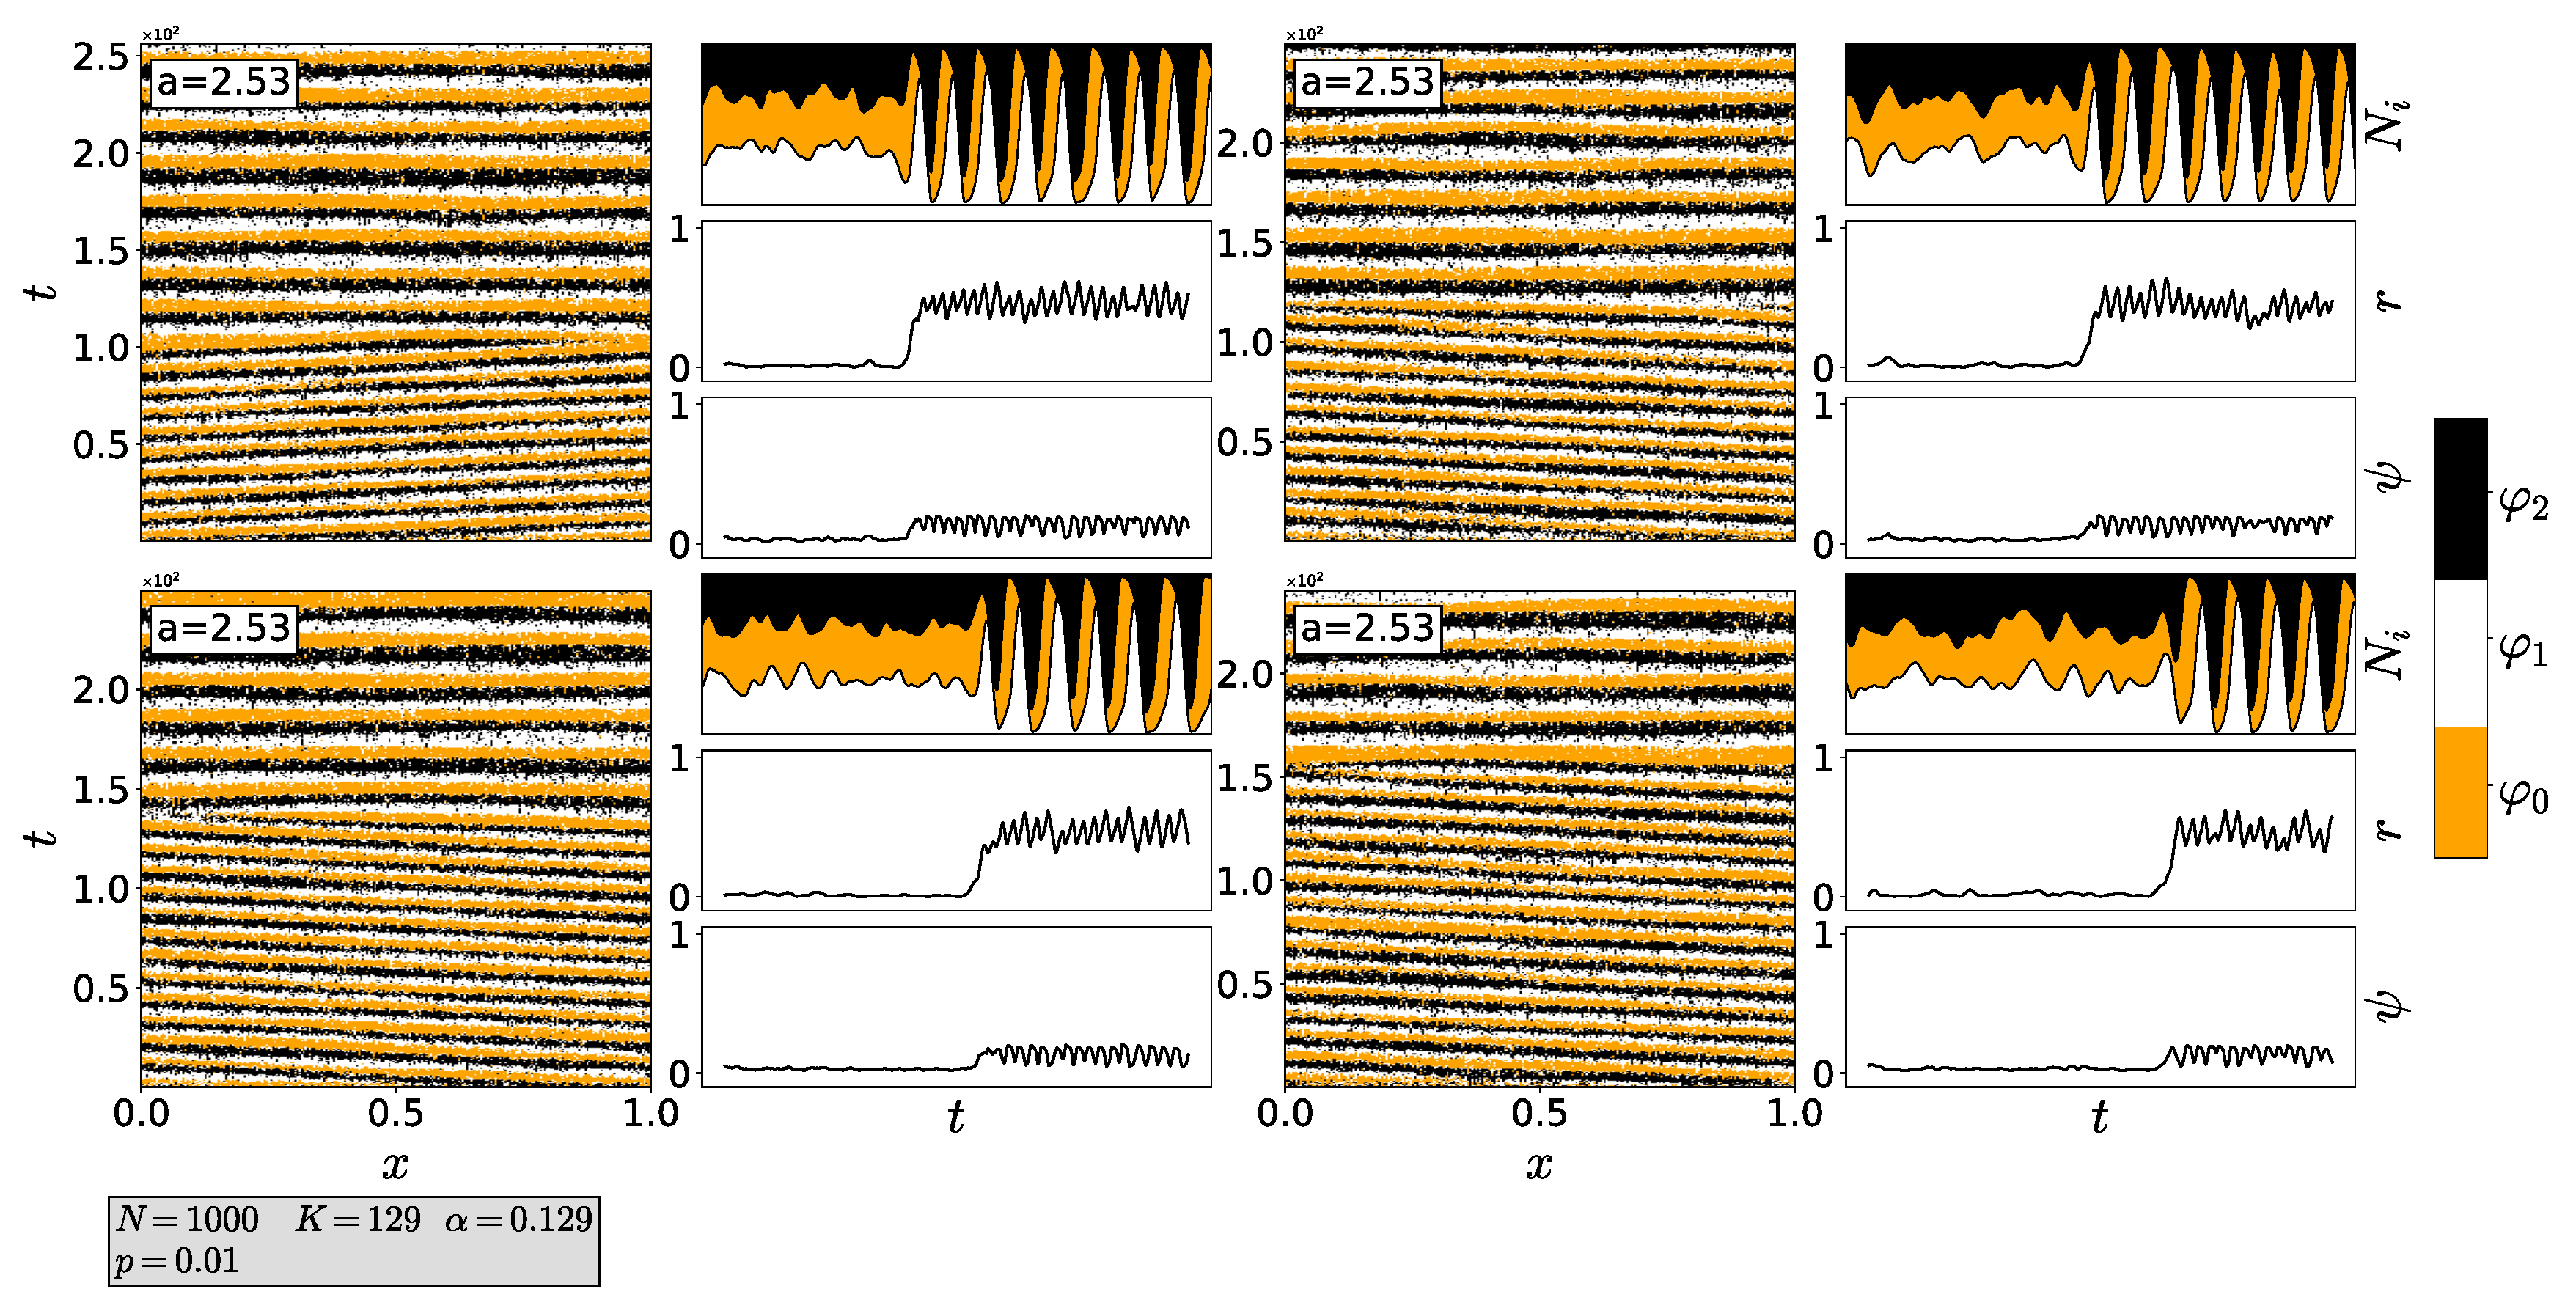
\includegraphics[width=1.0\textwidth]{fig/rewiredwavetrial.eps}
\caption{\label{fig:trialpanel3} Wave states for $N=1000$, $K=129$, $p=0.01$ and $a=2.53$. Only $0.04\%$ of realizations (measured from
9000 realizations) with \textit{random} initial configurations display traveling waves, which are also much more short-lived when compared
to the $p=0$ equivalent system.}
\end{center}
\end{figure}

Following the same procedure as before, we plot in Fig.~ \ref{fig:pvalue} the order parameters versus inverse system size $\lambda$.
Here we fix $\alpha$ at a low value ($\alpha=0.0052$) and vary $p$.  \footnote{{See full animations of figure \ref{fig:pvalue}:
\href{https://youtu.be/3iHXrDUwbqs}{GO transition}},
\href{https://youtu.be/J9OHw3DycAQ}{IP transition}}
Comparing these results with panels d) and h) of Fig.~\ref{fig:opsplit} we see that the mean absolute value of $\psi$ is much greater
when $p$ lies in the small-world region, indicating greater synchrony among oscillators. Space-time plots for values of $p>0$ show that
indeed travelling waves become unstable, so that the system exhibits only the three phases observed on the complete graph, namely,
disordered, GO and IP phases. The phase diagram remains similar to the case of regular rings, displaying low sensibility to $\alpha$
except for very small values where the discreteness of finite systems becomes apparent. The main difference is that for any positive
$p$ wave-like steady states are absent and thus the phase diagram contains only three macroscopically distinct phases.

\begin{figure}
\begin{center}
    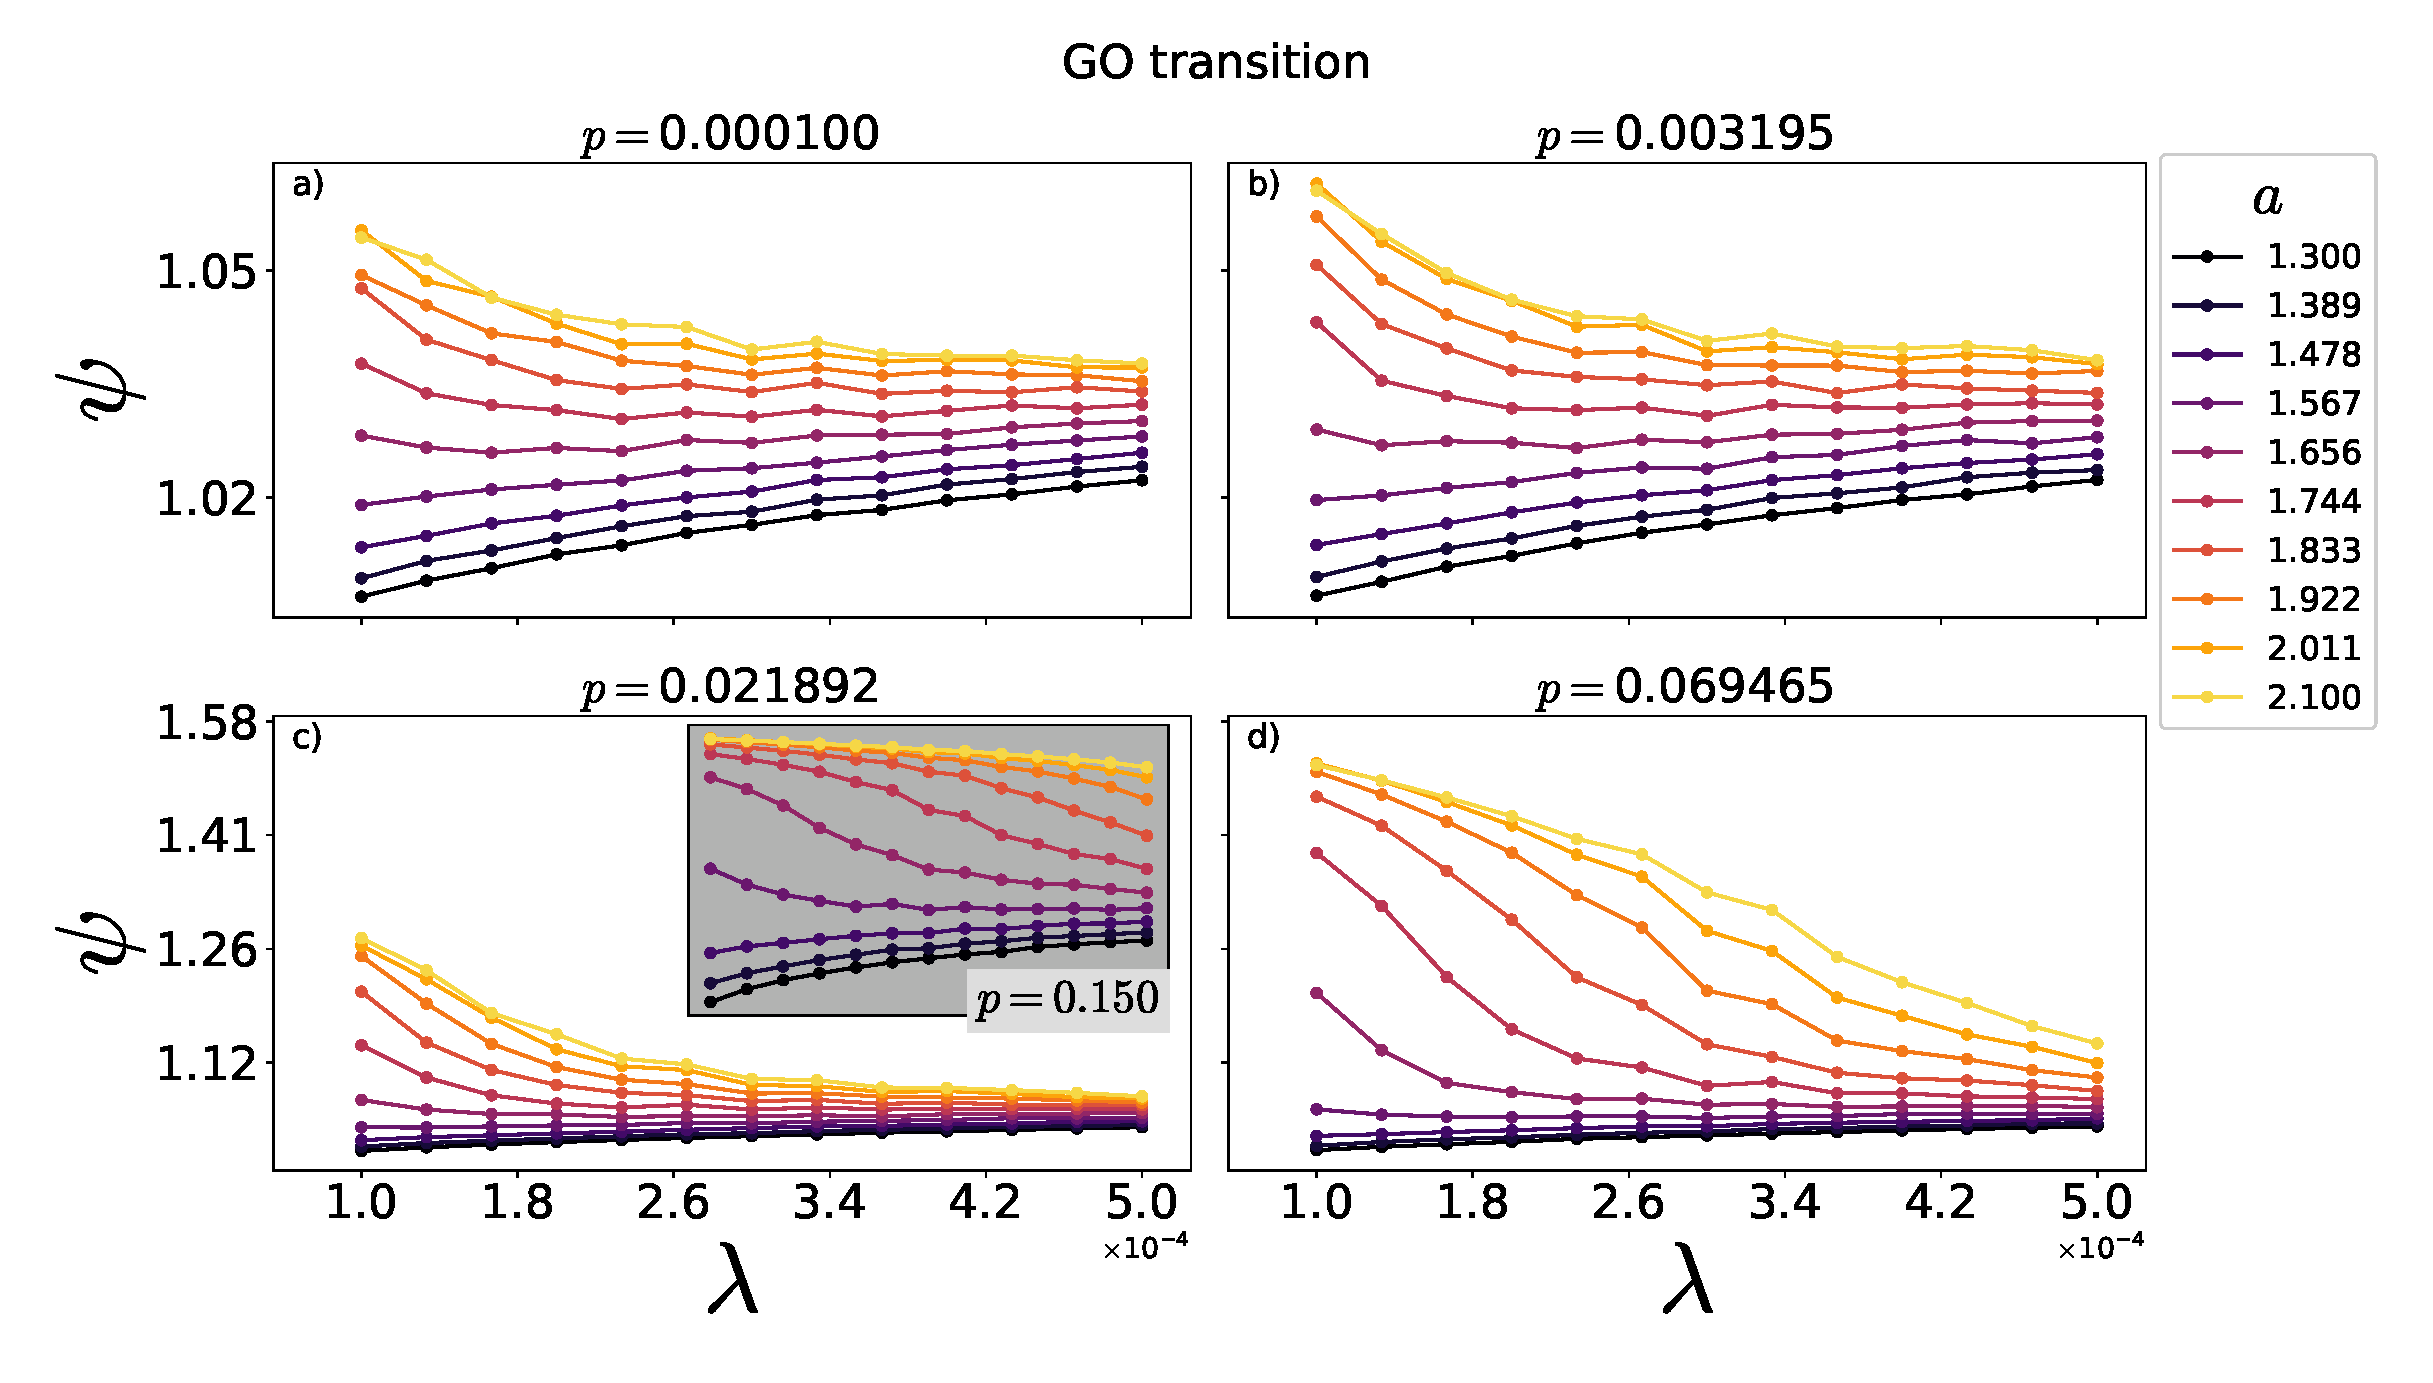
\includegraphics[width=0.9\textwidth]{fig/opsplit-psi-GOT-pvalue.eps}
    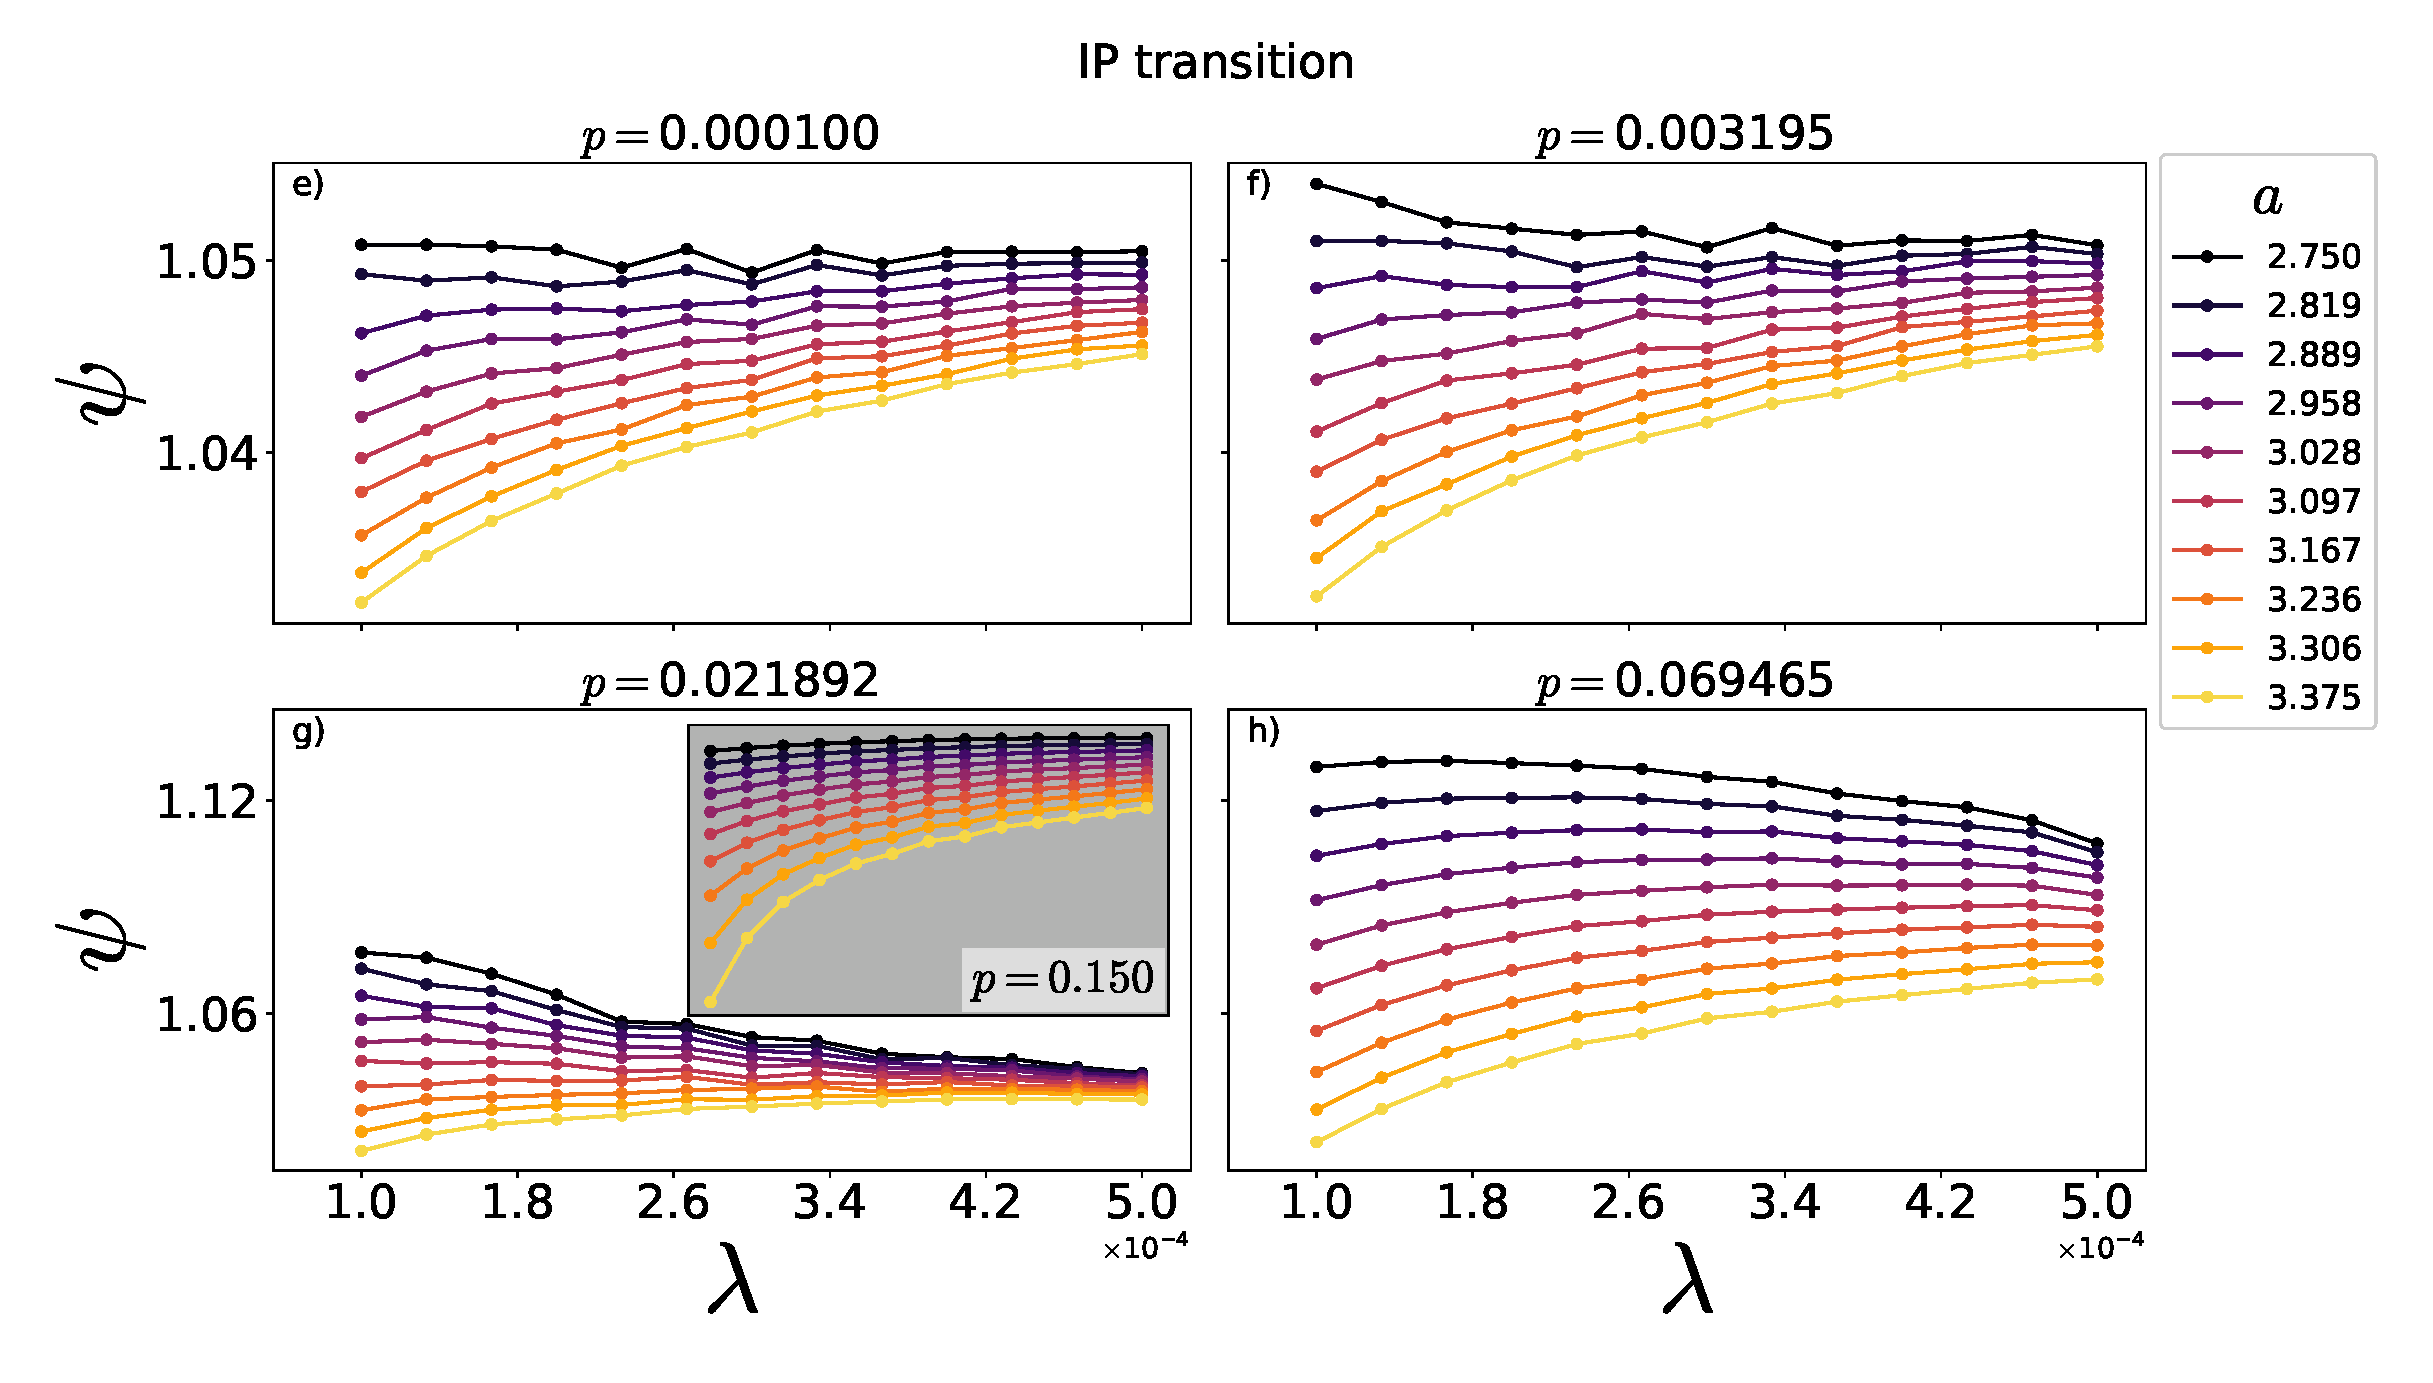
\includegraphics[width=0.9\textwidth]{fig/opsplit-psi-IPT-pvalue.eps}
\caption{\label{fig:pvalue} (Color online) Order parameter $\psi$ versus inverse system size $\lambda$ for $\alpha=0.00524$ and various
values of rewiring probability $p$ and couplings around the GO and IP transitions. Insets show the behavior for $p=0.15$, the highest
rewiring probability used.}
\end{center}
\end{figure}

\clearpage


\section{\label{conclusions}Conclusions}


We study the WCM model, a discrete-phase oscillator model exhibiting global synchronization and an infinite-period phase, on regular
ring lattices and small-world networks.  Each oscillator is coupled to a nonzero fraction $\alpha$ of the others, but the connectivity
is in generally much smaller than for a complete graph.  Our results support the conjecture that all three phases - disordered,
globally synchronized, and infinite-period - appear for any nonzero connectivity $\alpha$. 

Surprisingly, travelling waves also appear in the small-$\alpha$ regime on regular ring lattices;  such waves may represent a
long-lived metastable state.  (A previous study identified waves in the anti-coupling case \cite{escaff2014arrays}.) In our studies
travelling waves constitute only about $1.6\%$ of the steady states reached from starting from \textit{random} initial configurations,
and are prone to decay into global oscillations due to fluctuations when system size is small.  The introduction of long-range
interactions through rewiring (i.e., using the Watts-Strogatz algorithm) can lead to synchronization without increasing the total
number of connections.  Rewiring also suppresses travelling waves by introducing long range interactions.

The fact that regular rings are capable of sustaining travelling waves for $a>a_c$ is surprising, showing that networks of oscillators
might fail to synchronize even in the presence of nonlocal interactions and strong coupling, conditions which are sufficient for the
synchronization on hypercubic lattices of dimensions greater than 2 as well as on the complete graph. This raises the possibility that
WMCs admit wave-like steady states on cubic lattices, similar to oscillations observed in the two-dimensional Belousov–Zhabotinsky
reaction.

Several other questions remain open for future study, for example, whether travelling waves represent a stable phase for some range of
parameters, or are always metastable, and whether waves of wavelength smaller than the system size $N$ are possible.  We have sketched
a phase diagram for ring lattices, but detailed information for the small-connectivity regime is lacking.  Since the model exhibits a
pair of continuous phase transitions, it is of interest to develop a full scaling picture, including the effect of ordering fields
conjugate to the order parameters.  Finally the question of what simple external  perturbations are capable of destroying
synchronization or the symmetry-broken phase may be of some practical interest.


\chapter{Mean-field theory for small-world networks}
\label{chap:mf}

%The previous chapter focused mainly on simulation results for ring-lattices and small-world networks.

In this chapter we develop a mean field (MF) theory for the coupled oscillator dynamics with three discrete phase states in a system of
$N$ oscillators coupled in small-world networks as described by the Watts-Strogatz algorithm in section~\ref{smallworld}. We start by
re-stating the dynamic rules, and then proceed to define the mean field and the continuous limit.

\begin{table}[ht] 
  \centering
  \caption{Definitions}
  \resizebox{\linewidth}{!}{%
  \bgroup
  \def\arraystretch{1.4}  % increase row padding
  \begin{tabular}{|c|l|}
    \hline
  $N$ & Integer system size \\ \hline 
  $K$ & Integer interaction range \\ \hline 
  $a$ & Real coupling strength, $a\geq 0$\\ \hline 
  $\alpha$ & Interaction range as a fraction of system size $\alpha\equiv K/N$\\ \hline 
  $p$ & Rewiring probability\\ \hline 
  $\gamma_j^x(t) | \gamma_j(x,t)$ & Transition rate out of state $j$ at position $x$ and time $t$\\ \hline 
  $P_j^x(t) | P_j(x,t)$ & Probability that an oscillator at $x$ is in state $j$ at time $t$\\ \hline 
  \end{tabular}%
  \egroup
  }
\end{table}

An oscillator is described by its discrete phase, which can be imagined as a clock hand which abruptly jumps from noon to 4pm, then to
8pm and back to noon. Note that, as in a clock, the phase can only move forward, looping back on itself after three jumps.  These jumps
occur randomly, but with a well defined transition rate. When two oscillators interact, the rate of transition may change depending on
the relative phase between the two units.

To describe the phase and interactions, we adopt a convention: oscillators are arranged in a circle and numbered from 1 to $N$ (see
figure~\ref{fig:ring-distance}). The superscripts then refer to the oscillator position while the subscripts denote a phase state from
1 to 3. Given a graph in which nodes represent phase oscillators labeled by $x$, the unit at position $x$ is described by its phase

\begin{align}
  \phi^x = 2\pi (j-1)/3 \\
  j \in \{1,2,3\} \notag
\end{align}

\noindent where $j\in\{1,2,3\}$ is the state of unit $x$. Since transitions can only occur in one direction, the stochastic rate of
transition from $j$ to $j+1$ is written just as $\gamma^x_j$, and its behavior is chosen to be of an exponential form:

\begin{equation}
  \gamma^x_j(t) = \omega^x\exp\left[ a\frac{n^x_{j+1}(t) - n^x_j(t)}{n^x} \right] \qquad x=1,\dots, N
  \label{eq:rate}
\end{equation}

\noindent where $\omega^x$ is its natural (uncoupled) frequency, $n^x_j(t)$ is the count of how many of its neighbors are in state $j$,
and $n^x$ is its total number of neighbors.

Let the probability of finding the unit at position $x$ in state $j$ at time $t$ be $P_j^x(t)$. Since there are only three possible
states we have the constraints $P_1^x(t)+P_2^x(t)+P_3^x(t)=1$ for all $x$ and $t$. The rate of change of the probabilities can be
written in terms of the transition rates $\gamma^x_j(t)$, giving us $2N$ equations of motion:

\begin{align}
  \ddt{p}^x_1(t) &= \gamma^x_3(t)(1 - P_1^x(t) - P_2^x(t)) - \gamma^x_1(t) P_1^x(t) & \notag\\
  \ddt{p}^x_2(t) &= \gamma^x_1(t)P_1^x(t) - \gamma^x_2(t) P_2^x(t) &x=1,\dots,N
  \label{eq:motion}
\end{align}

\noindent The first terms in the RHS of (\ref{eq:motion}) represent the fluxes of probability from oscillators in the preceding state,
which can advance one phase state and increase the populations of oscillators in states 1 and 2 respectively. The second (negative)
terms represent the fluxes generated by the oscillator leaving the considered state, and thus reducing its population. The dynamics can
take place on any arbitrary network that defines the coupling between oscillators. Previous work has explored hyper-cubic lattices and
complete graphs as well as regular ring graphs \cite{Wood06a,assis2011infinite,escaff2014arrays}.

Here we start by focusing on ring lattices, which will be the starting point for generating small-world networks. Ring lattices are
constructed by arranging $N$ oscillators in a circle, and then for each unit, adding $K$ clock-wise connections to the next $K$ units
in the circle, resulting in a circular shape with $NK$ total connections. The result of this process for $N=12$ and $K=2$ is shown in
figure~\ref{fig:ring} of chapter~\ref{chap:article}, as well as for $N=16$, $K=2$ in figure~\ref{fig:ring-distance} right.

To generate a small-world network from a ring graph we perform a \textit{rewiring} procedure. It visits each existing connection
exactly once, and with a probability $p$ exchanges the clockwise vertex of this connection for a randomly selected node in the network,
avoiding duplicate connections or self connections. This will be described in detail when deriving the MF approximation for small-world
networks.

\section{The local average field in the discrete case}

To define the local average field, we introduce a \textit{local order parameter} $\nu$ identified by the fractions in the exponent of
equation~(\ref{eq:rate}) at a fixed time $t$. It is a measure of the synchrony between oscillators which are coupled to the
oscillator at position $x$.

\begin{equation}
  \nu^x_j(t) \equiv \frac{n^x_j(t)}{n^x},
\end{equation}

\noindent the transition rates are now written as,

\begin{align}
  \gamma^x_j(t) = \omega^x\exp\left[ a(\nu^x_{j+1}(t) - \nu^x_j(t)) \right].
  \label{eq:mfrate}
\end{align}

The quantity $\nu^x_j$ describes the fraction of oscillators connected to $x$ that are in state $j$, and thus also satisfies the
constraint $\nu^x_1+\nu^x_2+\nu^x_3=1$.

In the large-$N$ limit, we approximate $\nu^x_j$ in equation~(\ref{eq:mfrate}) by its time-dependent average over realizations, $\left<
\nu^x_j(t) \right>$. When the rewiring probability $p=0$, it was shown that for the chosen form of the coupling, the variance
$\text{Var}[\nu^x_j]$ is proportional to $1/N$ \cite{escaff2014arrays}. In the case of small-world networks ($0<p \leq 1$) it is
unfeasible to explicitly calculate the variance of the local order parameter, but in section~\ref{subsection:justifyapproximations} we
develop arguments that support the validity of this mean-field approximation by performing partial calculations, and in
chapter~\ref{chap:simulation} we also perform numerical simulations for finite systems.

If fluctuations are small compared to the deterministic drift described by the MF approach the assumptions become better, but a
quantitative description may suffer from imprecision when compared to simulation results. With this in mind, the MF transition rates
become:

\begin{align}
  \gamma^x_{j,MF} = \omega^x \exp \left[ a \left( \left< \nu^x_{j+1}(t) \right> - \left< \nu^x_j(t) \right> \right) \right]
  \label{gammaMF}
\end{align}

For regular rings, the total number of neighbors of every site is fixed, $n^x= 2K$, but when dealing with rewired networks $n^x$
becomes a random variable which may assume different values in different realizations, making $\left<\nu^x_j(t)\right>$ trickier to
calculate.

The equations of motion in the MF approximation are obtained by replacing the instantaneous transition rates in equation~
(\ref{eq:motion}) by their mean-field values.

\begin{align}
  \ddt{P_1^x}(t) &= \gamma^x_{3,MF} (1-P_1^x(t)-P_1^x(t)) - \gamma^x_{1,MF} P_1^x(t) \notag \\
  \ddt{P_2^x}(t) &= \gamma^x_{1,MF}  P_1^x(t) - \gamma^x_{2,MF} P_2^x(t)
  \label{eq:motionmf}
\end{align}

We are left with the task of calculating $\left<\nu^x_j(t)\right>$ in terms of the probabilities $P^x_j(t)$ such that \ref{eq:motionmf}
is an autonomous system. For that we define the indicator variable $D^{xx'}$, indicating the presence (or absence) of coupling between
nodes $x$ and $x'$ in a graph.

\subsection{Mean field value of the local order parameter}

The expressions for $\nu^x_j(t)$ in the discrete case can be written in terms of the indicator variables $D^{xx'}$:

\begin{itemize}
  \item Let $D^{xx'}$ be defined as
  \begin{align}
  D^{xx'} = 
    \begin{cases}
    1 \qquad &\text{if the connection $x$,$x'$ exists}\\
    0 \qquad &\text{otherwise}
    \end{cases}
  \end{align}
  \item Let $x$ denote some position in the lattice for which we wish to know the local order-parameter value.
  \item Let $j$ denote the state for which we wish to measure $\nu^x_j$.
\end{itemize}

\noindent Then:

\begin{align}
  n^x_j(t) &= \sum\limits_{x'=1}^ND^{xx'}\delta(j,j'(t)) \notag\\[8pt]
  n^x &= \sum\limits_{x'=1}^ND^{xx'}
\end{align}

\noindent where $j'$ is the state of the oscillator at position $x'$ at time $t$ and $\delta(j,j'(t))$ is the usual Kronecker delta
defined by $\delta(j,j')=1$ if $ j=j'$ and $0$ otherwise. The average over realizations then become

\begin{equation*}
  \left< \nu^x_j(t) \right> = \sum_{x'} \left< \frac{D^{xx'}\delta(j,j'(t))}{\sum_{x''}D^{xx''}} \right>,
\end{equation*}

\noindent or,

\begin{equation}
  \left< \nu^x_j(t) \right> = \sum_{x'} \left< \frac{D^{xx'}}{\sum_{x''}D^{xx''}}\right>\left<\delta(j,j'(t)) \right>.
  \label{eq:numf}
\end{equation}

\noindent Equation~(\ref{eq:numf}) introduces the principal MF approximation, treating $\delta(j,j'(t))$ as independent of $D^{xx'}$,
implying the dynamics is described by the ``average connectivity'' between oscillators on the graph. This approximation becomes more
accurate when the probability of rewiring $p$ approaches zero, which is true for a large number of networks in the small-world regime,
as seen in figure~\ref{fig:small-world} of chapter~\ref{chap:article}. When $p=0$ we can restrict the summation over connected sites,
from $(x-K)$ to $(x+K)$, recovering the MF proposed by Escaff \textit{et al.}~\cite{escaff2014arrays} for regular rings.

The average $\left< \delta(j,j'(t)) \right>$ is identified with the probability of finding site $x'$ in state $j$ at time $t$: $\left<
\delta(j,j'(t)) \right> \equiv P_j^{x'}(t)$, and we are left with the task of calculating $\left< D^{xx'}/\sum D^{xx'} \right>$. In
order to unpack this expression we need a detailed description of the rewiring algorithm, which ultimately dictates the connectivity of
the final graph.

\begin{figure}
  \centering
  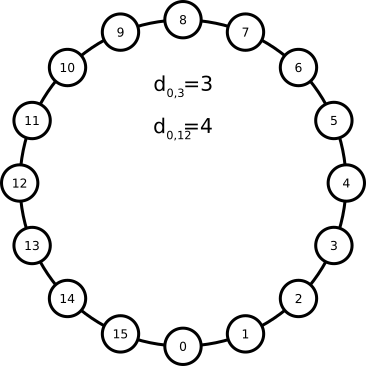
\includegraphics[width=0.75\textwidth]{fig/ring-distance.png}
  \caption{\label{fig:ring-distance}
    \textbf{Left:} Definition of distance $d_{xx'}$ between sites $x$ and $x'$. The distance $d_{xx'}$ is considered on the one
    dimensional chain and does not take into account the connections that determine the coupling.\\
    \textbf{Right:} Example of the initial ring lattice before any rewiring is performed, where the lines represent the coupling
    between units.\\
    The dynamics takes place on a periodic one-dimensional system with interaction range $K$.
  }
\end{figure}

\subsection{Rewiring algorithm}

Here we give a detailed description of the rewiring algorithm in order to justify our expressions for the probability of connections in
the final graph, which dictate the dynamics. It considers each connection in the starting graph exactly once, and with probability $p$
it tries to swap one of its vertices for another randomly selected node in the network, avoiding double connections or
self-connections. Detailed instructions on how it is implemented are written in the following pseudo-code.

\noindent
\begin{minipage}{\linewidth}
\begin{lstlisting}
Given a ring lattice with N nodes and range K do:
for z from 1 to K:
  for x from 1 to N:
    with probability p do:
      sample a uniform integer r from 1 to N
      if ( r == x ) or ( connection (x, r) already exists ):
        do nothing
      else:
        remove the connection (x, x+z)
        add the connection (x, r)
\end{lstlisting}
\end{minipage}

To determine the probability that the connection $(x, x')$ exists in the rewired graph, we introduce the notion of distance between
nodes $x$ and $x'$. Let this be denoted by $d_{xx'}$, and the distance defined in the one-dimensional chain as illustrated in
figure~\ref{fig:ring-distance}. Due to the periodic condition $x \mapsto x+N$ on the boundaries, no distance can be greater than $N/2$,
and thus $d_{xx'}$ is formally defined as:

\begin{align}
  d_{xx'} =
  \begin{cases}
    |x-x'| \quad &\text{if $|x-x'|\leq N/2$} \\
    N-|x-x'| \quad &\text{if $|x-x'| > N/2$}
  \end{cases}
  \label{dist}
\end{align}

To calculate the average values $\left< D^{xx'} \right>$ we consider two cases: $d_{xx'} \leq K$, the \textbf{close case}, and $d_{xx'}
> K$, the \textbf{far case}. The reasoning is that:

\begin{itemize}
  \item If the initial distance between two nodes is less than or equal to $K$, then by construction of the ring graph they start out
    connected. The condition that this connection exists in the final graph is that it was never removed in the first place, or it
    could have been removed and then subsequently reformed.

  \item On the other hand, sites with $d_{xx'}>K$ start out disconnected, and thus a connection $(x,x')$ can only result from one of
    its vertices being rewired that way.
\end{itemize}

With a little thought regarding the rewiring procedure, one will agree that if it produces any connection, it is guaranteed to be
present in the result. Conversely, if it fails to break an initial connection, that connection is also guaranteed to exist in the final
graph.

\subsection*{Far case}

\begin{figure}
  \centering
  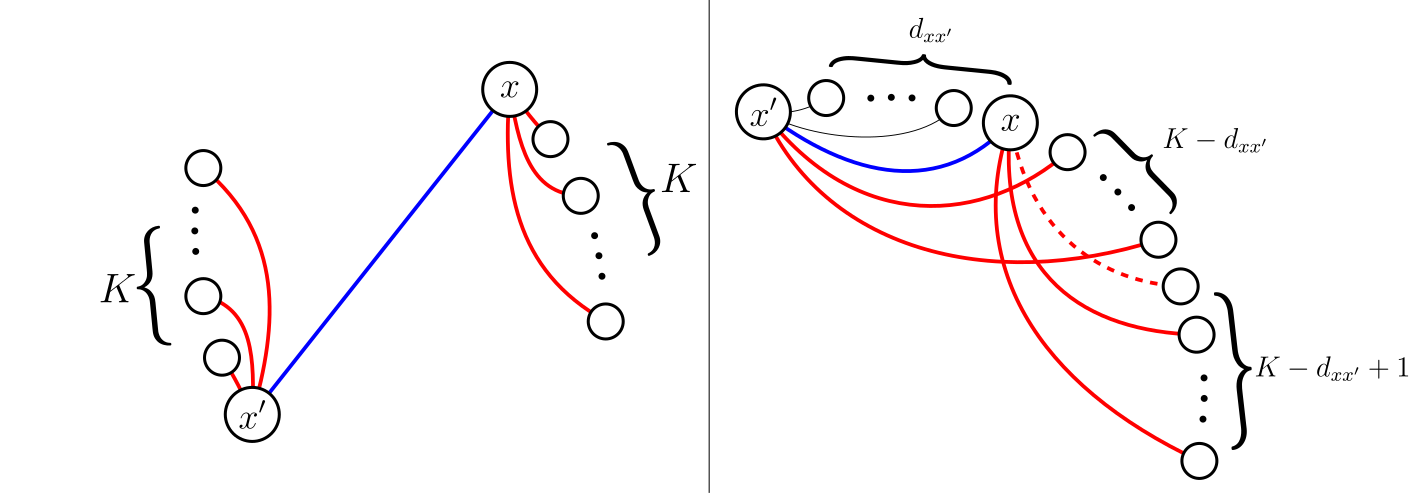
\includegraphics[width=0.9\linewidth]{fig/rewire_contributions.png}
  \caption{The presence of the connection $(x,x')$, in {\color{blue}\textbf{blue}}, in a small-world network generated from the
    Watts-Strogatz algorithm can only be the result of the rewiring of a {\color{red}\textbf{red}} connection. On the left side, the
    \textbf{far} case, $2K$ connections may contribute to the formation of $(x,x')$. On the \textbf{near} case (right side), the
    original connection may either be left untouched or, in case it is initially broken, it might be wired again by any of the
  remaining $2(K-d_{xx'})+1$ solid {\color{red} red} connections.}
  \label{fig:rewire_contributions}
\end{figure}

Here we derive the probability of existence of a connection between $x$ and $x'$ when $d_{xx'}>K$. Since the algorithm tries to swap
(with probability $p$) the clockwise node of an initial connection, the only connections that could possibly have broken to form
$(x,x')$ are the $K$ clockwise neighbors of $x$, and the $K$ clockwise neighbors of $x'$, as illustrated in the left panel of
figure~\ref{fig:rewire_contributions}. If any of these $2K$ events take place, $(x,x')$ is guaranteed to exist. Thus, $P(D^{xx'}=1)$ is
the probability that at least one forming event took place, which is just the complement of the probability that \textit{no} such event
took place.

\begin{align}
  P(D^{xx'}=1) = 1 - \left( 1 - \frac{p}{N} \right)^{2K} \qquad \text{for} \quad d_{xx'} > K
  \label{eq:probfar}
\end{align}

In equation~(\ref{eq:probfar}), the probability that a connection rewires to $(x,x')$ is the probability that it breaks times the
probability of selecting the other vertex, which is just $p/N$. Therefore, the probability that a connection \textit{does not} rewire
to $(x,x')$ is the complement $1-p/N$. The probability that \textit{none} of the $2K$ connections generate $(x,x')$ is then
$(1-p/N)^{2K}$, and the probability that at least one of them \textit{does} generate it is the complement again.

\subsection*{Near case}

The near case is given by $d_{xx'}\leq K$. When considering the probability of existence for such shorter range connections, things get
more complicated because the exact solutions depend on the choice of the starting point of the rewiring procedure. Consider the case
shown in figure~\ref{fig:order_dependence} for interaction range $K=1$.

\begin{figure}[!ht]
  \centering
  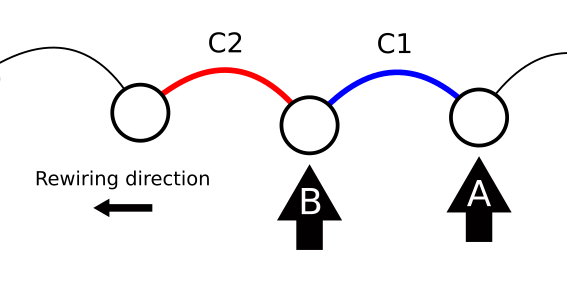
\includegraphics[width=0.7\linewidth]{fig/order_dependence.png}
  \caption{Rewiring of connection C2 may or may not contribute to the probability of existence of connection C1. If the rewiring
  process starts at A, then C2 may be rewired into C1 if it was initially broken. On the other hand, if the starting point is B,
  connection C2 can never be rewired to C1 because the later will always be present at the time of rewiring C2.}

  \label{fig:order_dependence}
\end{figure}

If the rewiring process starts at point A, then rewiring of connection C2 contributes to the probability that C1 is present in the
final graph. On the other hand, if the rewiring starts at point B, then C2 does not contribute to the probability of existence of C1.
Therefore C1 has a higher probability of existing for a rewiring that started at A as opposed to one that started at B. Luckily for our
purposes the order dependence only happens for the first connection of length $d_{xx'}$ (dashed {\color{red}red} line on right of
figure~\ref{fig:rewire_contributions}), since for subsequent connections (solid {\color{red}red} lines on same figure) the pair
$(x,x')$ will already have been considered by the algorithm, and any forming event from that point guarantees the existence of the
connection $(x,x')$.

To avoid order dependence, we will assume the problematic event contributes the same amount as subsequent events to the probability of
existence of the considered connection. Thus, all $2K-2d_{xx'}+1$ events contribute equally to $P(D^{xx'}=1)$, which is written as:

\begin{align}
  P(D^{xx'}=1) = 1 - p\left(1-\frac{2K}{N}\right)\left(1-\frac{p}{N}\right)^{2K - 2d_{xx'} + 1} \qquad \text{for} \quad d_{xx'} \leq K
  \label{eq:probnear}
\end{align}

\noindent As before, the expression is obtained by taking the complement of the probability that no event forms the connection
$(x,x')$: the probability that the original connection is broken is $p(1-2K/N)$ ($p$ times the probability of selecting a site which
does not already have a connection with $x$). This is another approximation since the number of connections involving site $x$ may
change during the rewiring procedure, but because the later conserves the total number of connections it is at least justifiable for
now (we later confirm it numerically). The term $(1-p/N)^{2K-2d_{xx'}+1}$ accounts for the probabilities that no forming event occurs
with the potential connections marked in {\color{red}red} on the right side of figure~\ref{fig:rewire_contributions}.

\subsection{The discrete average field}
\label{subsection:justifyapproximations}

\begin{figure}
  \centering
  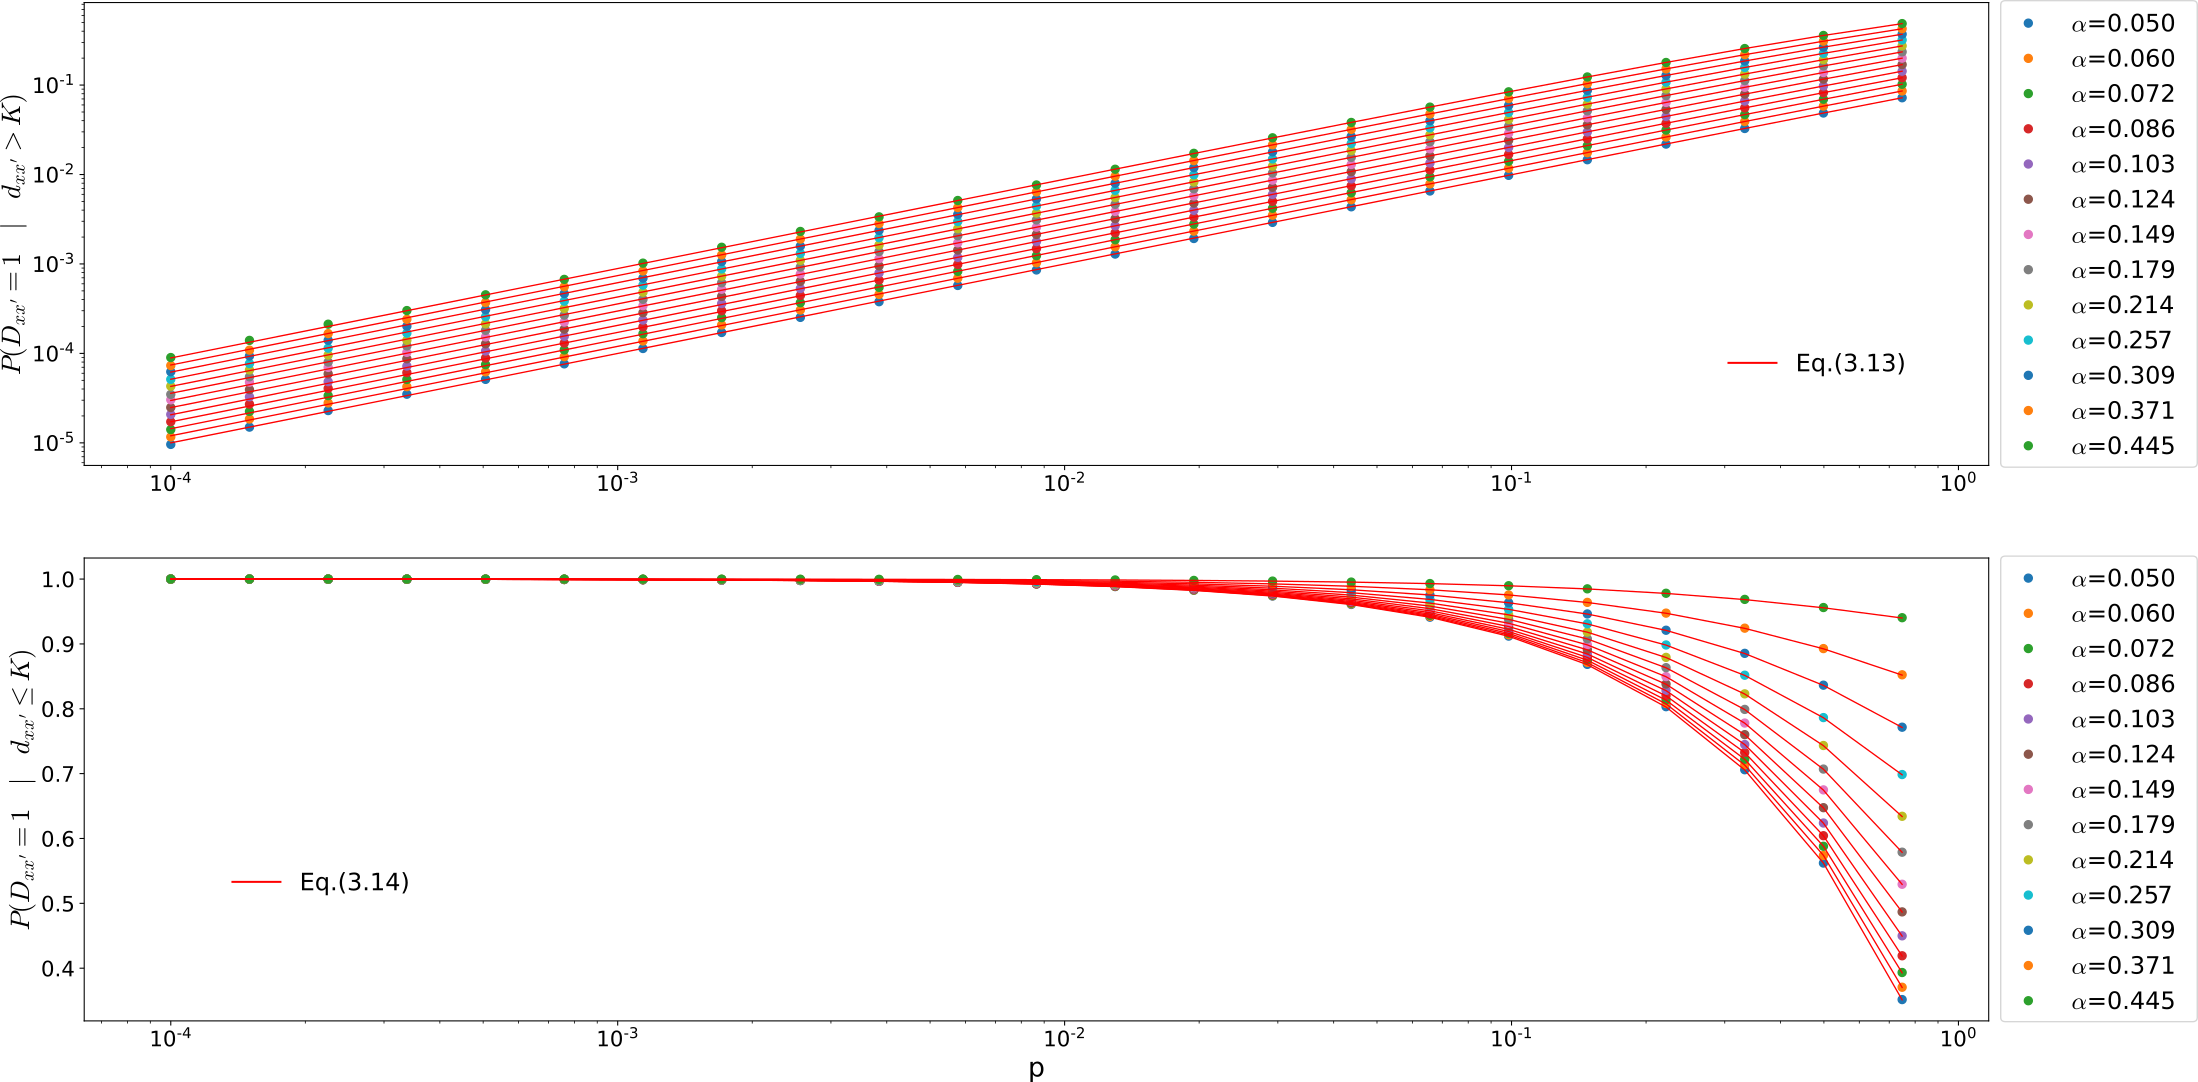
\includegraphics[width=\linewidth]{fig/rewire_mc.png}
  \includegraphics[width=\linewidth]{fig/chap3/mcerror.png}
  \caption{
		Comparison between expressions for the probability of existence of connections as functions of rewiring probability $p$.  Dots are
		obtained from Monte Carlo sampling of small-world networks produced by the Watts-Strogatz algorithm, solid red lines are equations
		(\ref{eq:probfar}) (top) and (\ref{eq:probnear}) (bottom). \\ System size $N=1000$ with 50 realizations each. Note that when $p\to
		0$ initially disconnected oscillators remain uncoupled while oscillators at distances $d^{xx'}\leq K$ remain coupled.  The last two
		graphs depict the percentage deviation between sampling and predicted values, which is under 6\% for connections longer than $K$
		and under 0.2\% for shorter range connections.
	}
  \label{fig:rewire_mc}
\end{figure}

To check that the probabilities $P(D^{xx'})$ are valid, we performed Monte Carlo sampling of the small-world networks and plotted the
relative frequencies obtained against the probabilities given by equations~(\ref{eq:probfar}) and (\ref{eq:probnear}). The results are
shown for various values of $p$ and $\alpha \equiv K/N$ in figure~\ref{fig:rewire_mc}, where good agreement is observed for all values
of $p$ and interaction range $K$ with fixed $N=1000$.

Note that since $D^{xx'}$ are binary variables with values 1 and 0 the probabilities $P(D^{xx'}=1)$ are given by the average
$\left<D^{xx'}\right>$, resulting in

\begin{equation}
  \left<D^{xx'}\right> =
  \begin{cases}
    1-\left( 1 - \frac{p}{N} \right)^{2\alpha N} \quad &\text{if} \quad d_{xx'}>K \\
    1-p\left( 1 - 2\alpha \right)\left( 1 - \frac{p}{N} \right)^{2(\alpha-\alpha')N+1} \quad &\text{if} \quad d_{xx'}\leq K\\
  \end{cases}
  \label{eq:probconnection}
\end{equation}

\noindent where we have used the definitions $\alpha \equiv K/N$ and $\alpha' \equiv d^{xx'}/N$, which are assumed to be constant as
$N$ scales with proportional $K$ and $d^{xx'}$. When $N$ is large, we use the property

\begin{equation*}
  \lim_{N\to \infty}\left( 1 - \frac{p}{N} \right)^{2\alpha N + C} = e^{-2\alpha p}
\end{equation*}

\noindent to simplify the expression to

\begin{equation}
  \left<D^{xx'}\right> =
  \begin{cases}
    1-e^{-2\alpha p} \quad &\text{if} \quad d_{xx'}>K \\
    1-p\left( 1 - 2\alpha \right)e^{-2(\alpha-\alpha')p} \quad &\text{if} \quad d_{xx'}\leq K\\
  \end{cases}
  \label{eq:probconnectionexp}
\end{equation}

Going back to equation~(\ref{eq:numf}), we wish to calculate the quantity $\left< \frac{D^{xx'}}{\sum D^{xx'}} \right>$. To do this, we
argue that $\var{\sum D^{xx'}}$ is small, and thus $\sum D^{xx'} \simeq \left< \sum D^{xx'} \right>$ which is a constant, allowing us
to replace the average of the quotient by the quotient of the averages, leading to

\begin{equation}
    \left< \frac{D^{xx'}}{\sum_{x'}D^{xx'}} \right> \simeq \frac{\left< D^{xx'} \right>}{\sum_{x'}\left< D^{xx'} \right>}
    \label{eq:avgquotient}
\end{equation}

\noindent For small-world networks, the parameter $p$ tends to be small\cite{rodrigues2020synchronization}, as seen from
figure~\ref{fig:small-world}. Thus, we take equation~(\ref{eq:probconnectionexp}) and expand the exponential terms in powers of $p$
around $p=0$. Keeping up to first order in $p$ results in:

\begin{align}
  \sum_{x'=1}^N \left< D^{xx'} \right> = &
  \sum_{d_{xx'}>K} 2\alpha p \notag \\
  + &
  \sum_{d_{xx'}\leq K} \left( 1 - p + 2\alpha p \right),
\end{align}

Since the terms are now independent of $x'$, and noting that there are $2K=2\alpha N$ terms with distance $d^{xx'}\leq K$ and
$N-2K=N(1-2\alpha)$ terms with distance $d^{xx'}>K$, we obtain:

\begin{align*}
  \sum_{x'=1}^N \left< D^{xx'} \right> &\simeq N(1-2\alpha)2\alpha p + 2\alpha N\left( 1 - p + 2\alpha p \right) \\
	\intertext{\noindent which cancels out as}
  &= \cancel{2\alpha Np} - \bcancel{4\alpha^2Np} + 2\alpha N - \cancel{2\alpha Np} + \bcancel{4\alpha^2Np}
\end{align*}
\noindent giving,
\begin{align}
  \sum_{x'=1}^N \left< D^{xx'} \right> &\simeq 2K
\end{align}

This result is consistent with the previous statement that the average
number of neighbors remains unchanged after the rewiring procedure, and also recovers previous results\cite{escaff2014arrays} for the
case $p=0$.

We now focus briefly on calculating $\var{\sum D^{xx'}}$. The numerical analysis depicted in figure~\ref{fig:rewire_mc} shows that
regarding the presence of connections in the final graph as independent events is a very good approximation. Thus, we can distribute
the variance function inside the summation and ignore the covariance term, leading to:

\begin{equation}
  \var{\sum_{x'}D^{xx'}} = \sum_{x'} \var{D^{xx'}}
\end{equation}

\noindent where $\var{D^{xx'}} = \left< \left( D^{xx'} \right)^2 \right> - \left< D^{xx'} \right>^2$, but since $D^{xx'}$ are indicator
variables with outcomes 0 or 1, we have that $\left< \left( D^{xx'} \right)^2 \right> = \left< D^{xx'} \right>$ and therefore:

\begin{equation}
  \var{D^{xx'}} = \left< D^{xx'} \right> - \left< D^{xx'} \right>^2
\end{equation}

By making use of equation~(\ref{eq:probconnectionexp}) and once more and expanding the exponentials around $p=0$ gives:

\begin{equation}
  \var{D^{xx'}} =
  \begin{cases}
    2\alpha p + \mathcal{O}(p^2) & \text{if $d^{xx'} > K$} \\
    \left( 1-2\alpha \right)p + \mathcal{O}(p^2) & \text{if $d^{xx'} \leq K$}
  \end{cases}
\end{equation}

\noindent which finally gives us the result

\begin{equation*}
  \sum\limits_{x'=1}^N\var{D^{xx'}} \simeq \sum_{d^{xx'} > K} 2\alpha p + \sum_{d^{xx'} \leq K} \left( 1-2\alpha \right)p
\end{equation*}

\noindent or,

\begin{equation}
  \var{\sum_{x'}D^{xx'}} = \left(1-2\alpha\right)4\alpha pN + \mathcal{O}(p^2)N
\end{equation}

The resulting variance is proportional to $Np$, and thus for large $N$ it grows without bound. Nonetheless, it may be regarded as
sufficiently small when compared to other system properties which are independent of $p$ and, with these last considerations, we
proceed to write the expression for the average of the local order parameter as:

\begin{equation}
  \left< \nu^x_j(t) \right> = \frac{1}{2K} \sum_{x'}\left< D^{xx'} \right> P^{x'}_j(t)
  \label{eq:numffirstorder}
\end{equation}

\noindent where $P^{x'}_j(t) \equiv \left< \delta(j,j'(t)) \right>$ is the probability that the state $j'$ of the oscillator at
position $x'$ is equal to $j$ at time $t$.  Using equation~(\ref{eq:probconnectionexp}) and substituting into (\ref{eq:numffirstorder})
results in the MF expression:

\begin{equation}
  \left< \upsilon_j^x(t) \right> = \underbrace{\frac{p}{N}\sum_{x'=1}^N P_j^{x'}(t)}_{\text{Global}}
  \quad + \quad \underbrace{\frac{1-p}{2K}\sum_{x'=x-K}^{x+K} P_j^{x'}(t)}_{\text{Local}}
  \label{eq:upsilonp}
\end{equation}

\noindent where we have completed the global sum by adding and subtracting the missing gap $x'-K$ and $x'+K$.

We see that the effect of the rewiring process is to induce a global coupling component, while the coupling inside the initial range
$2K$ is reduced by a factor $(1-p)$. In the limit of $p\to 0$, equation~(\ref{eq:upsilonp}) recovers the MF previously derived by
Escaff \textit{et al.} for regular ring lattices\cite{escaff2014arrays}. We also note that the limit $p\to 1$ yields an intuitive
result, even if only qualitatively so: when the network is fully random ($p=1$), the local term vanishes, resulting exclusively in a
global term. This is expected from our early assumption that the dynamics are governed by the average connectivity, since for random
networks every connection has the same average connectivity value.

\section{Continuous limit}

In the previous section the discrete MF was derived by taking the limit $N\to\infty$ while keeping the ratio $\alpha\equiv K/N$ fixed.
We now proceed to take the continuous limit of (\ref{eq:upsilonp}) by mapping the oscillators indices from 1 to $N$ to the semi-open
interval $[0,1)$ in the reals. The indexes $x,x' \in \{1,...,N\}$ become position coordinates $x,x'\in [0,1)$ and therefore $\nu^x_j(t)
\to \nu_j(x,t)$ where $j$ still represents the state of the unit at $x$ with $j\in\{1,2,3\}$. Analogously, the expression for the
probability of finding the oscillator at $x$ in state $j$ is now the density $P_j(x,t)$. The periodic conditions for any function of
position $x$ becomes $f(x)=f(x+1)$. As for the sums we now have

\begin{align}
  \frac{1}{N}\sum_{x'=1}^N &\to \int_{0}^{1} dx' \notag\\
  \frac{1}{2K}\sum_{x'=-K}^K &\to \frac{1}{2\alpha}\int_{-\alpha}^{\alpha} dx'
\end{align}

\noindent which leads us to the continuous expression for $\nu_j(x,t)$:

\begin{align}
  \nu_j(x,t) = p \int_0^1 P_j(x',t)dx' + \frac{1-p}{2\alpha}\int_{x-\alpha}^{x+\alpha} P_j(x',t)dx'.
  \label{eq:numfcontinuous}
\end{align}

\noindent The transition rate from state $j$ to $j+1$ for an oscillator at position $x$ in the continuous MF limit is then given by
rewriting equation~(\ref{eq:mfrate}) with the notation $\gamma^x_j(t) \to \gamma_j(x,t)$ and using (\ref{eq:numfcontinuous}) in place
of $\nu^x_j$:

\begin{align}
  \gamma_j(x,t) = \omega(x) \exp\left\{ a\left[ \nu_{j+1}(x,t) - \nu_j(x,t) \right] \right\}
  \label{eq:ratecontinuous}
\end{align}

\noindent where $\omega(x)$ is the uncoupled frequency of the oscillator at $x$, sampled from some unimodal symmetric distribution $g$.

The set of $2N$ master equations (\ref{eq:motion}) that describe the time evolution of probabilities reduce to just 2 equations for the
now spatially distributed probability $P_j(x,t)$. Again we have the condition $P_1(x,t) + P_2(x,t) + P_3(x,t)=1$ so that we only need
two equations to describe the probabilities of all three states. The equation of motion for state $j$ is then written as

\begin{align}
  \ddt{P_j}(x,t) &= \gamma_{j-1}(x,t)P_{j-1}(x,t) - \gamma_j(x,t)P_j(x,t) & x\in[0,1)
  \label{eq:motioncontinuous}
\end{align}

The solutions of equations~(\ref{eq:motioncontinuous}) thus describe the predicted behaviors of sufficiently large populations of
oscillators, and can be compared to simulation.

\section{Solutions of the continuous mean-field equations}

Equations~(\ref{eq:ratecontinuous})~and~(\ref{eq:motioncontinuous}) represent the MF approximation for rewired ring lattices. One
solution to this system is $P_1(x,t)=P_2(x,t)=1/3$, called the \textit{quiescent} solution. To see this, note that from
equation~(\ref{eq:numfcontinuous}) we have $\nu_1(x,t) = \nu_2(x,t)$ when the probabilities are the same, and therefore $\gamma_1(x,t)
= \gamma_2(x,t) = \gamma_3(x,t)=\omega(x)$ from equation~(\ref{eq:ratecontinuous}). The \textit{quiescent} solution is stable when the
coupling strength $a$ is below some critical value $a_c$ that depends on the couplings and whose lowest value is attained for the
complete graph, with $a_c=1.5$. The threshold $a_c$ marks a Hopf bifurcation\footnotemark type transition for graphs that support
global oscillations\cite{Wood06a}\cite{rodrigues2020synchronization}\cite{Wood06b}\cite{Wood07b}. When the coupling $a$ is larger than
the critical value $a_c$ the \textit{quiescent} solution becomes unstable and self-organization takes place, usually in the form of
global synchronization, but does not necessarily mean they are stable in the mathematical sense.

\footnotetext{A Hopf bifurcation occurs when a periodic solution arises around an equilibrium point as some parameter varies. Here, the
oscillations arise around the \textit{quiescent} solution as $a$ increases beyond $a_c$.}

In chapter~\ref{chap:simulation} we explore simulations on small-world networks with strong coupling that do not always lead to global
oscillations. Depending on initial conditions and the intrinsic noise, the system may exhibit a travelling wave, displaying only local
synchronization. Following a similar analysis by Escaff et al.\cite{escaff2014arrays}, we investigate such a wave solution by
perturbing the \textit{quiescent} state with a waveform and then checking what happens to the time evolution of the amplitude of said
perturbation, which we modulate by some arbitrary parameter $\epsilon_j$:

\begin{align}
  P_j(x,t) = 1/3 + \epsilon_j e^{ikx + \lambda t}
  \label{eq:solperturb}
\end{align}

\noindent where $i=\sqrt{-1}$, $k\in\mathbb{R}$ and $\lambda\in\mathbb{C}$. The periodic condition $P_j(0,t) = P_j(1,t)$ implies that
$k=2m\pi$ for an integer $m$. Assuming (\ref{eq:solperturb}) at $t=0$ to be the initial configuration of the system, the goal is to
identify whether there are any conditions on the model parameters that allow for the wave amplitude to grow, which happens when
$\operatorname{Re}[\lambda]>0$. Thus, for wave solutions we have

\begin{align}
  \ddt{P}_j(x,t) &= \lambda\epsilon_j e^{ikx + \lambda t}
  \label{eq:dpperturb}
\end{align}

\noindent and for $\nu_j(x,t)$ (equation~(\ref{eq:numfcontinuous})) the global component vanishes, due to the periodic condition
$k=2\pi m$, and we get:

\begin{align}
  \nu_j(x,t) &= \frac{p}{3} + p\epsilon_je^{\lambda t}\cancelto{0}{\int_0^1 e^{ikx'}dx'} +
  \frac{1-p}{3} + \frac{1-p}{2\alpha} \epsilon_je^{\lambda t}\int_{x-\alpha}^{x+\alpha}e^{ikx'}dx' \notag\\[14pt]
  \nu_j(x,t) &= \frac{1}{3} + (1-p)\frac{\sin k\alpha}{k\alpha}\epsilon_je^{ikx+\lambda t}
  \label{eq:nuperturb}
\end{align}

\noindent equation~(\ref{eq:nuperturb}) can now be substituted in (\ref{eq:ratecontinuous}) to obtain the transition rate for the wave
solution:

\begin{align}
  \gamma_j(x,t) &= \omega(x)\exp\left[ a(1-p)\frac{\sin k\alpha}{k\alpha}(\epsilon_{j+1}-\epsilon_j)e^{ikx+\lambda t} \right]
  \label{eq:rateperturb}
\end{align}

Substituting equations~(\ref{eq:solperturb}),(\ref{eq:dpperturb}) and (\ref{eq:rateperturb}) into equations~(\ref{eq:motioncontinuous})
yields the conditions under which the wave solution may exist. We introduce here the notations $W\equiv ikx + \lambda t$ and
$\hat{a}\equiv a(1-p)\frac{\sin k\alpha}{k\alpha}$ for brevity:

\begin{align}
  \lambda \epsilon_je^W = \omega(x)e^{\hat{a}(\epsilon_j-\epsilon_{j-1})e^W}\left(1/3+\epsilon_{j-1}e^W\right)
  - \omega(x)e^{\hat{a}(\epsilon_{j+1}-\epsilon_j)e^W}\left(1/3+\epsilon_je^W\right) \notag
\end{align}

\noindent This can be reduced by using the approximation $e^x \approx 1 + x$, $x\approx 0$ in the small-$\epsilon_j$ regime. Neglecting
all the remaining terms in $\epsilon_j$, of order 2 or higher, yields:

\begin{align}
  \lambda \epsilon_j\cancel{e^W} &= \omega(x)\left(1+\hat{a}(\epsilon_j-\epsilon_{j-1})e^W\right)\left(1/3+\epsilon_{j-1}e^W\right)
  - \omega(x)\left(1+\hat{a}(\epsilon_{j+1}-\epsilon_j)e^W\right)\left(1/3+\epsilon_je^W\right) \notag \\
  &= \omega(x)\left( \epsilon_{j-1} - \epsilon_j + \frac{\hat{a}}{3}\left( 2\epsilon_j - \epsilon_{j-1} - \epsilon_{j+1} \right) \right)\cancel{e^W} \notag
\end{align}

\noindent but the condition $P_{j-1}(x,t)+P_j(x,t)+P_{j+1}(x,t)=1$ implies $\epsilon_{j-1}=-\epsilon_j-\epsilon_{j+1}$ and thus:

\begin{align}
  \lambda = \omega(x)\left( \hat{a}-2 - \frac{\epsilon_{j+1}}{\epsilon_j} \right)
  \label{eq:lambdaj}
\end{align}

Finally, setting $j=1$ and then $j=2$ gives us two independent equations which can be used to eliminate the ratio
$\epsilon_1/\epsilon_2$ from equation~(\ref{eq:lambdaj}) and solve for $\lambda$:

\begin{align}
  \lambda &= \omega(x)\left( \hat{a} - 2 - \frac{\epsilon_2}{\epsilon_1} \right), \notag \\
	\intertext{and}
  \lambda &= \omega(x)\left( \hat{a} - 2 + 1 + \frac{\epsilon_1}{\epsilon_2} \right), \notag \\
  &\Downarrow \notag \\
  \lambda &= \omega(x)\left( \hat{a} - \frac{3}{2} \pm \frac{1}{2}i\sqrt{3} \right).
  \label{eq:lambdacontinuous}
\end{align}

Equation (\ref{eq:lambdacontinuous}) expresses the dispersion relation $\lambda(k,x)$, and thus the frequency of the travelling wave
depends on position. If the natural frequencies were to form some macroscopic pattern throughout $x$, this analysis would predict local
changes to the wave frequency as it travels around the system. But because $\omega \sim g$ for some symmetrical unimodal distribution
$g$, in the continuous limit the speed-ups and slow-downs cancel out and the result is dominated by the average value of $g$ denoted by
$\bar{g}$. This can be seen from the fact that, for any positive value $\delta x$ we have:

\begin{align}
  \int_x^{x+\delta x} \omega(x')dx' &= \bar{g} \notag\\
  & \Downarrow \notag\\
  \int_x^{x+\delta x} \lambda(k,x')dx' &= \bar{g} \left( \hat{a} - \frac{3}{2} \pm \frac{1}{2}i\sqrt{3} \right)
\end{align}

And therefore, the local value of $\lambda$ for an arbitrarily small neighborhood around $x$, for any $x$, is given by the average
value $\bar{g}$. The perturbed solutions for sufficiently small values of $\epsilon_j$ are then written as

\begin{align}
  P_j(x,t) = \frac{1}{3} + \epsilon_j e^{\left( \hat{a} - \frac{3}{2} \right)\bar{g}t} e^{i\left(kx + \frac{\sqrt{3}}{2}\bar{g}t\right)}
\end{align}

\noindent where we have factored out $\operatorname{Re}(\lambda)$ to explicitly show the time dependence of the amplitude of the
waveform. If this quantity is positive the wave amplitude grows without bound until higher-order terms start dominating, possibly
leading to saturation and stable waves. If $\operatorname{Re}(\lambda)$ is negative then the perturbation will die out and the
quiescent steady state will be reached. The fact that the dynamics only allows for one directional transitions (namely from $j$ to
$j+1$ cycling back to 1 when $j=3$) means $\bar{g}>0$ always, and therefore $\operatorname{Re}(\lambda)>0$ implies $\hat{a} > 3/2$
which is:

\begin{align}
  a(1-p)\frac{\sin(2\pi m\alpha)}{2\pi m\alpha} > \frac{3}{2}.
  \label{eq:lambdapos}
\end{align}

\noindent where $m$ is an integer and $\alpha$ is the interaction range expressed as a fraction of system size. The derivation of
equation~(\ref{eq:nuperturb}) assumes $m\neq 0$ in order for the left integral to vanish, and thus the globally synchronized steady
state ($m=0$) is not described by equation~(\ref{eq:lambdapos}). For a given value of $\alpha$ and some wave number $m$, the critical
value for the coupling is given by setting an equality in equation~(\ref{eq:lambdapos}):

\begin{align}
  a_c = \frac{3}{2}\frac{1}{(1-p)}\frac{(2\pi m\alpha)}{\sin(2\pi m\alpha)}
	\label{eq:ac}
\end{align}

Thus, the critical value is a function of $p$, $\alpha$, and the wave number $m$. If we fix $p$ and $\alpha$, which are continuous
quantities, we can get a sequence of critical values by varying the wave number $m$. Table~\ref{table:criticalvalues} shows a few such
sequences for different choices of the connectivity range $\alpha$ and a rewiring probability of $p=0$. Each row is sorted by
decreasing critical values.

\colorlet{g}{ForestGreen!50}
\colorlet{r}{Red!50}
\newcommand{\cc}{\cellcolor}

\begin{table}[ht]
  \centering
  \begin{tabular}{c|c|c|c|c|c|c|c|c}
  $\alpha\backslash m$ & 8 & 7 & 6 & 5 & 4 & 3 & 2 & 1 \\
  \hline

  \vspace{8pt}

  0.05 & \cc{g}6.41 & \cc{g}4.08 & \cc{g}2.97 & \cc{g}2.36 & \cc{g}1.98 & \cc{g}1.75 & \cc{g}1.60 & \cc{g}1.52 \\
  $\alpha\backslash m$ & 5 & 4 & 3 & 2 & 1 & 7 & 8 & 6 \\
  \hline

  \vspace{8pt}

  0.10 & $\infty$ & \cc{g}6.41 & \cc{g}2.97 & \cc{g}1.98 & \cc{g}1.60 & \cc{r}-6.94 & \cc{r}-7.93 & \cc{r}-9.62 \\
  $\alpha\backslash m$ & 7 & 6 & 2 & 1 & 4 & 3 & 8 & 5 \\
  \hline

  \vspace{8pt}

  0.20 & \cc{g}22.45 & \cc{g}11.89 & \cc{g}6.41 & \cc{g}1.98 & \cc{r}-7.93 & \cc{r}-9.62 & \cc{r}-25.66 & -$\infty$ \\
  \end{tabular}

  \caption{Critical values as a function of interaction range $\alpha$ (rows) and wave number $m$ (columns). Rows are sorted by the
  value of the critical coupling. As interaction range increases, the destabilization of the wave numbers may change order when
  starting from no coupling ($a=0$) and increasing/decreasing the coupling strength.}

  \label{table:criticalvalues}
\end{table}

\begin{figure}
  \centering
  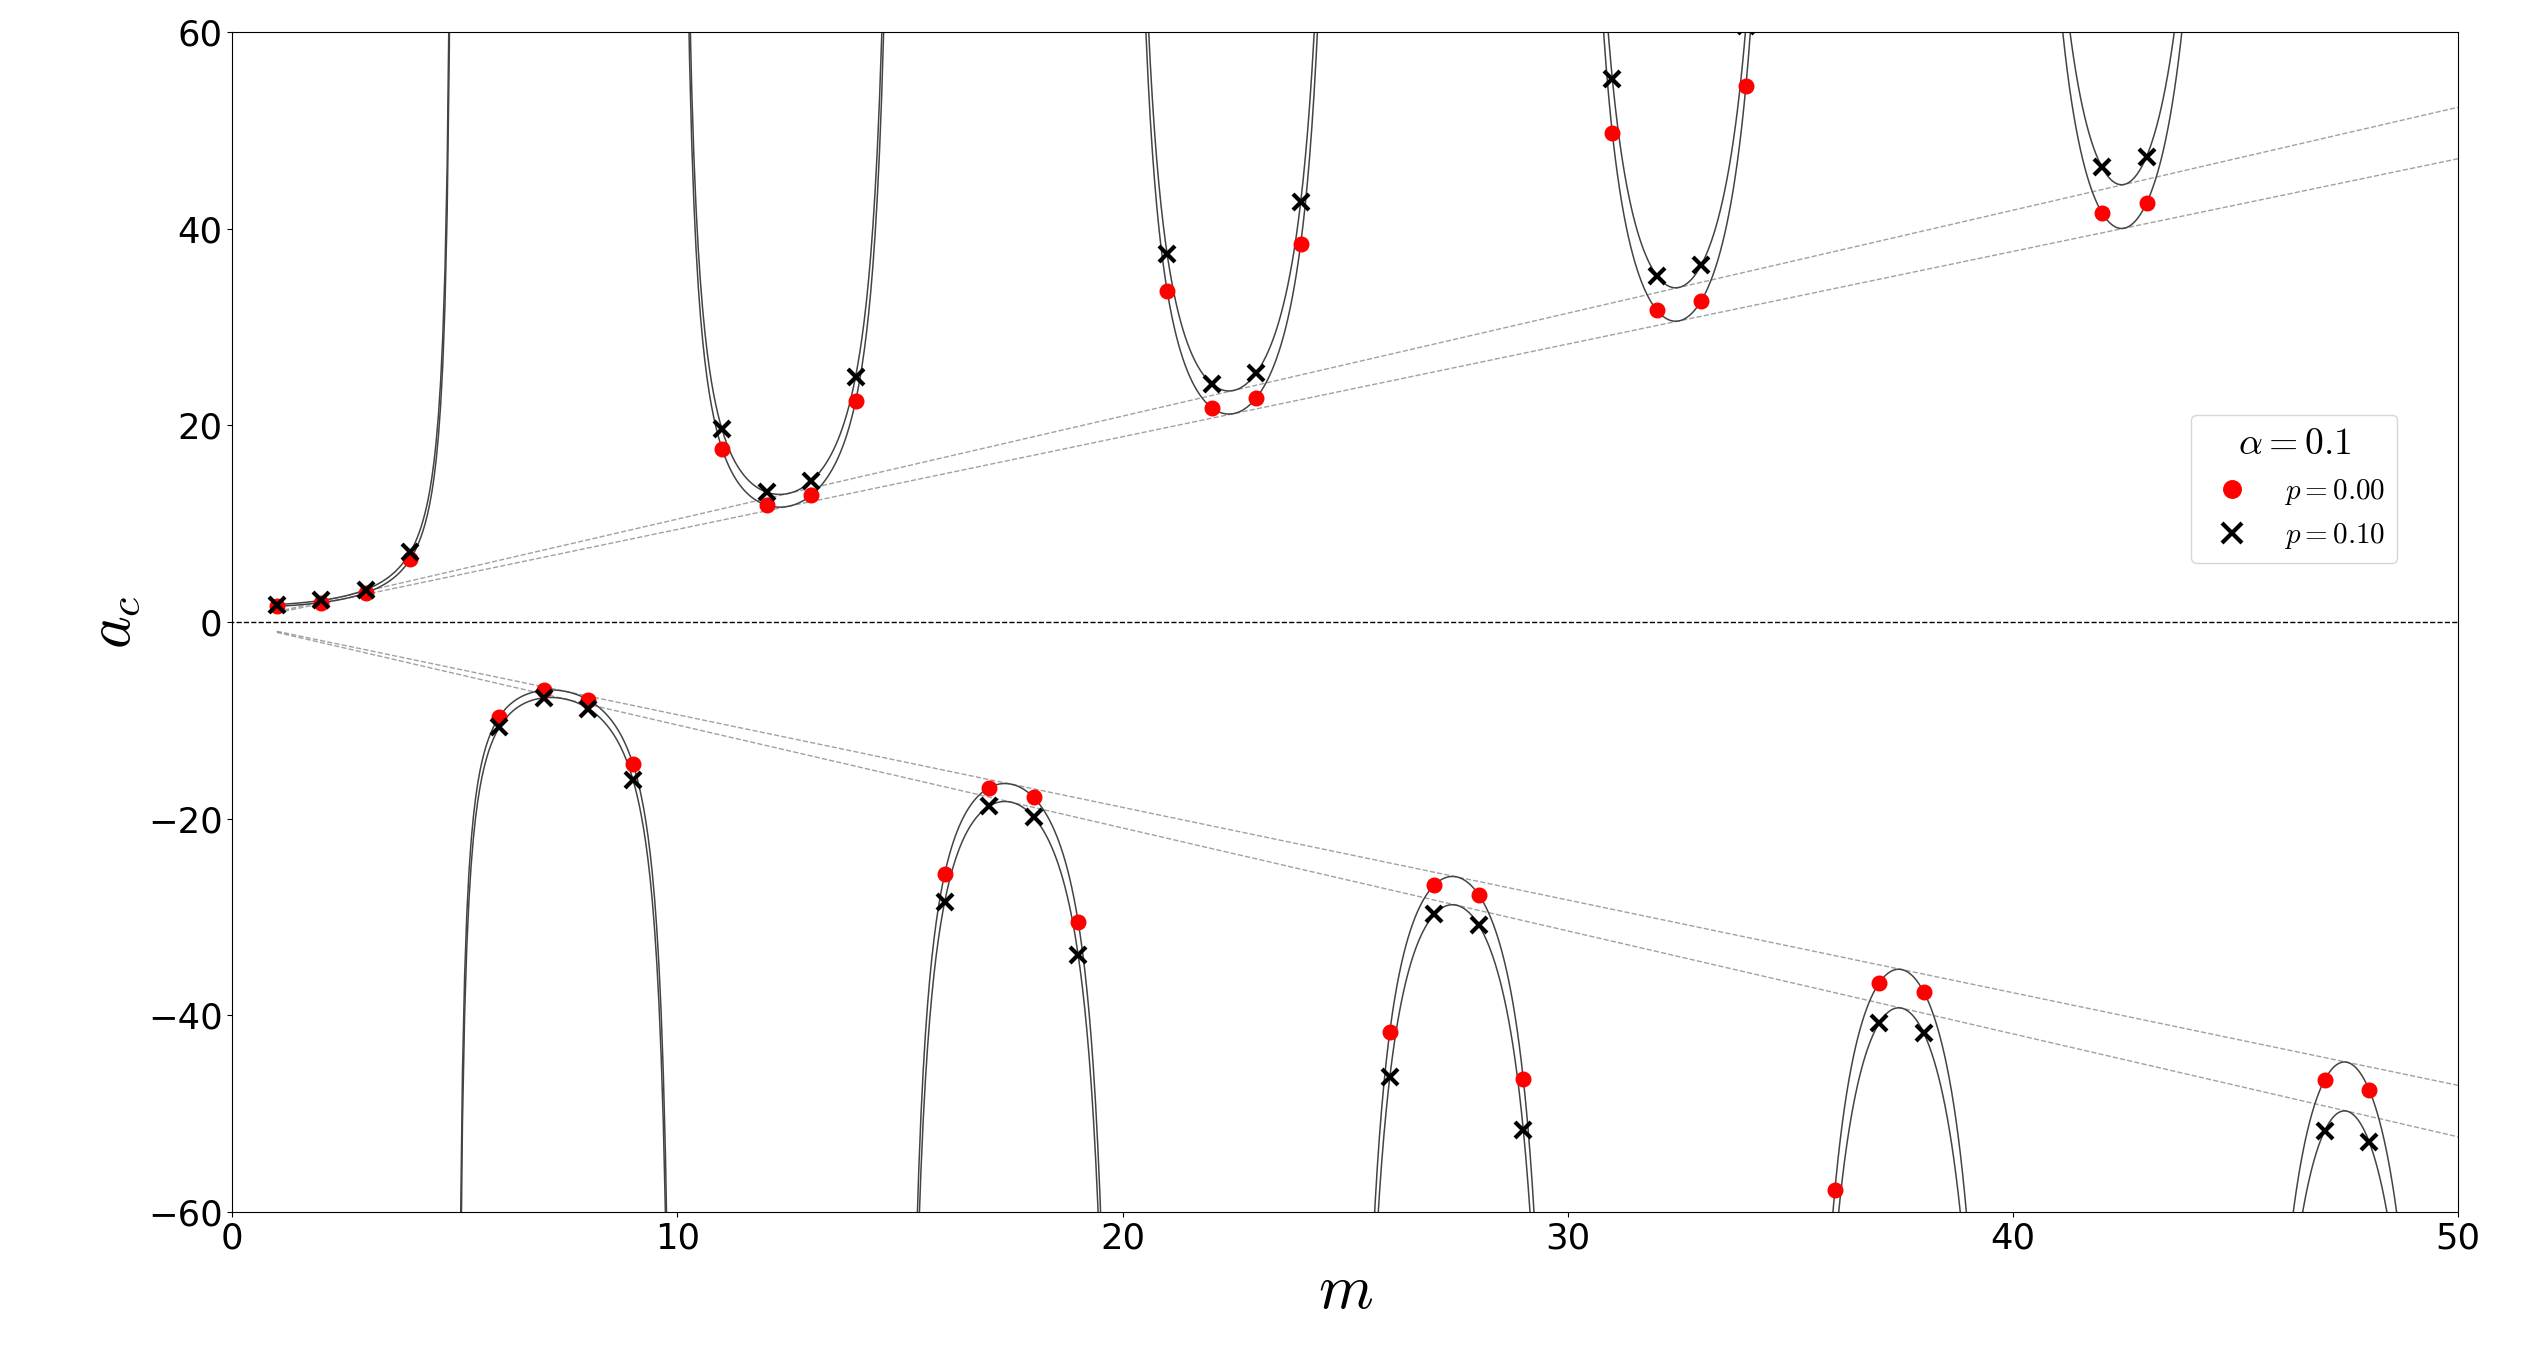
\includegraphics[width=\textwidth]{fig/critical_sequences.png}
  \caption{Critical values for the coupling as the wave number increases for a fixed interaction range of $\alpha=0.1$. The effect of
  increasing $p$ is seen as a steeper slope for both positive and negative critical sequences.}
  \label{fig:criticalsequences}
\end{figure}

\noindent We see that if the coupling strength is decreased (increased) from 0 to more negative (positive) values, wave numbers become
stable one by one. For example, if $\alpha=0.2$ in table~\ref{table:criticalvalues} and we decrease the coupling starting from 0, the
first stable wave number is $m=4$ at the critical value of $a_c=-7.93$. These are the results derived in the work of Escaff et
al.\cite{escaff2014arrays} for the case of $p=0$. In our extension to small-world networks, the effect of increasing $p$ is to make the
critical sequence increase or decrease more sharply, as illustrated in figure~\ref{fig:criticalsequences}. A noteworthy aspect of these
sequences of critical values is that, for negative coupling, the system spontaneously self-organizes to a wave solution when the first
negative critical value is reached. For positive coupling, the first stable solution is the globally synchronized one, with $m=0$ and
critical value of $a_c=1.5$\cite{Wood06a,Wood06b,assis2011infinite,rodrigues2020synchronization}. Therefore, no wave solution will
spontaneously form even when increasing the coupling to arbitrarily large values, since global synchrony is vastly more probable when
starting the system from the quiescent initial state\cite{rodrigues2020synchronization}. For real systems with finite size, we might
expect that fluctuations can induce transitions between different wave numbers for positive values of the coupling parameter, which is
indeed verified in simulations in chapter \ref{chap:simulation}.

\section{Conclusions} In this chapter we have derived a MF approximation for discrete coupled oscillators with natural frequency
distribution $\omega\sim g$ on small-world networks generated by introducing coupling disorder into the regular ring networks. To
obtain analytical results, and derive analogous expressions to previous work, we have restricted these to the regime of small disorder
($p$). It is also implicitly assumed that the behavior of a sufficiently large network will be approximated by the average behavior
over different networks, since the building process for the small-world networks considered here is stochastic. For real finite
systems, it is possible that some realizations of a small-world network will not produce these macroscopic behaviors, since
fluctuations become more dominant as system size is decreased. Nonetheless, the theory predicts some properties that can be tested
through simulation, such as the failure to achieve global synchrony even for large positive couplings depending on initial conditions
and fluctuations, and the change in speed with which these waves travel if there are macroscopic patterns in the spatial distribution
of the natural frequencies of the constituent phase oscillators.

\chapter{Introduction}

Este é o capítulo introdutório com exemplo de uma referência padrão. \textbf{Ressalta-se que o texto: ``Citado na página
...'' é opcional e que outras formatações também podem ser usadas.}
 

\chapter{Comandos básicos do \LaTeX \label{cap1}}


Aqui apresentamos os comandos mais básicos para preparação de um trabalho em \LaTeX. Para mais detalhes sugere-se, por exemplo, ``The
not so short introduction to  \LaTeX\  2$\varepsilon$'', que pode ser obtido em
\url{http://tug.ctan.org/info/lshort/english/lshort.pdf} e o manual da classe \abnTeX\ que foi a classe utilizada
na confecção deste modelo. Perceba que há links no arquivo pdf que permitem clicar sobre o número da referência e ser enviado para
lista de referências e que na última podem ser colocados links para os documentos referenciados.

Comentários em um arquivo \LaTeX\  podem ser introduzidos através do caracter \%. 

\section{Dicas gerais}

A principal dica que daremos neste texto é quanto ao \emph{Character Encoding} a ser usado nos arquivos. A classe \abnTeX, utilizada na
confecção deste modelo, é baseada no \emph{encoding} UTF-8. Desta forma, recomenda-se fortemente que \textbf{todos} os arquivos sigam
este padrão para não haver problemas com acentos, por exemplo. Isto pode ser facilmente configurado na grande maioria dos editores
\LaTeX.

Outra dica importante ao usar o  \LaTeX\ na confecção de trabalhos longos é que se pode dividir o arquivo fonte em vários arquivos e
usar os comandos \verb+\input{arquivo}+ e \verb+\include{arquivo}+. Esta estrutura foi adotada na confecção deste modelo. As diferenças
entre os dois comandos é que no primeiro não são criados os arquivos auxiliares para o arquivo incluído e seu conteúdo não
necessariamente se iniciam em uma nova página, enquanto no segundo arquivos auxiliares próprios são criados e o seu conteúdo se inicia
em uma nova página. A recomendação é que pequenos trechos do trabalho sejam incluídos com o comando \verb+\input+ enquanto trechos
maiores, como um capítulo, por exemplo, sejam incluídos através do comando \verb+\include+. Ao utilizar vários arquivos, apenas o
arquivo fonte principal deve ser compilado. Recomenda-se o uso de editores   \LaTeX\ que permitam a criação de projetos, o que facilita
ainda mais a navegação pelos vários arquivos, a compilação, visualização, etc.  Alguns editores recomendados são: TeXmaker (Linux, Mac,
Windows), TeXstudio (Linux, Mac, Windows), TeXnicCenter (Windows), Kile (Linux). 

\section{Incluindo referências}

Uma das grandes vantagens no uso do \LaTeX\ na confecção de trabalhos acadêmicos é a facilidade de se incluir, numerar e gerenciar
referências bibliográficas através de pacotes como o BibTeX. Desta forma, recomendamos o uso do último para gerenciar suas referências.
A grande maioria dos editores de revistas científicas, assim como o google books e outros sites fornecem arquivos com os dados
bibliográficos em formato BibTeX. Assim, basta criar um arquivo, com extensão \verb+.bib+, que contenha os dados das referências usadas
e adicioná-lo ao arquivo fonte, em local apropriado, através do comando \verb+\bibliography{nome_do_arquivo.bib}+. É importante
salientar que o uso correto do BibTeX depende de uma compilação inicial do arquivo fonte \LaTeX, seguida da compilação BibTeX e mais
duas compilações   \LaTeX. Isto permite a criação da lista de referências e o correto ordenamento destas ao longo do texto e na seção
de referências. De fato, o arquivo \verb+.bib+ pode conter muito mais referências que as efetivamente utilizadas no texto de forma que
apenas as que forem citadas no texto serão incluídas na seção de referências.  Além disso, a formatação que será dada à lista de
referências, assim como as informações disponíveis no arquivo \verb+.bib+ que serão efetivamente utilizadas, são definidas pelo padrão
adotado para as referências. Sugere-se que o formato a ser adotado seja o formato \verb+unsrt+ que foi selecionado neste documento
através dos comandos:\\ \verb+\usepackage[fixlanguage]{babelbib}+\\ \verb+\selectbiblanguage{brazil}+\\
\verb+\bibliographystyle{babunsrt}+\\ em locais apropriados. Além disso, alguns dos editores recomendados anteriormente permitem o
gerenciamento inclusive das referências ao se criar um projeto, o que facilita enormemente a inclusão de novas citações no texto.

Cada entrada do arquivo \verb+.bib+ tem estrutura similar à mostrada abaixo:
\begin{verbatim}
    @article{exemplo,
    author={ R. M. Herman and A. Asgharian},
    journal={J. Mol. Spectrosc.},
    volume={19},
    pages={305},
    year={1966},
    }
\end{verbatim}

Para fazer uma citação à esta referência basta incluir o comando \verb+\cite{exemplo}+, o que produz:. A formatação dada
a cada entrada depende do estilo selecionado. Para exemplificar, seguem citações a vários documentos que foram retiradas dos modelos do
\abnTeX\:.
\textbf{Ressalta-se que o texto: ``Citado na página ...'' presente na lista de referências é opcional e que outras formatações podem
ser usadas.}

\newpage


\section{\label{estruturacao}Estruturação do texto}

Para iniciar este capítulo utilizamos o comando \\ \verb+\chapter{Comandos básicos do \LaTeX \label{cap1}}+.\\ O comando
\verb+\label{cap1}+ é opcional e foi introduzido para permitir posteriores referências ao capítulo. Por exemplo, o comando
\verb+\ref{cap1}+, produz o seguinte resultado: \ref{cap1}, e pode ser usado para fazer referências a este capítulo ao longo do texto.
A numeração é automaticamente atualizada caso um novo capítulo seja introduzido. De fato, qualquer parte do texto, figuras, tabelas,
equações, etc podem ser nomeadas pelo comando \verb+\label+ e posteriormente referenciadas pelo comando \verb+\ref+.

Seções dentro de um capítulo podem ser introduzidas pelo comando \\ \verb+\section{\label{estruturacao}Estruturação do texto}+. \\
Subseções são incluídas com o comando \verb+\subsection{Nome da subseção}+. Pode-se também usar \verb+\subsubsection+ e assim por
diante. Caso o capítulo ou seção tenham um nome muito grande pode-se optar por introduzir um  nome resumido para o sumário e cabeçalho
das páginas usando, por exemplo, \verb+\section[título resumido]{título longo}+.

\section{Equações, figuras e tabelas}

\subsection{Equações}

Equações podem ser inseridas através do ambiente \verb+equation+. Como exemplo, o comando:
\begin{verbatim}
\begin{equation}
\label{Z1}
Z=\sum_E g(E) e^{-\beta E}=e^{-\beta \epsilon_0}\sum_n g_n \left 
( e^{-\beta \epsilon}\right )^n=e^{-\beta \epsilon_0}\sum_n g_n z^n,
\end{equation}
\end{verbatim}
produz a seguinte equação:
\begin{equation}
\label{Z1}
Z=\sum_E g(E) e^{-\beta E}=e^{-\beta \epsilon_0}\sum_n g_n \left 
( e^{-\beta \epsilon}\right )^n=e^{-\beta \epsilon_0}\sum_n g_n z^n,
\end{equation}
Podemos, então, no texto introduzir facilmente referências à equação \ref{Z1} usando o comando \verb+\ref{Z1}+.

\subsection{Figuras}

Figuras podem ser introduzidas usando o comando, retirado da Ref.~:
\begin{verbatim}
\begin{figure}[htb]
	\caption{\label{fig_grafico}Gráfico produzido em Excel e salvo como PDF}
	\begin{center}
	    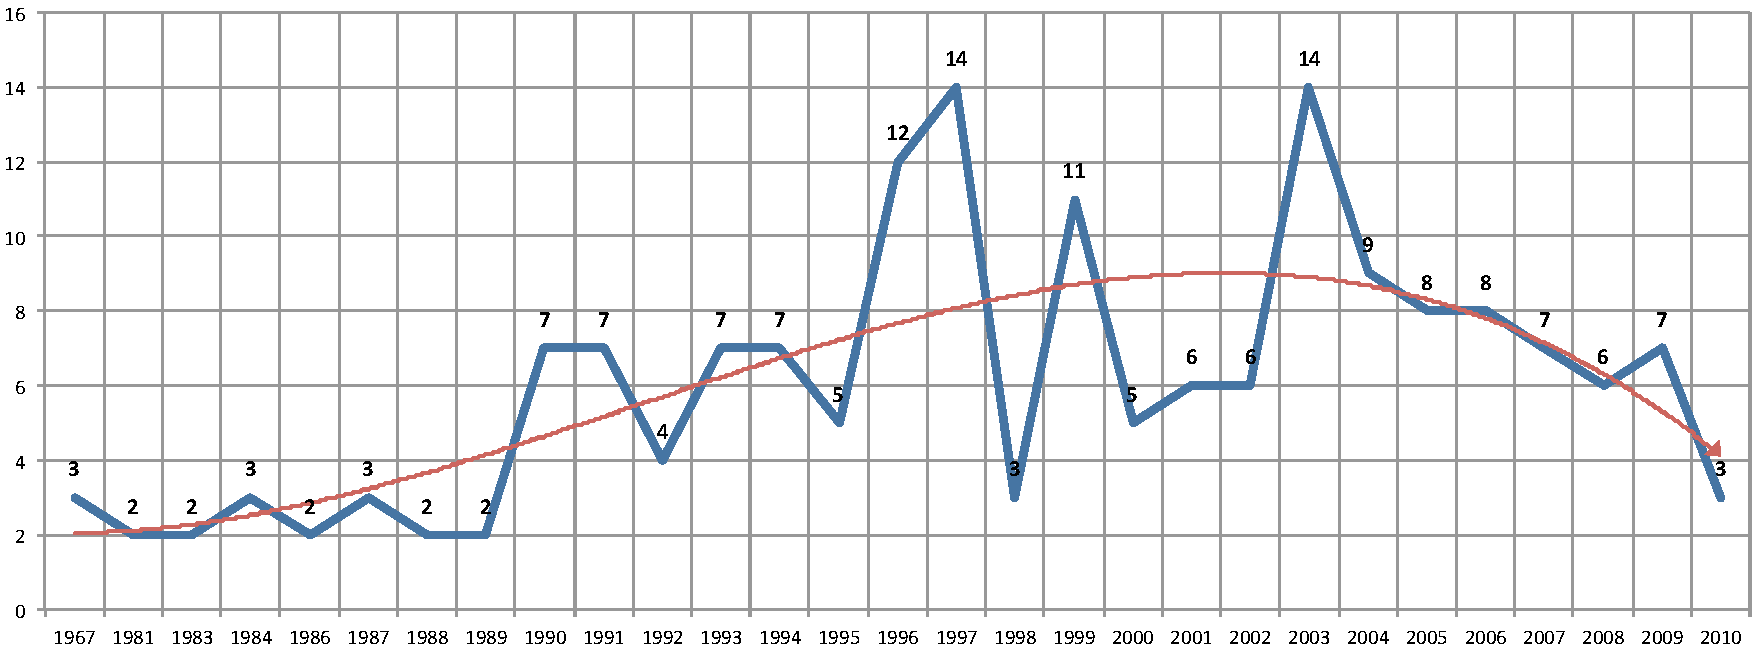
\includegraphics[scale=0.5]{fig/abntex2-modelo-img-grafico.pdf}
	\end{center}
	\legend{Fonte: \cite[p. 24]{araujo2012}}
\end{figure}
\end{verbatim}

Ressalta-se que ao invés de estabelecer a escala da figura através do comando \verb+scale=0.5+, poderia-se definir sua largura ou
altura através de \verb+width+ ou \verb+height+ usando, por exemplo, \\
\verb+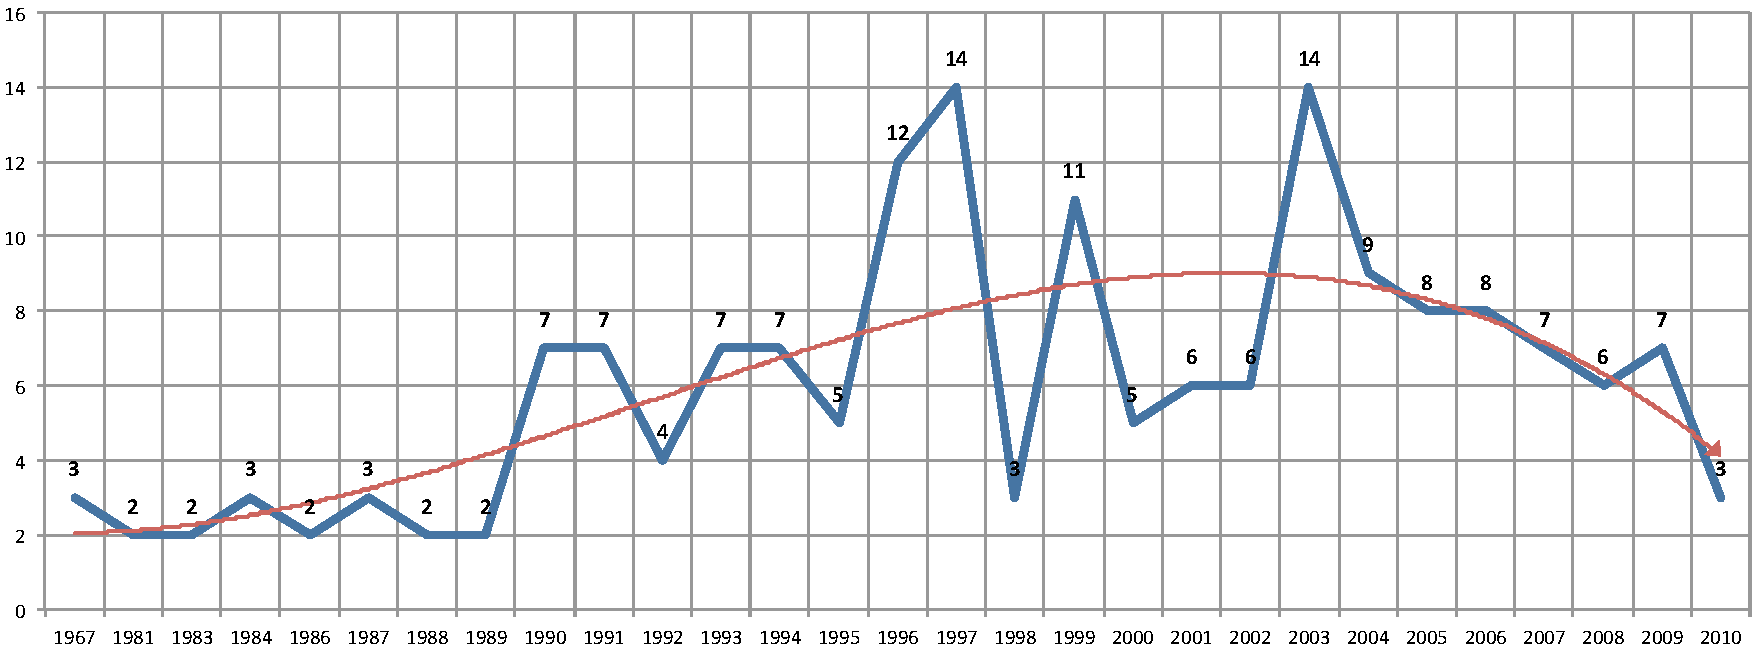
\includegraphics[width=5cm]{fig/abntex2-modelo-img-grafico.pdf}+ que re-escalaria a figura de forma a ela ficar com 5 cm de
largura. Pode-se ainda usar \verb+0.5\linewidth+ ao invés de \verb+5cm+ para estabelecer a largura da figura como sendo metade da
largura da linha do texto. O posicionamento da figura é definido pelo próprio \LaTeX. Recomenda-se colocar o comando o mais próximo
possível do lugar onde a figura é citada. Por fim, recomenda-se usar figuras em formato \verb+pdf+.

\begin{figure}[htb]
	\caption{\label{fig_grafico}Gráfico produzido em Excel e salvo como PDF}
	\begin{center}
	    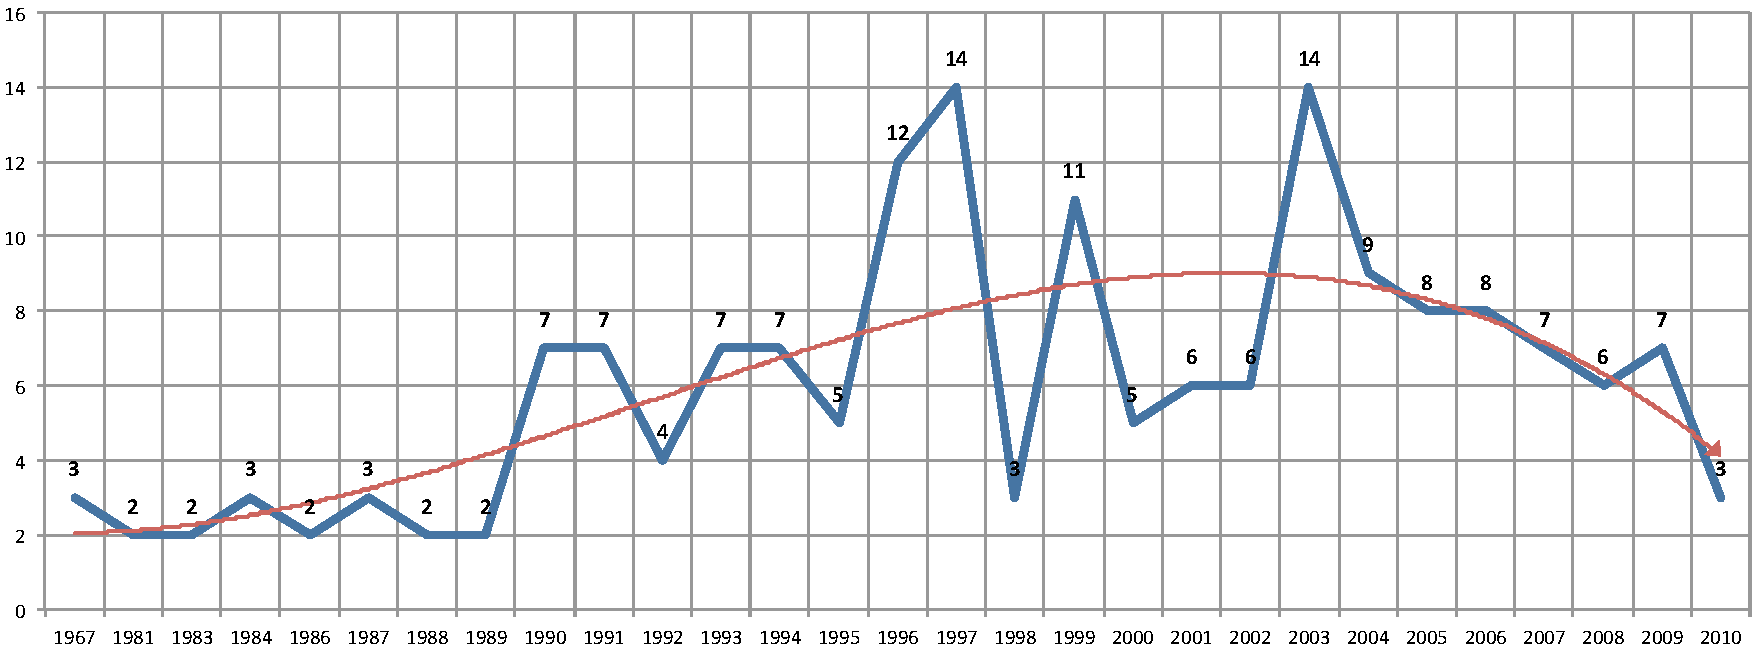
\includegraphics[scale=0.5]{fig/abntex2-modelo-img-grafico.pdf}
	\end{center}
	\legend{Fonte:}
\end{figure}


\subsection{Tabelas}

Há de se admitir que a confecção de tabelas em \LaTeX\ envolve uma prática um pouco maior. Abaixo apresentamos o comando que gerou a
Tabela~\ref{tab1}. Uma dica interessante é que o comando \verb+\resizebox+ permite ajustar a tabela à largura do texto e é
especialmente útil em situações onde a largura da tabela seria maior que a largura do texto.
\begin{scriptsize}
\begin{verbatim}
\begin{table}[ht] 
    \caption{Publicações relacionadas a alguma área em periódicos selecionados.
    \label{tab1}}
		\resizebox{\linewidth}{!}{%
\begin{tabular}{|l|c|c|c|c|c|c|c|c|c|}
    \hline
\multirow{2}{*}{\textbf{PERIÓDICO}} & \multicolumn{9}{c|}{ANOS}
\\ \cline{2-10}
& 2009&	2010&	2011&	2012&	2013&	2014&	2015& 2016& 2017\\ \hline
\textit{International Journal of Something} &	13&	15&	16&	15&	17&	17&	22& 22& 14\\ \hline 
\textit{Text Horizons}               		& 	6&	6&	9&	6&	8&	7&	19& 7& 6\\ \hline 
\textit{The Blablabla Review}             & 	8&	14&	9&	9&	15&	13&	21& 15& 9\\ \hline 
\textit{Journal of Magic}		&	2&	4&	2&	5&	1&	5&	1& 7& 4\\ \hline 
\textbf{TOTAL}&                           	29&	39&	36&	35&	41&	42&	63& 51& 33\\ \hline 
\multicolumn{8}{l}{Confeccionado pelo autor.}
\end{tabular}%
}
\end{table}
\end{verbatim}
\end{scriptsize}

\begin{table}[ht] 
    \caption{Publicações relacionadas a alguma área em periódicos selecionados.
    \label{tab1}}
		\resizebox{\linewidth}{!}{%
\begin{tabular}{|l|c|c|c|c|c|c|c|c|c|}
    \hline
\multirow{2}{*}{\textbf{PERIÓDICO}} & \multicolumn{9}{c|}{ANOS}
\\ \cline{2-10}
& 2009&	2010&	2011&	2012&	2013&	2014&	2015& 2016& 2017\\ \hline
\textit{International Journal of Something} &	13&	15&	16&	15&	17&	17&	22& 22& 14\\ \hline 
\textit{Text Horizons}               		& 	6&	6&	9&	6&	8&	7&	19& 7& 6\\ \hline 
\textit{The Blablabla Review}             & 	8&	14&	9&	9&	15&	13&	21& 15& 9\\ \hline 
\textit{Journal of Magic}		&	2&	4&	2&	5&	1&	5&	1& 7& 4\\ \hline 
\textbf{TOTAL}&                           	29&	39&	36&	35&	41&	42&	63& 51& 33\\ \hline 
\multicolumn{8}{l}{Confeccionado pelo autor.}
\end{tabular}%
}
\end{table}


\chapter{Conclusions}

Conclusões.




% ----------------------------------------------------------
% ELEMENTOS PÓS-TEXTUAIS
% ----------------------------------------------------------
\postextual
% ----------------------------------------------------------

% ----------------------------------------------------------
% Referências bibliográficas
% ----------------------------------------------------------
\bibliographystyle{babunsrt}
\bibliography{tex/references.bib}

% ----------------------------------------------------------
% Glossário
% ----------------------------------------------------------
%
% Consulte o manual da classe abntex2 para orientações sobre o glossário.
%
%\glossary

% ----------------------------------------------------------
% Apêndices
% ----------------------------------------------------------

% ---
% Inicia os apêndices
% ---
\begin{apendicesenv}

% Imprime uma página indicando o início dos apêndices
\partapendices

% ----------------------------------------------------------
\chapter{\label{appendix:LC}Path length and clustering for regular ring lattices}
% ----------------------------------------------------------

\section{Average Path Length}

The distance $L_{ij}$ between two nodes $i$ and $j$ is the minimum number of edges that must be traversed to connect them. The average
path length is defined as the average distance between every possible pair of nodes in the network. For a network with $N$ nodes this
is:

\begin{equation}
    L = \frac{2}{N^2-N}\sum_{i<j}L_{ij}
\end{equation}

Consider the lowest node in a ring graph with $N$ nodes and $2K$ neighbors per node. Going counterclockwise (CCW), there are $K$ nodes
at distance $1$, then $K$ nodes at distance $2$ and so on until we reach some region near the top. In total, there will be $G$ groups
of nodes, each with $K$ nodes, at distances $1,2,3...,G$ from our starting point at the bottom. $G$ is given by the largest integer
smaller than $(N-1)/(2K)$. This can be written with the floor operation:

\begin{equation}
    G=\floor*{\frac{N-1}{2K}}
\end{equation}

This same procedure can be performed from the clockwise (CW) direction. Thus, there are $2K$ nodes at distance $1$ and so on up to
distance $G$. The last group of nodes at the top is therefore at a distance $G+1$, but it contains less than $2K$ nodes. Indeed, it
contains a number $R$ of nodes equal to the remainder of the integer division of $N-1$ by $2K$:

\begin{equation}
    R = N - 1 - 2KG
    \label{eq:R}
\end{equation}

\noindent This reasoning can be visualized in Fig.~\ref{fig:Lgroups}.

\begin{figure}
\centering
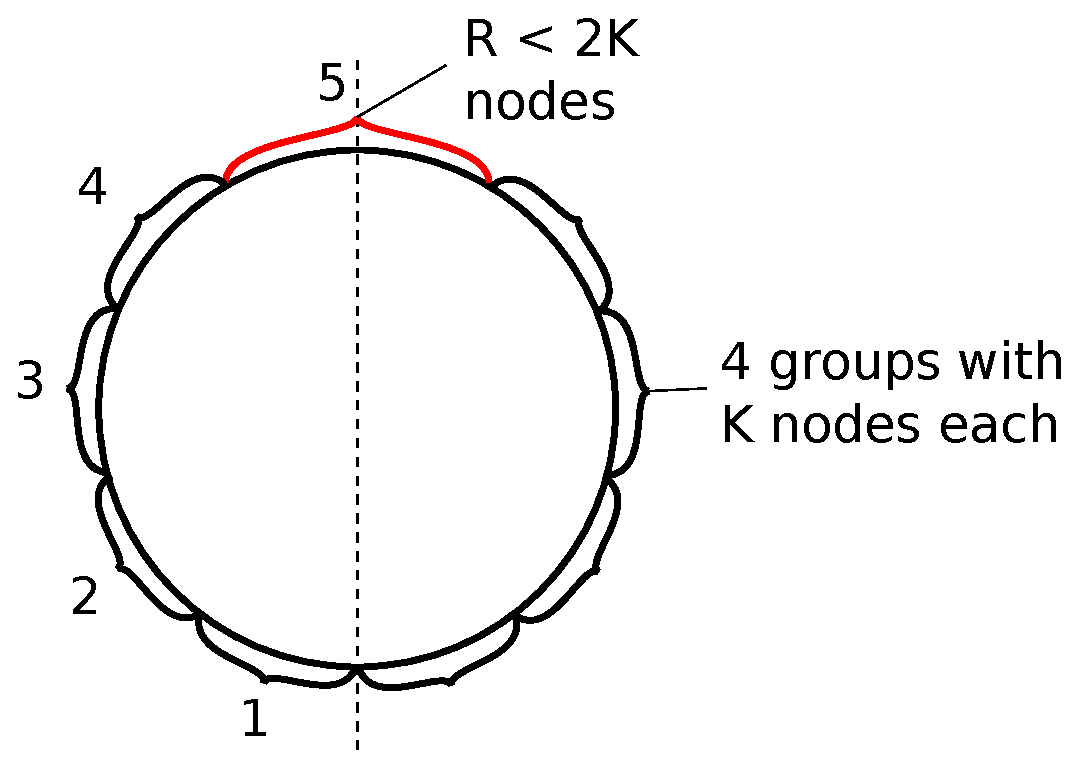
\includegraphics[width=0.6\textwidth]{fig/path_length_groups.eps}
\caption{Counting the number of nodes at distances visually. Here $G=4$ groups at distances $1,2,3,4$ from the bottom node.}
\label{fig:Lgroups}
\end{figure}

Since there are $N-1$ pairs between the bottom node and all other nodes in the lattice, the average distance $L_0$ between the bottom
node and all other nodes is then given by:

\begin{align}
    L_0 &= \frac{1}{N-1} \left[ 2K \sum_{i=1}^Gi + R(G+1) \right] \notag \\[9pt]
        &= \frac{1}{N-1} \left[ KG(G+1) + R(G+1) \right] \notag \\[9pt]
    L_0 &= \left(G + 1\right) \left( 1 - \frac{KG}{N-1} \right)
\end{align}

\noindent where we used equation \ref{eq:R} to substitute in for $R$.  Because we started with an arbitrary node at the bottom, this
result is true for any given node in a regular ring, and thus we conclude that the average path length for the whole network is just
$L_0$.

\begin{align}
    L(N,K) = \left(G + 1\right) \left( 1 - \frac{KG}{N-1} \right) \notag \\[9pt]
    \text{with} \qquad G=\floor*{\frac{N-1}{2K}}
\end{align}

\section{Average Clustering}

The clustering coefficient for a node $i$ in the graph is defined as: let $n_i$ be the number of neighbors of some node $i$. Then,
there are at most $(n_i^2-n_i)/2$ connections between any two of its neighbors. Let $m_i$ be the number of actual connections that are
present in a particular graph. Then, the clustering coefficient $C_i$ of node $i$ is given by:

\begin{equation}
    C_i = \frac{2m_i}{n_i^2-n_i}
\end{equation}

\noindent If there are $N$ nodes in the graph, the average clustering
coefficient is thus given by:

\begin{equation}
    C = \frac{1}{N}\sum^N_{i=1} C_i
\end{equation}

First, consider a ``close-up" of a section of a regular ring where $N\gg K$.  Consider a node $i$ with $K$ CW neighbors and $K$ CCW
neighbors. Let $m$ be the number of connections between neighbors of node $i$. We can manually count $m$ for some values of $K$:

\begin{figure}
\centering
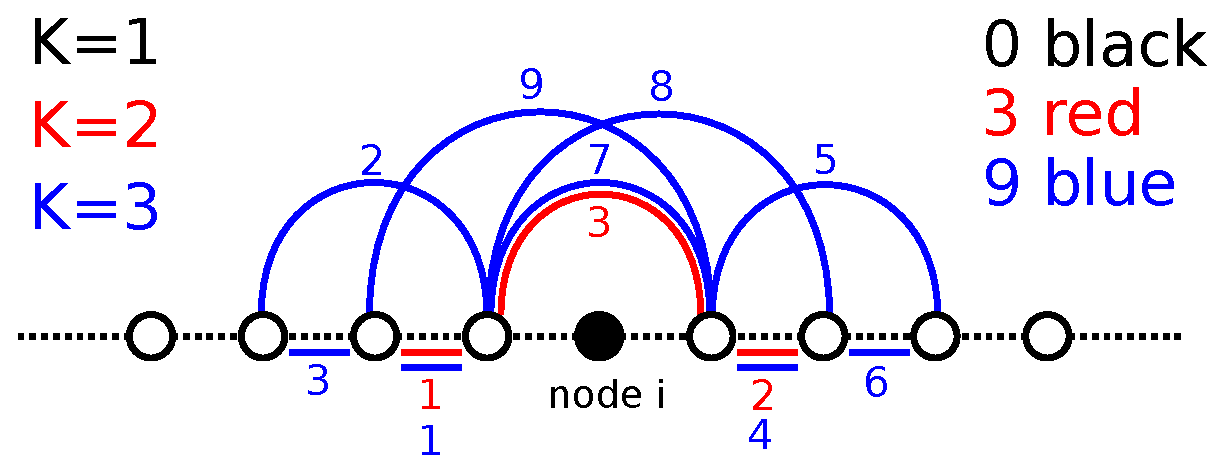
\includegraphics[width=0.75\textwidth]{fig/clustering.eps}
\caption{ (Color online) Counting $m$ for $k=1,2,3$. We note three contributions to $m$: a fully connected group of $K$ CW neighbors
(left), a fully connected group of $K$ CCW neighbors (right) and connections that go ``over" the center node.  }
\label{fig:clustering}
\end{figure}

\begin{align*}
    m &= 0 \qquad \text{if} \qquad K \leq 1\\
    m &= 3 \qquad \text{if} \qquad K = 2\\
    m &= 9 \qquad \text{if} \qquad K = 3
\end{align*}

The general case for $N \gg K$ can be counted by summing the contributions of the three groups as shown in figure \ref{fig:clustering}.
Two fully connected groups of $K$ nodes each contributes with $(K^2-K)$ connections. The connections that bypass node $i$ also
contribute with $(K^2-K)/2$ connections and thus we have.

\begin{align}
    m &= \frac{3}{2}(K^2-K)
    \label{eq:m}
\end{align}

\noindent Now we divide equation \ref{eq:m} by the total number of connections between the $2K$ neighbors of node $i$ to get its
clustering coefficient $C_i$:

\begin{align}
    C_i(N,K) = \frac{3K-3}{4K-2}
    \label{eq:ci}
\end{align}


\begin{figure}
\centering
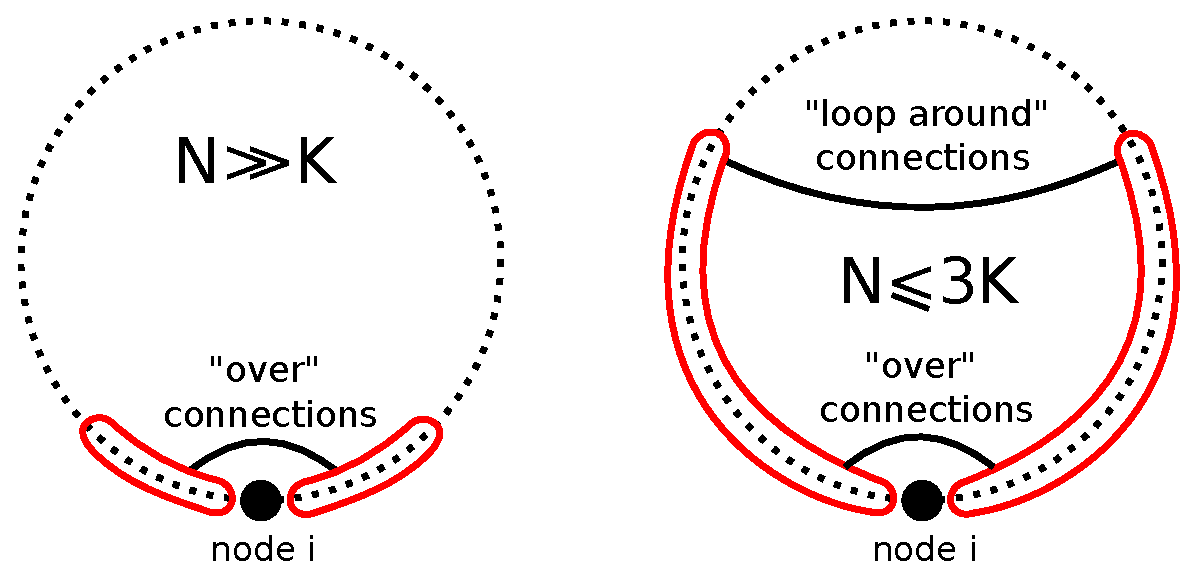
\includegraphics[width=0.9\textwidth]{fig/clustering-loop.eps}
\caption{ Connections that contribute to the clustering coefficient of node $i$.  The red regions represent the CW and CCW groups of
neighbors of node $i$, and they are fully connected each within itself. Additional connections are made going ``over" node $i$, but
when $N\leq3K$ there are additional connections that loop around the opposite side of the lattice.  }
\label{fig:loop}
\end{figure}

\noindent When $N$ is not so large compared to $K$, additional connections between the CCW and CW neighbors may appear by looping
around the opposite side of node $i$, as depicted in figure \ref{fig:loop}. These additional connections will be present whenever the
remaining nodes that are neither in the CW or CCW group are fewer than $K$. The number of such nodes is just $N-2K-1$, which gives us
the condition $N\leq 3K$ for additional connections to be present.


The number of ``loop around" connections that will be present will depend on how many nodes there are in the remaining group after
removing node $i$ and its immediate neighbors. Let this number be denoted by $D=N-2K-1$. Then, the number of additional connections
will be given by

\begin{align}
    (K-D) + (K-D-1) + ... + 2 + 1 = \frac{(K-D+1)(K-D)}{2}
    \label{eq:looparound}
\end{align}

Adding equation \ref{eq:looparound} to \ref{eq:m} we get

\begin{align}
    m = \frac{3}{2}(K^2 - K) + \frac{1}{2}(3K-N+1)(3K-N+2)
\end{align}

And thus the clustering now becomes:

\begin{align}
    C_i(N,K) = \frac{3K-3}{4K-2} + \frac{(3K-N+1)(3K-N+2)}{4K^2-2K}
    \label{eq:ci1}
\end{align}

This formula holds up to the point when $D=0$ or $N=2K+1$. For all values $D\leq 0$ the regular ring is in fact a complete graph, where
every node connects to every other. In these cases the clustering coefficient is always equal to one.  Formulas \ref{eq:ci} and
\ref{eq:ci1} together offer a complete expression for the clustering of node $i$. Since $C_i=C_j \quad \forall i,j$, this is just the
average clustering of the whole network and we finally get:

\begin{align}
    C(N,K) =
    \begin{cases}
        \frac{3K-3}{4K-2} \quad &\text{if} \quad N>3K \\[9pt]
        \frac{3K-3}{4K-2} + \frac{(3K-N+1)(3K-N+2)}{4K^2-2K} \quad &\text{if}
        \quad 3K \geq N > 2K+1 \\[9pt]
        1 \quad &\text{else}
    \end{cases}
    \label{eq:ci2}
\end{align}


\end{apendicesenv}


% ----------------------------------------------------------
% Annex
% ----------------------------------------------------------
%\begin{anexosenv}
%
%
%\partanexos  % Print annex front page
%
%\chapter{My annex 1}
%\chapter{My annex 2}
%
%
%\end{anexosenv}

%---------------------------------------------------------------------
% INDICE REMISSIVO - ELEMENTO OPCIONAL
%---------------------------------------------------------------------
%\phantompart
%\printindex
%---------------------------------------------------------------------


\end{document}
